\documentclass[a4paper,11pt]{article}
\usepackage[table]{xcolor}



\newcommand{\defeq}{\mathrel{\doteq}}

\newcommand{\lzero}{0}

\newcommand{\kw}[1]{\mathtt{#1}}

\newcommand{\expr}{e}
\newcommand{\vall}{w}
\newcommand{\valr}{v}
\newcommand{\eif}{\kw{if}}
\newcommand{\eapp}{\;}
\newcommand{\eprojl}{\kw{fst}}
\newcommand{\eprojr}{\kw{snd}}
%\newcommand{\eprov}[1]{\eta_{#1}}
\newcommand{\etrue}{\kw{true}}
\newcommand{\efalse}{\kw{false}}
\newcommand{\econst}{c}
\newcommand{\eop}{\delta}
\newcommand{\efix}{\mathop{\kw{fix}}}
%\newcommand{\labelA}{\ell}

\newcommand{\tr}{T}
\newcommand{\trift}{\eif^{\kw{t}}}
\newcommand{\triff}{\eif^{\kw{f}}}
\newcommand{\trprojl}{\eprojl}
\newcommand{\trprojr}{\eprojr}
\newcommand{\trtrue}{\etrue}
\newcommand{\trfalse}{\efalse}
\newcommand{\trconst}{\econst}
\newcommand{\trop}{\eop}
\newcommand{\trfix}{\efix}
\newcommand{\trapp}[5]{#1 \; #2 \mathrel{\triangleright} {\efix #3(#4).#5}}

\newcommand{\adap}{\kw{adap}}
\newcommand{\ddep}[1]{\kw{depth}_{#1}}
\newcommand{\nat}{\mathbb{N}}
\newcommand{\natb}{\nat_{\bot}}
\newcommand{\natbi}{\natb^\infty}
\newcommand{\nnatA}{n}
\newcommand{\nnatB}{m}
\newcommand{\nnatbA}{s}
\newcommand{\nnatbB}{t}
\newcommand{\nnatbiA}{q}
\newcommand{\nnatbiB}{r}

\newcommand{\type}{\tau}
\newcommand{\tbase}{\kw{b}}
\newcommand{\tbool}{\kw{bool}}
\newcommand{\tarr}[5]{#1; #3 \xrightarrow{#4; \, #5} #2}
\newcommand{\env}{\theta}

\newcommand{\bigstep}{\mathrel{\Downarrow}}

\newcommand{\dmap}{\rho}
\newcommand{\dmapb}{\bot_\dmap}
\newcommand{\supp}{\kw{supp}}
\newcommand{\dom}{\kw{dom}}

\newcommand{\tvdash}[1]{\vdash_{#1}}

%Packages
\usepackage[T1]{fontenc}
\usepackage{fourier} 
\usepackage[english]{babel} 
\usepackage{amsmath,amsfonts} 
\usepackage{amsthm} 
\usepackage{color}   %May be necessary if you want to color links
\usepackage{hyperref}
\usepackage{lscape}
\usepackage{geometry}
\usepackage{amsmath}
\usepackage{algorithm}
\usepackage{algorithmic}
\usepackage{amssymb}
\usepackage{amsfonts}
\usepackage{times}
\usepackage{bm}
\usepackage{ stmaryrd }
\SetSymbolFont{stmry}{bold}{U}{stmry}{m}{n}

\usepackage{ amssymb }
\usepackage{ textcomp }
\usepackage[normalem]{ulem}
% For derivation rules
\usepackage{mathpartir}
\usepackage{color}
\usepackage{a4wide}
\usepackage{caption}
\usepackage{subcaption}
\usepackage{mathpartir}
\usepackage{amsmath,amsfonts}
\usepackage{ amssymb }
\usepackage{color}
\usepackage{algorithm}
\usepackage{algorithmic}
\usepackage{microtype}
\usepackage{eucal}
\usepackage{url}
\usepackage{xspace}
\usepackage{array}
\usepackage{listings}

\usepackage{tikz}
\usetikzlibrary{shapes.geometric}
\usetikzlibrary{arrows.meta,arrows}
\usetikzlibrary{decorations.text}
% % % % 


\usepackage{multirow}


%%%%%%%%%%%%%%%%%%%%%%%%%%%%%%%%%%%%%%%%%%%%%%%%%%%%%Packages And Definitions For Listing the Code%%%%%%%%%%%%%%%%%%%%%%%%%%%%%%%%%%%%%%%%%%%%%%%%%%%%%%%%%%%%%%%%%%%%%%%%
\usepackage{listings}
\usepackage{xcolor}

\definecolor{codegreen}{rgb}{0,0.6,0}
\definecolor{codegray}{rgb}{0.5,0.5,0.5}
\definecolor{codepurple}{rgb}{0.58,0,0.82}
\definecolor{backcolour}{rgb}{0.95,0.95,0.92}

\lstdefinestyle{mystyle}{
    backgroundcolor=\color{backcolour},   
    commentstyle=\color{codegreen},
    keywordstyle=\color{magenta},
    numberstyle=\tiny\color{codegray},
    stringstyle=\color{codepurple},
    basicstyle=\ttfamily\footnotesize,
    breakatwhitespace=false,         
    breaklines=true,                 
    captionpos=b,                    
    keepspaces=true,                 
    numbers=left,                    
    numbersep=5pt,                  
    showspaces=false,                
    showstringspaces=false,
    showtabs=false,                  
    tabsize=2
}

\lstset{style=mystyle}

\usepackage{tikz}
\usetikzlibrary{shapes,arrows}
\newcommand{\THESYSTEM}{\textsf{AdaptFun}}

% Define block styles
\tikzstyle{decision} = [diamond, draw, fill=blue!20, 
    text width=4.5em, text badly centered, node distance=3cm, inner sep=0pt]
\tikzstyle{block} = [rectangle, draw, fill=blue!20, 
    text width=5em, text centered, rounded corners, minimum height=4em]
\tikzstyle{line} = [draw, -latex']
\tikzstyle{cloud} = [draw, ellipse,fill=red!20, node distance=3cm,
    minimum height=2em]

\begin{document}
\title{Appendix for "Program analysis for Adaptivity Analysis"}

\author{}

\date{}

\maketitle

In this appendix, we present three languages: high level loop language, low level loop language, SSA language. In the paper, we choose to only use high level loop language and SSA language. The use of low level language helps us to divide control dependency and data dependency, which is useful in designing the framework. So we keep the low level language in the appendix. 
% \begin{abstract}
%   A data analysis is said to \emph{generalize} when it allows one to draw
%   conclusions from the data that are true of the population from which
%   the data are sampled. Statistician and data scientist have devised
%   several methods aimed to guarantee generalization in  data
%   analyses, and avoid in this way overfitting to the
%   data. Guaranteeing generalization is more difficult when data
%   analyses are \emph{adaptive}: when the result of an analysis depends
%   on the result of previous analyses. 

%   A recent line of work focuses on methods aimed at guaranteeing
%   generalization in adaptive data analysis through the addition of
%   carefully calibrated statistical noise to the empirical results of
%   the analysis on the sampled data. In these works, the confidence
%   intervals on the generalization error that one can achieve for a
%   given analysis usually depend on the \emph{level of adaptivity} of
%   the analysis: the number of adaptive steps that depend on
%   each other. 

%   In this work we introduce a programming framework, named \THESYSTEM,  aimed at
%   supporting the study of the generalization error for adaptive data
%   analysis. Through its analysis system, an upper bound on the
%   adaptivity -- depth (the length of the longest chain of queries) of
%   a program implementing an adaptive data analysis can be overestimated. We show how this language can help to analyze the generalization error between two data analyses with different adaptivity structures.
% \end{abstract}

\tableofcontents


% \section{Introduction}
\section{System Overview}


In adaptive data analysis, a data analysis can depend on the results of
previous analysis over the same data. This dependency may affect the
\emph{generalization properties of the data analysis}. To study this phenomenon
in a formal way, we consider the \emph{statistical query
  model}. In this model, a dataset $X$ consisting of $d$ attributes (columns) and $n$
individuals' data (rows) can be accessed only through an interface to
which one can submit statistical queries. More precisely, suppose that
the type of a row is $R$ (as an example, a row with $d$ binary
attributes would have type $R=\{0,1\}^d$. Then, in the statistical
query model one can access the dataset only by submitting a query to
the interface, in
the form of a function
$p:D\to [0,1] $ where $D$ represents dataset. The collected answer of
the asked query is the average result of $p$ on each row in the
dataset $D$. For example, the result is the
value $\frac{1}{n}\sum_{i=1}^n p(X_i)$ where
$X_i$ is the row of index $i$ in $X$. While this model is rather
simple, in fact it supports sufficient statistics one may be
interested.
% \begin{figure}
%     \centering    \begin{tikzpicture}{node distance = 2cm, auto}
%   % nodes
%   \node [block](high){High level Program P } ;
%   \node [block, right of = high, node distance = 5cm](low){Low level Program $P^*$  } ;
%   \node [block, right of = low, node distance = 8cm](ssa) {SSA form};
%   \node [block, below of = ssa, node distance = 3cm] (bound) { Upper bound} ;
%   \node [block, below of = low, node distance = 3cm](adaptlow){Low level adaptivity $A^*$};
%   \node [block, below of = high, node distance = 3cm](adapthigh){High level adaptivity $A$};
%   % edges
%   \path [line] (high) -- node {translate} (low) ;
%   \path [line] (low) -- node {transformation} (ssa);
%   \path [line] (ssa) -- node {\THESYSTEM} (bound);
%   \path [line] (bound) --  (adaptlow);
%   \path [line] (low) -- node {trace-based graph}(adaptlow);
%   \path [line] (adaptlow) -- (adapthigh) ;
%   \path [line]  (high) -- (adapthigh);   
%  \end{tikzpicture} 
%     \caption{High level architecture}
%     \label{fig:structure}
% \end{figure}

% \begin{tikzpicture}[node distance = 2cm, auto]
%     % Place nodes
%     \node [block] (init) {initialize model};
%     \node [cloud, left of=init] (expert) {expert};
%     \node [cloud, right of=init] (system) {system};
%     \node [block, below of=init] (identify) {identify candidate models};
%     \node [block, below of=identify] (evaluate) {evaluate candidate models};
%     \node [block, left of=evaluate, node distance=3cm] (update) {update model};
%     \node [decision, below of=evaluate] (decide) {is best candidate better?};
%     \node [block, below =decide, node distance=3cm] (stop) {stop};
%     % Draw edges
%     \path [line] (init) -- (identify);
%     \path [line] (identify) -- (evaluate);
%     \path [line] (evaluate) -- (decide);
%     \path [line] (decide) -| node [near start] {yes} (update);
%     \path [line] (update) |- (identify);
%     \path [line] (decide) -- node {no}(stop);
%     \path [line,dashed] (expert) -- (init);
%     \path [line,dashed] (system) -- (init);
%     \path [line,dashed] (system) |- (evaluate);
%   \end{tikzpicture}
 

We are interested in the adaptivity of mechanisms in the model, which is straightforward supported by a high level language. In this language, queries are allowed to carry arguments to simulate the process of submitting a query to the interface in
the model, for example, the expression $q(e)$ tells us the argument $e$ is consumed to construct the
query. To be precise, one submitted query who needs the average of
answers of previous queries is expressed as $q(x)$, where the variable $x$ stores
the expected average results.This makes these mechanisms quite straightforward to express in the high level language. However, this convenience pays at the price that the adaptivity $A$ of a mechanism $P$ becomes quite tricky to estimate because the definition of dependency between two queries becomes vague in the high level language. 

\[
\begin{array}{l}
     x \leftarrow q_1() ; \\
    \eif \; (x_1 > 0 )\; \\
     y \leftarrow q_2(x) \; \\
    % \mathsf{else} \; \left[y_2 \leftarrow 0 \right]^4; \\
    % \eif \; \left[x_1 \right]^5\; \\
    % \mathsf{then} \; \left[ y_3 \leftarrow 0 \right]^6\; \\
    % \mathsf{else} \; \left[y_4 \leftarrow q_2 \right]^7; \\
\end{array}
\]

The dependency between two query submissions is the essential of the adaptivity of a mechanism. To study the dependency, we first study its dual, independence between two queries, which is defined to be: one query
$q_1$ does not
depend on another query $q_2$ when the result of $q_1$ remains the
same regardless of the modification of the result of $q_2$. Hence, it becomes hard to distinguish whether the variance of result of $q_1$ comes from the control flow or the argument of queries. Since we know that the result of one query from a specific $D$ may vary under different contexts in the high level language.  




% Nevertheless, in \emph{statistical query
%   model},  Our definition of the dependency lies
% in the independence between two queries: one query
% $q_1$ does not
% depend on another query $q_2$ when the result of $q_1$ remains the
% same regardless of the modification of the result of $q_2$. Following such
% definition, the dependency between two queries comes from either the
% control flow or the argument of the function $q_2$, which brings us
% difficulty to distinguish them at the semantic level. \\
% {An example to show how do control flow and query argument may bring challenges}.

To resolve the dilemma, we translate any program(mechanism) into its counterpart in a low level language, which mimics the high level one except its only allowing atomic queries, -- $q$ --. That is to say, given a data base $D$, the result of the
query from $D$ becomes deterministic. We need to show the two programs $P$ and $P^*$ are observably equivalent over the translation. In this way, we can define the adaptivity of
a program under this model only based on the control flow.
To be specific, the adaptivity $A^*$ of a low level program $P^*$ is defined by
graphs, called dependency graph, which comes from the semantics of the low level program. The dependency graph is constructed using a
trace of queries generated along with the semantics: The queries in the trace consists of the nodes in the graph
while the edge represents dependency. If there is no dependency between
two node(queries), there will be no edge. Intuitively, we want to give an over-approximate of $A^*$ by static analysis. To this end, we propose {\THESYSTEM}, which estimates a reasonable upper bound on the arbitrary low level program.

The adaptivity $A$ of arbitrary high level program $P$ is defined to be the minimal of the adaptivity $A^*$ of all the possible $P^*$ via various valid translations. Being valid means the programs before and after the translation are observably equivalent. Naturally, following this definition, the upper bound estimated by {\THESYSTEM} is sound with respect to its low level adaptivity $A^*$, hence the high level one $A$. 


Finally we extend the language to support the probabilistic program and extend the adaptivity definition accordingly.


The key component of the system is an program analysis procedure, which provides an upper bound on the adaptivity of the program.

\section{While Language}
%
\subsection{Syntax and Semantics}
%
\[
\begin{array}{llll}
 \mbox{Arithmatic Operators} & \oplus_a & ::= & + ~|~ - ~|~ \times 
%
~|~ \div \\  
  \mbox{Boolean Operators} & \oplus_b & ::= & \lor ~|~ \land ~|~ \neg\\
  %
   \mbox{Relational Operators} & \sim & ::= & < ~|~ \leq ~|~ == \\  
%  \mbox{Label} & l & := & \mathbb{N} \\ 
%  \mbox{loop maps} & w & \in & \mbox{Label} \times \mathbb{N} \\
\mbox{Arithmetic Expressions} & \aexpr & ::= & 
	%
	n ~|~ x ~|~ \aexpr \oplus_a \aexpr ~|~ \\
% \sep \pi (l , \aexpr, \aexpr) \\
    %
\mbox{Boolean Expressions} & \bexpr & ::= & 
	%
	\etrue ~|~ \efalse  ~|~ \neg \bexpr
	 ~|~ \bexpr \oplus_b \bexpr
	%
	~|~ \aexpr \sim \aexpr \\
\mbox{Expressions } & \expr & ::= & \jl{\aexpr \sep \bexpr ~|~ [] ~|~ [\expr, \dots, \expr]} \\
\mbox{Values } & v & ::= & \jl{ n \sep \etrue \sep \efalse ~|~ [] ~|~ [v, \dots, v]}  
\\
\mbox{Query expressions} & \qexpr & ::= 
& \jl{ \aexpr ~|~ \chi ~|~ \chi[\aexpr] ~|~ \qexpr \oplus_a \qexpr} 
\\
\mbox{Query Values} & v_q & ::= 
& \jl{ n ~|~ \chi ~|~ \chi[n] ~|~ v_q \oplus_a  v_q }
\\
\mbox{commands} & c & ::= &   \assign x \expr ~|~  \assign{x}{ q(\qexpr)}
%
~|~ \\ 
&&& \eloop ~ \aexpr  ~ \edo ~ c ~ \jl{\ewhile ~ b ~ \edo ~ c}  ~|~ c;c  ~|~ \eif(\bexpr, c, c) 	 ~|~ \eskip 
	\\
\mbox{Memory} & m & ::= & [] ~|~ m[x \to v] \\
%
% \mbox{Trace} & t & ::= & [] ~|~ [(q, v)^{(l, w) }] ~|~ t ++ t
\end{array}
\]
\subsection{Rewriting from High Level Program into Low Level Program}
%
The transformation $\ts{e^h} = e^l$ transfers the expression $e^h$ in the high level language to an expression $e_l$ in the low language. 
Let us look at the special cases: the query.
\\
In the first transition, if a query in high level language isn't atomic, i.e., 
$q(e)$ depends on $e$ with free variables, then it will be rewrite into a switch command. 
This rewriting will switch on the possible values $v_i$ of $e$ and convert the $q(e)$ into a series of atomic queries $q_i$.
\\
In the second transition, if a query in high level language is atomic, $q()$ only depends on data base $D$ and some constant values,
then it will be rewrite into identity in our low level language.
\\
Another special case is the sampling command in high level language. To exclude the dependency caused by the randomness, we will rewrite the sampling into an assignment command in low level language. This will assign a constant value to the corresponding variable.
\\
The resting commands will be rewrote identically.
%
%
\[
\begin{array}{lll}
\ts{ [\assign x q(e)]^{l}}
        & \Rightarrow &
        \left[
        \begin{array}{l}
             \eswitch ~ \Bigg(\expr, x, 
            \left(\begin{array}{l}
           v_1 \to q_1, \\
            \cdots, \\
            v_m \to q_m
            \end{array}\right) 
            \Bigg) \\
        \end{array}
        \right]^{l}\\
    \ts{\assign{x}{q()}} & \Rightarrow & \assign{x}{q}\\
%   \ts{[\assign{x}{\uniform} ]^{l}}   &   \Rightarrow & \left[
% \assign x c_{u}
% \right]^{l} \\
 \ts{[\assign{x}{\expr} ]^{l}}   &   \Rightarrow & \left[ \assign x \expr \right]^{l} \\
 \ts{ c_1 ; c_2 }     & \Rightarrow  & \ts{c_1} ; \ts{c_2} \\
  \ts{\eif([\bexpr]^{l}, c_1, c_2)}  &  \Rightarrow & \eif([\bexpr]^{l}, \ts{c_1}, \ts{c_2}) \\
 \ts{  \eloop ~ [\valr_N]^{l} ~ (c_1) ~ \edo ~ c_2  } & \Rightarrow & \eloop ~ [\valr_N]^{l} ~ (\ts{c_1}) ~ \edo ~ \ts{c_2}  \\
\end{array}
\]
% \begin{example}[Two Round Algorithm]
% \[
% TwoRound^H(k) \triangleq
% {
% \begin{array}{l}
%     % \left[j \leftarrow 0 \right]^1 ; \\
%     a_1 \leftarrow [] ; \\
%     \eloop ~ [k] ~ \\
%     ~ \edo ~ 
%     \Big(
%      x_1 \leftarrow q()  ; \\
%     a_3 \leftarrow x_1 :: a_2      \Big);\\
%     l \leftarrow q_{k + 1}(a_3)\\
% \end{array}
% }
% \]
% \end{example}

% \begin{example}[Multi-Round Algorithm]
% \[
% MultiRound^H(k) \triangleq
% \begin{array}{l}
%     %  \left[j \leftarrow 0 \right]^1 ; \\
%   I_2 \leftarrow [] ; \\
%     \eloop ~ [k]  \\ 
%     \ ~ \edo ~  \Big(
%     p_1 \leftarrow c ; \\
%     a_1 \leftarrow q(p_1, I_2) ; \\
%     I_3 \leftarrow \eupdt( {I_2}, (a_1, p_1)) 
%     \Big) 
% \end{array}
% \]
% \end{example}
% %


%
%
% \begin{example}
% \textbf{Dependency graphs for high level programs containing  non-atomic queries}
% \\
% Let $q_1 = \lambda D. D_i * D_j$, \\ 
% Let $q_2 (x_1) = \lambda D. D_i * D_j + x_1  $.\\
% Let $q_3 (x_1 - x_2) = \lambda D. D_i * D_j + x_1 - x_2 $, 
% $q_4 (x_2) = \lambda D. D_i * D_j + x_2 $, 
% and $q_5(x_1) = \lambda D. D_i * D_j + x_1$ .\\
% in program $c_1$, $c_2$ and $c_3$ as following:
% \[
% c_1 \triangleq
% \begin{array}{c}
%       \left[\assign{x_1}{q_1} \right]^1; \\
%   \left[\assign{x_2}{q_2} \right]^2 ; \\
%      \left[\assign{x_3}{q_3} \right]^3
% \end{array}
% \hspace{2cm}
% c_2 \triangleq
% \begin{array}{c}
%       \left[\assign{x_1}{q_1} \right]^1; \\
%   \left[\assign{x_2}{q_2} \right]^2 ; \\
%      \left[\assign{x_3}{q_4} \right]^3
% \end{array}
% \hspace{2cm}
% c_3 \triangleq
% \begin{array}{c}
%       \left[\assign{x_1}{q_1} \right]^1; \\
%   \left[\assign{x_2}{q_2} \right]^2 ; \\
%      \left[\assign{x_3}{q_5} \right]^3
% \end{array}
% \]
% %
% \begin{center}
% \begin{tikzpicture}
% \draw[very thick,->] (8, 0)node[anchor=north]{$q_3^3$} -- (6, 2) node[anchor=south]{$q_2^2$};
% \draw[very thick,->] (8, 0)  -- (10, 2) node[anchor=south]{$q_1^1$};
% \draw[very thick,->] (6.2, 2) -- (9.8, 2);
% %%%%%draw the longest path
% \draw[rounded corners=8mm, very thick, red, dashed, ->] (8, 0.2) -- (6.4, 1.8) -- (9.6, 1.8);
% \end{tikzpicture}
% %
% \begin{tikzpicture}
% \draw[very thick,->] (18, 0)node[anchor=north]{$q_4^3$} -- (16, 2) node[anchor=south]{$q_2^2$};
% \draw[very thick,->] (16.2, 2) -- (19.8, 2)node[anchor=south]{$q_1^1$};
% \draw[rounded corners=8mm, very thick, red, dashed, ->] (18, 0.2) -- (16.4, 1.8) -- (19.6, 1.8);
% \end{tikzpicture}
% %
% \begin{tikzpicture}
% \draw[very thick,->] (26, 2) node[anchor=south]{$q_2^2$} -- (29.9, 2);
% \draw[very thick,->] (28, 0)node[anchor=north]{$q_5^3$}  -- (30, 2) node[anchor=south]{$q_1^1$};
% % \draw[very thick, red, ->, dashed] (26.4, 1.8) -- (29.6, 1.8);
% \draw[very thick, red, ->, dashed] (28, 0.2) -- (29.6, 1.8);
% \end{tikzpicture}
% \end{center}
% %
% \end{example}
%


\section{Low Level Language Based on Control Flow}
We first consider a low level language where the queries are atomic
and the dependency relations are caused only by control flow.
%
\subsection{Syntax and Semantics}
%
\paragraph{Syntax.}
\[
\begin{array}{llll}
 \mbox{Arithmatic Operators} & \oplus_a & ::= & + ~|~ - ~|~ \times 
%
~|~ \div \\  
  \mbox{Boolean Operators} & \oplus_b & ::= & \lor ~|~ \land ~|~ \neg\\
  %
   \mbox{Relational Operators} & \sim & ::= & < ~|~ \leq ~|~ == \\  
 \mbox{Label} & l & := & \mathbb{N} \\ 
 \mbox{Loop Maps} & w & \in & \mbox{Label} \times \mathbb{N} \\
\mbox{Arithmetic Expressions} & \aexpr & ::= & 
	%
	n ~|~ x ~|~\aexpr \oplus_a \aexpr  \\
% 	\sep \pi (l , \aexpr, \aexpr) \\
    %
\mbox{Boolean Expressions} & \bexpr & ::= & 
	%
	\etrue ~|~ \efalse  ~|~ \neg \bexpr
	 ~|~ \bexpr \oplus_b \bexpr
	%
	~|~ \aexpr \sim \aexpr \\
\mbox{Expressions} & \expr & ::= & \aexpr \sep \bexpr ~|~ [] ~|~ [\expr, \dots, \expr] \\	
% \mbox{Query expressions} & \qexpr & ::=
% & \jl{\aexpr ~|~ \chi ~|~ \chi[\aexpr] ~|~ \qexpr \oplus_a \qexpr}
% \\
% \mbox{Query Values} & v_q & ::= 
% & \jl{ n ~|~ \chi ~|~ \chi[n] ~|~ v_q \oplus_a  v_q }
% \\
\mbox{Labelled commands} & c & ::= &   [\assign x \expr]^{l} ~|~  [\assign x q]^{l}
%
~|~ [\eswitch( \expr, x, v_i \to  q_i)]^{l} ~|~ \\ 
&&& [\eloop ~ \aexpr ~ \edo ~ c ]^{l} 
~ \jl{\ewhile ~ [ b ]^{l} ~ \edo ~  c} ~|~ c;c  ~|~ [\eif(\bexpr, c, c)]^l 	 ~|~ [\eskip]^{l} 
	\\
	%
% \mbox{Binary Operation} & \bop & ::= & + ~|~ - ~|~ \times 
% %
% ~|~ \div ~|~ < ~|~ \leq ~|~ = \\
% %
% \mbox{Unary Operation} & \uop & ::= & \ln ~|~ - \\
% %
\mbox{Memory} & m & ::= & \emptyset ~|~ (x^{l} \to v) :: t \\
%
\mbox{Trace} & t & ::= & [] ~|~ ((q^{(l, w) }, v)) :: t \\
\mbox{Annotated Query} & \mathcal{AQ}  & ::= & \{ q^{(l,w)}  \}
\end{array}
\]
Expressions can be either arithmetic expressions or boolean expressions. 
An arithmetic expression can be a  constant $n$ denoting integer, a variable $x$ from some countable set $Var$, the empty list $[]$, a list $[a_1,\ldots,a_k]$ of arithmetic expressions, 
% and a function $\pi(l,a_1,a_2)$ denoting a primitive selection function which depending on the value of $l$ select either $a_1$ or $a_2$, this is used to guarantee SSA-like properties for programs with loops. 
%
A boolean expression can be as usual {\tt true} or {\tt false}, the negation of
a boolean expression, or a combination of boolean expressions by means of an operation $\oplus_b$ or the result of a comparison $\sim$ between arithmetic expressions. 
% 

%
Commands in the low-level language are labelled  --- we assume that labels are unique and corresponds to the line of code where they appear, implicitly this gives us a control flow graph representation for the program. 
A command can be either a labelled assignment $[\assign x \expr]^{l}$, or a labelled query request  $[\assign x q]^{l}$, a labelled skip $[\eskip]^{l}$, the composition of two labelled commands $[c_1;c_2]^l$, a labelled if statement $\eif([\bexpr, c_1, c_2)]^{l}$, a labelled loop statement  $[\eloop ~ (\aexpr,c_1 ~ \edo ~ c_2 ]^l$ or a labelled switch statement $[\eswitch( \expr, x, (v_i \to  q_i))]^{l}$.

A memory is a partial map from the labelled variables to values.

A trace is a list which only tracks the queries called and the results of the queries.   

For memory and traces we will use notation: we will write $++$ for concatenation of lists in traces, and we will use the standard notation $m[x^l\to v ]$ for the update of the memory.


%
\paragraph{Operational Semantics.}
Small step operational semantics of expressions are standard and omitted.
% \[\]
% \newline
\begin{mathpar}
\boxed{ \config{m,\aexpr} \aarrow \aexpr' \, : \, Memory  \times AExpr \Rightarrow AExpr }
\\
\inferrule{ 
  \config{m, \aexpr} \aarrow \aexpr'
}{
 \config{m,  \chi( \aexpr)} \aarrow \chi(\aexpr')
}
%
% \and
% %
% \inferrule{
%  w(l) >0
% }{
%  \config{m, w, f(l, \aexpr_1, \aexpr_2)} \aarrow \aexpr_2
% }
% %
% \and
% %
% \inferrule{
%   \config{m, \aexpr_1 } \aarrow \aexpr_1'
% }{
%  \config{m, \aexpr_1 *_a \aexpr_2 } \aarrow \expr_1' *_a \aexpr_2
% }
% %
% \and
% %
% \inferrule{
%   \config{m, \aexpr_2 } \aarrow \aexpr_2'
% }{
%  \config{m, n_1 *_a \aexpr_2 } \aarrow n_1 *_a \aexpr_2'
% }
% %
% \and
% %
% \inferrule{
% n_3 = n_1 *_a n_2
% }{
%  \config{m, n_1 *_a n_2 } \aarrow n_3
% }
% \end{mathpar}
% % \vfill \pagebreak

% %
% \begin{mathpar}
\boxed{ \config{m, \bexpr} \barrow \bexpr' \, : \, Memory \times BExpr \Rightarrow BExpr }
% \inferrule{
% }{
%  \config{m, \etrue} \barrow \etrue
% }
% %
% \and
% %
% \inferrule{
% }{
%  \config{m, \efalse} \barrow \efalse
% }
% %
% \and
% %
% \inferrule{
%   \config{m, \aexpr_1 } \aarrow \aexpr_1'
% }{
%  \config{m, \aexpr_1 *_r \aexpr_2 } \barrow \expr_1' *_r \aexpr_2
% }
% %
% \and
% %
% \inferrule{
%   \config{m, \aexpr_2 } \aarrow \aexpr_2'
% }{
%  \config{m, n_1 *_r \aexpr_2 } \barrow n_1 *_r \aexpr_2'
% }
% %
% \and
% %
% \inferrule{
% b_3 = n_1 *_r n_2
% }{
%  \config{m, n_1 *_r n_2 } \barrow b_3
% }
% %
% \and
% %
% \inferrule{
%  \config{m, \bexpr_1  } \barrow \bexpr_1' 
% }{
%  \config{m, \bexpr_1 *_b \bexpr_2 } \barrow \bexpr_1' *_b \bexpr_2
% }
% %
% \and
% %
% \inferrule{
%  \config{m, \bexpr_2  } \barrow \bexpr_2' 
% }{
%  \config{m, \etrue *_b \bexpr_2 } \barrow \etrue *_b \bexpr_2'
% }
% %
% \and
% %
% \inferrule{
%  \config{m, \bexpr_2  } \barrow \bexpr_2' 
% }{
%  \config{m, \efalse *_b \bexpr_2 } \barrow \efalse *_b \bexpr_2'
% }
% %
% \and
% %
% \inferrule{
%  \config{m, \bexpr  } \barrow \bexpr' 
% }{
%  \config{m, \neg \bexpr } \barrow \neg \bexpr'
% }
\end{mathpar}
%
\begin{mathpar}
\boxed{ \config{m, c, t,w} \xrightarrow{} \config{m', c',  t', w'} \; }
\and
{  Memory \times Com  \times Trace \times loop maps \Rightarrow^{} Memory \times Com  \times Trace \times loop maps}
\and
\inferrule
{
q(D) = v 
}
{
\config{m, [\assign{x}{q}]^l, t, w} \xrightarrow{} \config{m[ v/ x], \eskip,  t \mathrel{++} [q^{(l,w )}],w }
}
~\textbf{low-query}
%
%
% \inferrule
% {
% q(D) = v \and v \neq v'
% }
% {
% \config{m, \assign x q^*, D} \Rightarrow^{[(q, v')]} \config{m[x \to v'], \eskip, D}
% }
% ~\textbf{query}^*
% %
% \and
% %
% \inferrule
% {
% m, \expr \Rightarrow \expr'
% }
% {
% \config{m, [\assign{x}{ \expr}]^{l}, t,w} \xrightarrow{} \config{m, [\assign{x}{ \expr'}]^{l} , t,w}
% }
% ~\textbf{assn1}
%
\and
%
\inferrule
{
}
{
\config{m, [\assign x v]^{l},  t,w} \xrightarrow{} \config{m[v/x], [\eskip]^{l}, t,w}
}
~\textbf{low-assn}
%
\and
%
\inferrule
{
\config{m, c_1,  t,w} \xrightarrow{} \config{m', c_1',  t',w'}
}
{
\config{m, c_1; c_2,  t,w} \xrightarrow{} \config{m', c_1'; c_2, t',w'}
}
~\textbf{low-seq1}
%
\and
%
\inferrule
{
}
{
\config{m, [\eskip]^{l} ; c_2,  t,w} \xrightarrow{} \config{m, c_2,  t,w}
}
~\textbf{low-seq2}
%
\and
%
\inferrule
{
\config{ m, \bexpr} \barrow \bexpr'
}
{
\config{m, [\eif(\bexpr, c_1, c_2)]^{l},  t,w} 
\xrightarrow{} \config{m,  [\eif(\bexpr', c_1, c_2)]^{l},  t,w}
}
~\textbf{low-if}
%
\and
%
\inferrule
{
}
{
\config{m, [\eif(\etrue, c_1, c_2)]^{l},t,w} 
\xrightarrow{} \config{m, c_1,  t,w}
}
~\textbf{low-if-t}
%
~~~~~~~~~~
%
\inferrule
{
}
{
\config{m, [ \eif(\efalse, c_1, c_2)]^{l},  t,w} 
\xrightarrow{} \config{m, c_2,  t,w}
}
~\textbf{low-if-f}
% %
% \and
% %
% {\inferrule
% {
% }
% {
% \config{m, \ewhile([\bexpr]^l, c),  t,w} 
% \xrightarrow{} \config{m,  \eunfold{[\bexpr^{l}] }{\ewhile([\bexpr]^l,   c)} ,  t,w}
% }
% ~\textbf{while} }
% %
% \and
% %
% {\inferrule
% {
% \config{m, \bexpr} \rightarrow \bexpr'
% }
% {
% \config{m, \eunfold{[\bexpr]^l}{ c}, D, t,w} 
% \xrightarrow{} \config{m, \eunfold{[\bexpr']^l}{ c}, D, t,  w  }
% }
% ~\textbf{unfold}}
% %
% \and
% %
% {\inferrule
% {
% }
% {
% \config{m, \eunfold{[\efalse]^l}{c}, D, t,w} 
% \xrightarrow{} \config{m, [\eskip]^{l}, D, t,  (w \setminus l) }
% }
% ~\textbf{unfold-f}}

% \and
% %
% {\inferrule
% {
% }
% {
% \config{m, \eunfold{[\etrue]^l}{ c}, D, t,w} 
% \xrightarrow{} \config{m, c, D, t, (w+l) }
% }
% ~\textbf{unfold-t} }
% %
% \and
% %
{
\inferrule
{
  \config{m, \expr } \xrightarrow{} \expr'
}
{
\config{m, [\eswitch(\expr, x, (v_i \to q_i))]^{l},  t,w} 
\xrightarrow{} \config{m, [ \eswitch(\expr',x, (v_i \to q_i))]^{l},  t, w }
}
~\textbf{switch}
}
\and
%
{
\inferrule
{
\empty
}
{
\config{m, [ \eswitch(v_k,x, (v_i \to q_i))]^{l},  t,w} 
\xrightarrow{} \config{m,  [\assign x q_k]^{l},  t, w }
}
~\textbf{low-switch-v}
}
% %
% \and
% %
% {\inferrule
% {
% \config{m, \expr_N \xrightarrow{} \expr_N'  }
% }
% {
% \config{m,  \eloop ~ [\expr_N]^{l} ~ (f) ~ \edo ~ c ,  t, w }
% \xrightarrow{} \config{m, [ \eloop ~ [\expr_N]^{l} ~ (f) ~ \edo ~ c]^{l} ,  t, w }
% }
% ~\textbf{loop}
% }
%
\and
%
{\inferrule
{
 \valr_N > 0
}
{
\config{m, [\eloop ~ \valr_N  ~ \edo ~ c]^{l} ,  t, w }
\xrightarrow{} \config{m, c ;  [\eloop ~ (\valr_N-1) ~ \edo ~ c ]^{l},  t, (w + l) }
}
~\textbf{low-loop}
}
%
\and
%
{
\inferrule
{
 \valr_N = 0
}
{
\config{m,  [\eloop ~ \valr_N ~ \edo ~ c ]^{l} ,  t, w }
\xrightarrow{} \config{m, [\eskip]^{l} ,  t, (w \setminus l) }
}
~\textbf{low-loop-exit}
}
%
\and
%
\jl{
{\inferrule
{
 \empty
}
{
\config{m, \ewhile ~ [b]^{l} ~ \edo ~ c ,  t, w }
\xrightarrow{} \config{m, c ; 
\eif_w (b, c ; \ewhile ~ [b]^{l} ~ \edo ~ c,  \eskip),
t, (w + l) }
}
~\textbf{low-while-b}
}
}
%
\and
%
\jl{{\inferrule
{
 m, b \xrightarrow{} b'
}
{
\config{m, \eif_w (b, c,  \eskip) ,  t, w }
\xrightarrow{} \config{m, c ; 
 \eif_w (b', c,  \eskip), t, w }
}
~\textbf{low-ifw-b}
}
}
%
\and
%
\jl{{
\inferrule
{
 \empty
}
{
\config{m, \eif_w (\etrue, c,  \eskip) ,  t, w }
\xrightarrow{} \config{m, 
c,
t, (w + l) }
}
~\textbf{low-ifw-true}
}
}
\and
%
\jl{{
\inferrule
{
 \empty
}
{
\config{m, \eif_w (\efalse, c,  \eskip) ,  t, w }
\xrightarrow{} \config{m, 
 \eskip, t, (w \setminus l) }
}
~\textbf{low-ifw-false}
}
}
\end{mathpar}
%
where $w_l$ refers to a map $w$ without the key $l$.
\[
\begin{array}{ccc}
w \setminus l     & = w  & l \not\in Keys(w)   \\
     & = w_l & Otherwise \\
w + l & = w[l \to 0] & l \not \in Keys(w) \\   
     & w_l [l \to w(l)+1] & Otherwise
\end{array}
\]
%
{
\begin{figure}
\begin{mathpar}
\boxed{ \config{m, c, t,w} \xrightarrow{} \config{m', c',  t', w'} \; }
\\
\inferrule
{
 \config{m, \expr } \xrightarrow{}  \config{m, \expr' }
}
{
\config{m, [\assign x \expr]^{l},  t,w} \xrightarrow{} \config{m, [\assign x \expr']^{l}, t,w}
}
~\textbf{l-assn1}
%
~~~~~~
%
\inferrule
{
}
{
\config{m, [\assign x v]^{l},  t,w} \xrightarrow{} \config{m[v/x], [\eskip]^{l}, t,w}
}
~\textbf{l-assn2}
%
\and
{
\inferrule
{
 \config{m, \aexpr} \aarrow \config{m, \aexpr'}
}
{
\config{m, \eloop ~ [\aexpr]^{l}  ~ \edo ~ c ,  t, w }
\xrightarrow{} \config{m, \eloop ~ [\aexpr']^{l} ~ \edo ~ c ,  t, (w + l) }
}
~\textbf{l-loop-a}
}
%
\and
%
{\inferrule
{
 \valr_N > 0
}
{
\config{m, \eloop ~ [\valr_N]^{l}  ~ \edo ~ c ,  t, w }
\xrightarrow{} \config{m, c ;  \eloop ~ [(\valr_N-1)]^{l} ~ \edo ~ c ,  t, (w + l) }
}
~\textbf{l-loop}
}
%
\and
%
{
\inferrule
{
 \valr_N = 0
}
{
\config{m,  \eloop ~ [\valr_N]^{l} ~ \edo ~ c  ,  t, w }
\xrightarrow{} \config{m, [\eskip]^{l} ,  t, (w \setminus l) }
}
~\textbf{l-loop-exit}
}
\and
%
\jl{
{\inferrule
{
 \empty
}
{
\config{m, \ewhile ~ [b]^{l} ~ \edo [c]^{l + 1} ,  t, w }
\xrightarrow{} \config{m, c ; 
\eif_w (b, c ; \ewhile ~ [b]^{l} ~ \edo [c]^{l + 1},  \eskip),
t, (w + l) }
}
~\textbf{low-while-b}
}
}
%
\and
%
\jl{{\inferrule
{
 m, b \xrightarrow{} b'
}
{
\config{m, \eif_w (b, c,  \eskip) ,  t, w }
\xrightarrow{} \config{m, 
 \eif_w (b', c,  \eskip), t, w }
}
~\textbf{low-ifw-b}
}
}
%
\and
%
\jl{{
\inferrule
{
 \empty
}
{
\config{m, \eif_w (\etrue, c,  \eskip) ,  t, w }
\xrightarrow{} \config{m, c 
t, (w + l) }
}
~\textbf{low-ifw-true}
}
}
\and
%
\jl{{
\inferrule
{
 \empty
}
{
\config{m, \eif_w (\efalse, c,  \eskip) ,  t, w }
\xrightarrow{} \config{m, 
 \eskip, t, (w \setminus l) }
}
~\textbf{low-ifw-false}
}
}
%
\and
%
\jl{
\inferrule
{
\config{m,\qexpr} \qarrow \config{m,\qexpr'}
}
{
\config{m, [\assign{x}{q(\qexpr)}]^l, t, w} \xrightarrow{}  \config{m, [\assign{x}{q(\qexpr')}]^l, t, w}
}
~\textbf{l-query-e}
}
\and
\jl{
\inferrule
{
q(v_q) = v
}
{
\config{m, [\assign{x}{q(v_q)}]^l, t, w} \xrightarrow{} \config{m[ v/ x], \eskip,  t \mathrel{++} [q(v_q)^{(l,w )}],w }
}
~\textbf{l-query-v}
}
%
\and
%
%
\inferrule
{
\config{m, c_1,  t,w} \xrightarrow{} \config{m', c_1',  t',w'}
}
{
\config{m, c_1; c_2,  t,w} \xrightarrow{} \config{m', c_1'; c_2, t',w'}
}
~\textbf{l-seq1}
%
\and
%
\inferrule
{
}
{
\config{m, [\eskip]^{l} ; c_2,  t,w} \xrightarrow{} \config{m, c_2,  t,w}
}
~\textbf{l-seq2}
\and
%
\inferrule
{
\config{ m, \bexpr} \barrow \bexpr'
}
{
\config{m, \eif([\bexpr]^{l}, c_1, c_2),  t,w} 
\xrightarrow{} \config{m,  \eif([\bexpr']^{l}, c_1, c_2),  t,w}
}
~\textbf{l-if}
%
\and
%
\inferrule
{
}
{
\config{m, \eif([\etrue]^{l}, c_1, c_2),t,w} 
\xrightarrow{} \config{m, c_1,  t,w}
}
~\textbf{l-if-t}
%
~~~~~~
%
\inferrule
{
}
{
\config{m,  \eif([\efalse]^{l}, c_1, c_2),  t,w} 
\xrightarrow{} \config{m, c_2,  t,w}
}
~\textbf{l-if-f}
%
%
\end{mathpar}
    \caption{Trace-based operational semantics of loop language.}
    \label{fig:evaluation}
\end{figure}
}
% \vfill \pagebreak
%
\subsection{Adaptivity of Programs in Low level language}
%
%
\begin{defn}[Label Order]
$<_w and =_w$.\\
\[
  \begin{array}{lll}
     w_1 =_w w_2  &  \triangleq &  Keys(w_1) = Keys(w_2) \land \forall k \in Keys(w_1). w_1(k) = w_2(k) \\
     \emptyset =_w \emptyset & &   \\
  \end{array}
\] 
$mk(w_i) =MinKey(w_i) $ 
\[
\begin{array}{lllr}
     w_1 <_w w_2 & \triangleq & & w_1 = \emptyset \\
     & \triangleq  & mk(w_1) < mk(w_2) & w_1,w_2 != \emptyset  \\
     & \triangleq & w_1(mk(w_1)) < w_2(mk(w_2))   & mk(w_1) = mk(w_2) \\
     & \triangleq & (w_1 \setminus mk(w_1) ) <_w (w_2 \setminus mk(w_2)) & Otherwise
\end{array}
\]
\end{defn}
%
\begin{defn}[Query Direction]
Direction between two queries.
\\
$\forall q_1,q_2, l_1, l_2, w_1, w_2 $.
the execution of query $q_1$ appears before query $q_2$, denoted as\\
\[\mathsf{To}(q_1^{l_1, w_1}, q_2^{(l_2,w_2)})= (q_1^{(l_1, w_1)}) <_q (q_2^{(l_2, w_2)})  \]
where \\
\[
(q_1^{(l_1, w_1)}) <_q (q_2^{(l_2, w_2)}) \triangleq \begin{array}{ll}
    l_1 < l_2  & w_1=\emptyset \lor w_2 = \emptyset \lor w_1 =_w w_2   \\
    w_1 <_w w_2    & \mathsf{Otherwise}
\end{array}  
\]
\end{defn}
%

\begin{defn}[Query may dependency ]
One query $q_1(v_1)$ may depend on another query $q_2(v_2)$ in a program $c$, with a starting loop maps $w$, denoted as
$\mathsf{DEP}(q_1(v_1)^{(l_1, w_1)}, q_2(v_2)^{(l_2, w_2)}, c,w)$ is defined as below. 
\[
  \begin{array}{l}
     \forall  t. \exists m_1,m_3,t_1,t_3.
\config{m, c,  t,w} \rightarrow^{*} \config{m_1, [\assign{x}{q_1(v_1)}]^{l_1} ; c_2,
  t_1,w_1} \rightarrow \\ \config{m_1[q_1(v_1)(D)/x], c_2,
  t_1++[q_1(v_1)^{(l_1, w_1)}], w_1} \rightarrow^{*} \config{m_3, \eskip,
  t_3,w_3} \\  
  \land 
\Big( q_1(v_1)^{(l_1,w_1)} \in (t_3-t) \land q_2(v_2)^{(l_2,w_2)} \in (t_3-t_1) \implies  \exists v \in \codom(q_1(v_1)), m_3', t_3', w_3'.  \\
 \config{m_1[v/x], {c_2}, t_1++[q_1(v_1)^{(l_1,w_1)}], w_1} \rightarrow^{*} \config{m_3', \eskip, t_3', w_3'} \land (q_2(v_2)^{(l_2,w_2)}) \not \in (t_3'-t_1)
\Big)\\
\land 
\Big(q_1(v_1)^{(l_1,w_1)} \in (t_3-t) \land q_2(v_2)^{(l_2,w_2)} \not\in (t_3-t_1) \implies  \exists v \in \codom(q_1(v_1)),  m_3', t_3', w_3'. \\
 \config{m_1[v/x], {c_2}, t_1++[q_1(v_1)^{(l_1,w_1)}], w_1} \rightarrow^{*} \config{m_3', \eskip, t_3', w_3'} \land (q_2(v_2)^{(l_2,w_2)})  \in (t_3'-t_1)
\Big)\\
\end{array}
\]
\end{defn}

\begin{defn}
Query may dependency.
\\
\jl{(Updated Definition)
One query $q({v_q}_1)$ may depend on another query $q({v_q}_2)$ in a program $c$, with a starting loop maps $w$, a starting memory $m$, hidden database $D$, denoted as 
\\
$\mathsf{DEP}(q({v_q}_1)^{(l_1, w_1)}, q({v_q}_2)^{(l_2, w_2)}, c,w, m, D)$ is defined below. 
}
\jl{
\[
\begin{array}{l}
\forall  t. \exists m_1,m_3,t_1,t_3,c_2.\\
  \left (\begin{array}{l}   
\config{m, c,  t,w} \rightarrow^{*} \config{m_1, [\assign{x}{q({v_q}_1)}]^{l_1} ; c_2,
  t_1,w_1} \rightarrow \\ \config{m_1[q({v_q}_1)(D)/x], c_2,
  t_1++[q({v_q}_1)^{(l_1, w_1)}], w_1} \rightarrow^{*} \config{m_3, \eskip,
  t_3,w_3} \\  
  \land \\
\Big( q({v_q}_1)^{(l_1,w_1)} \in_{q} (t_3-t) \land q({v_q}_2)^{(l_2,w_2)} \in_{q} (t_3-t_1) \\ \implies  \exists v \in \codom(q({v_q}_1)), m_3', t_3', w_3'.  \\
 \config{m_1[v/x], {c_2}, t_1++[q({v_q}_1)^{(l_1,w_1)}], w_1} \rightarrow^{*} \config{m_3', \eskip, t_3', w_3'} \\ \land (q({v_q}_2)^{(l_2,w_2)}) \not \in_{q} (t_3'-t_1)
\Big)\\
\land \\
\Big(q({v_q}_1)^{(l_1,w_1)} \in_{q} (t_3-t) \land q({v_q}_2)^{(l_2,w_2)} \not\in_{q} (t_3-t_1) \\ \implies  \exists v \in \codom(q({v_q}_1)),  m_3', t_3', w_3'. \\
 \config{m_1[v/x], {c_2}, t_1++[q({v_q}_1)^{(l_1,w_1)}], w_1} \rightarrow^{*} \config{m_3', \eskip, t_3', w_3'} \\ \land (q({v_q}_2)^{(l_2,w_2)})  \in_{q} (t_3'-t_1)
\Big)
\end{array} \right )
\end{array}
\]
}
\end{defn}

\begin{defn}
Dependency Graph.
\\
Given a program $c$, a database $D$, a starting memory $m$, an initial loop map $w$, the dependency graph $G_{low}(c,D,m,w) = (V, E)$ is defined as: \\
$V =\{q(v)^{l,w} \in \mathcal{AQ} \mid \forall t. \exists m',  w', t'.  \config{m ,c, t, w}  \to^{*}  \config{m' , \eskip, t', w' }  \land q(v)^{l,w} \in {(t'-t)}  \}$.
\\
$E = \left\{(q(v)^{(l,w)},q'(v')^{(l',w')}) \in \mathcal{AQ} \times \mathcal{AQ} 
~ \left \vert ~ \mathsf{DEP}(q(v)^{(l,w)},q'(v')^{(l',w')}, c,w,m,D)
\land \mathsf{To}(q(v)^{(l,w)}, q(v')^{(l',w')} \right.\right\}$.
\end{defn}
%
%
\begin{defn}
Query-based Dependency Graph
\\
 \jl{(Updated Definition).
 \\
Given a program $c$, a database $D$, a starting memory $m$, an initial loop map $w$, the query-based dependency graph $G(c,D,m,w) = (V, E)$ is defined as: \\
$V =\{q({v_q})^{l,w} \in \mathcal{AQ} \mid \forall t. \exists m',  w', t'.  \config{m ,c, t, w}  \to^{*}  \config{m' , \eskip, t', w' }  \land q({v_q})^{l,w} \in {(t'-t)}  \}$.
\\
$E = \left\{(q({v_q})^{(l,w)},q({v_q}')^{(l',w')}) \in \mathcal{AQ} \times \mathcal{AQ} 
~ \left \vert ~ \mathsf{DEP}(q({v_q}')^{(l',w')},q({v_q})^{(l,w)}, c,w,m,D)
 \right.\right\}$.
 }
\end{defn}
The edge is directed, when an annotated query $q({v_q})^{(l,w)}$ may depend on its previous query $q({v_q}')^{(l',w')}$, we have the directed
edge $(q({v_q})^{(l,w)}, q({v_q}')^{(l'.w')})$, from $q({v_q})^{(l,w)} $ to $q({v_q}')^{(l'.w')}$.

%
% \begin{defn}
% Two queries $q_i$ and $q_j$ in a program $c$ are independent, $\mathsf{IND}(q^{l_1}_i, q^{l_2}_j, P)$.

% $\forall m, D. \Big( 
% \lrr{ P }{} (\sigma, \mu , \jl{t, w} , D)  \triangleq  (\sigma' , \mu' , t', w' , D) 
% $\\
% $\land 
% \left((q^{l_1}_i, v_i) \in t' \land (q^{l_2}_j, v_j) \in t'  \implies \forall v \in \textsf{Codom}(q^{l_1}_i). 
% \left( \lrr{ P[v/q_i] }{} (\sigma, \mu , \jl{t, w }, D)  \triangleq  (\sigma' , \mu' , t'', w' , D)  \land (q^{l_2}_j, v_j) \in t''
% \right)
% \right)$
% \\
% $
% \land 
% \left( (q^{l_1}_i, v_i) \in t \land (q^{l_2}_j, v_j) \notin t  \implies \forall v \in \textsf{Codom}(q^{l_1}_i). 
% \left( \lrr{ P[v/q_i] }{} (\sigma, \mu , \jl{t,w },  D)  \triangleq  (\sigma' , \mu' , t'', w' , D)  \land (q^{l_2}_j, v_j) \notin t''
% \right)
% \right)
% \Big ) $.
% \end{defn}
%
%
\begin{defn}
Adaptivity from a dependency graph.
\\
Given a program $c$, and a meory $m$, a database $D$, the adaptivity of the dependency graph $G_{low}(c, D,m,w) = (V, E)$ is the length of the longest path in the graph. We denote the path from $q_i^{(l,w)}$ to $q_j^{(l',w')}$ as $p(q_i^{(l,w)}, q_j^{(l',w')} )$. 
%
$$A^*(c, D, m ,w) = \max\limits_{q_i^{(l,w)},q_j^{(l',w')} \in V }\{ |p(q_i^{(l,w)},q_j^{(l',w')})| \}$$
\end{defn}





% \noindent
% In following examples:
% \[
% c_1 \triangleq
% \begin{array}{l}
%      \left[x \leftarrow q_1 \right]^1; \\
%      \eif \; (x ==0)^{2} \; \\
%     \mathsf{then} \; \left[y \leftarrow q_2 \right]^3\; \\
%     \mathsf{else} \; \left[y \leftarrow 0 \right]^4 ; \\
%     \eif \; (x == 1 )^5\; \\
%     \mathsf{then} \; \left[ y \leftarrow 0 \right]^6\; \\
%     \mathsf{else} \; \left[y \leftarrow q_2 \right]^7\\
% \end{array}
% %
% %
% \hspace{20pt}
% %
% c_2 \triangleq
% \begin{array}{l}
%   \left[ x \leftarrow q_1 \right]^1; \\
%   \left[y \leftarrow q_2\right]^2 ; \\
%     \eif \;( x + y == 5 )^3\; \\
%     \mathsf{then} \;\left[ z \leftarrow q_3\right]^4 \; \\
%     \mathsf{else} \;\left[ \eskip\right]^5 ; \\
%   \left[ w \leftarrow q_4 \right]^6; \\
% \end{array}
% \hspace{20pt}
% %
% c_3 \triangleq
% \begin{array}{l}
%      \left[x \leftarrow q_1 \right]^1 ; \\
%     \eloop ~ [100]^{2} ~ \edo
%     \\
%     ~ \Big( 
%     \left[y \leftarrow q_2 \right]^3; \\
%     \left[z \leftarrow q_3 \right]^4; \\
%     \left[x \leftarrow y_1 + z_1 + x_2 \right]^5
%     \Big) ;
% \end{array}
% %
% \hspace{20pt}
% %
% \]
% % \[
% % c_4 \triangleq
% % \begin{array}{l}
% %      \left[x_1 \leftarrow q_1 \right]^1 ; \\
% %   \eloop ~ [100]^{2} ~\\
% %     ( ) ~ \edo
% %     \\
% %     \left[y_1 \leftarrow q_2 + x_1 \right]^3; \\
% %     \eloop ~ [50]^{4} ~\\
% %     ( x_2 = f(x_1,x_3) ; y_2 = f(y_1, y_3) ) ~ \edo  \bigg( 
% %       \\
% %     \left[z_1 \leftarrow q_3 \right]^5; \\
% %     \left[y_3 \leftarrow y_2 + z_1 \right]^6;
% %     \\
% %     \left[x_3 \leftarrow y_3 + x_2 \right]^7
% %     \Big ) 
% % \end{array}
% % \]
% We have the dependency as:
% \\
% In program $c_1$:
% $\mathsf{IND}(q_2^3, q_2^7, c_1)$, 
% \\
% In program $c_2$:
% $\mathsf{IND}(q_1^1, q_2^2, c_2)$,
% $\mathsf{IND}(q_3^3, q_4^4, c_2)$,
% $\mathsf{IND}(q_1^1, q_4^4, c_2)$,
% $\mathsf{IND}(q_2^2, q_4^4, c_2)$,
% \\
% In program $c_3$: $ \mathsf{IND}(q_1^{(1,\emptyset)}), q_2^{(3, l)} , c_3 ),  
% \mathsf{IND}(q_1^{(1,\emptyset)}), q_3^{(4, l)} , c_3 ), 
% \mathsf{IND}(q_2^{(3, l)}, q_3^{(4, l)}, c_3)$ for all $l$.
% \\
% In program $c_4$: No independent queries.
%

%
% \paragraph{Dependency between multiple queries }
% %
% \begin{defn}[Dependency Graph]
% A dependency graph over a program $P$ is defined as $G(P) = (V, E, \vend )$, where $V$ is set of verticals and $E$ is the set of directed edges:
% \\
% %
%     $V = \{q_1, q_2, \cdots, q_n \}$, where $q_1, q_2, \cdots, q_n$ are reachable queries in the program $P$.
%     %
% \\
% %
% E = $\{  (q_{i}, q_{j}) | \exists m. \mathsf{Dep}(q_i, q_{j}, P, m)  \} $ , in the program $P$.
% %
% \\
% %
% $\vend = \{q_{e_1}, \cdots, q_{e_l}\}$ be the set of queries related to the return value.
% \end{defn}
% %
% \begin{defn}[Reachable Query].
% A query $q$ in program $P$ is reachable iff $q$ may be executed.
% \end{defn}
% %
% %
% %
% \begin{defn}[Adaptivity]
% Given a program $P$ and its dependency graph $G(P) = (V, E, \vend)$, the adaptivity of the program is defined as $A(P)$, s.t.:
% for every $q_i \in \vend$, let $p_i$ be the longest path starting from $q_i$ with length $l_i$,
% %
% $$A(P) = \max\limits_{q_i \in \vend}\{l_i ~|~ l_i = |p_i| \}$$
% \end{defn}
%
%
%
% \begin{example}
% \textbf{Dependency graphs for programs containing 3 atomic queries}
% \\
% Let $q_1 \triangleq \lambda D. D_1 * D_j$, 
% $q_2  \triangleq \lambda D. D_3 * D_4  $ and $q_3 \triangleq \lambda D. D_3 * D_2 $. 
% in program $c_1$ and $c_2$ as follows:\\
% %
% \[
% c_1 \triangleq
% \begin{array}{l}
%       \left[\assign{w}{100} \right]^0 ; \\
%       \left[\assign{x}{q_1} \right]^1 ; \\
%   \eif( \left[w > 1 \right]^2)\\
%   \ethen \left[ \assign{y}{q_2} \right]^3 ; \\
%      \eelse \left[\assign{z}{q_3} \right]^4
% \end{array}
% \hspace{2cm}
% c_2 \triangleq
% \begin{array}{l}
%       \left[\assign{x}{q_1} \right]^1 ; \\
%   \eif( \left[x > 1 \right]^2)\\
%   \ethen \left[ \assign{y}{q_2} \right]^3 ; \\
%      \eelse \left[\assign{z}{10} \right]^4
% \end{array}
% \]
% % \\
% \begin{center}
% %
% \begin{tikzpicture}
% \filldraw[black] (10, 2) circle (2pt) node[anchor=south]{$q_2^3$};
% \filldraw[black] (12, 2) circle (2pt) node[anchor=south]{$q_1^1$};
% \filldraw[black] (12, 0) circle (2pt) node[anchor=north]{$q_3^4$} ;
% \end{tikzpicture}
% %
% \hspace{2cm}
% \begin{tikzpicture}
% \filldraw[black] (27, 0) circle (2pt);
% \filldraw[black] (30, 2) circle (2pt);
% \draw[very thick,->] (27, 0)node[anchor=north]{$q_2^3$}  -- (30, 2) node[anchor=south]{$q_1^1$};
% \draw[very thick, red, ->, dashed] (27, 0.2) -- (29.8, 2);
% \end{tikzpicture}
% \end{center}
% %
% \end{example}
%
%
%
\clearpage

\section{SSA-form language  }

\paragraph{Syntax of the SSA-form}
\[
\begin{array}{llll}
 \mbox{Arithmatic Operators} & \oplus_a & ::= & + ~|~ - ~|~ \times 
%
~|~ \div \\  
  \mbox{Boolean Operators} & \oplus_b & ::= & \lor ~|~ \land ~|~ \neg\\
  %
   \mbox{Relational Operators} & \sim & ::= & < ~|~ \leq ~|~ == \\  
 \mbox{Label} & l & := & \mathbb{N} \\ 
 \mbox{Loop Maps} & w & \in & \mbox{Label} \times \mathbb{N} \\
\mbox{Arithmetic Expressions} & \saexpr & ::= & 
	%
	\textrm{n} ~|~ \textrm{x} ~|~ \saexpr \oplus_a \saexpr  \\
    %
\mbox{Boolean Expressions} & \bexpr & ::= & 
	%
	\textrm{true} ~|~ \textrm{false}  ~|~ \neg \sbexpr
	 ~|~ \sbexpr \oplus_b \sbexpr
	%
	~|~ \saexpr \sim \saexpr 
	\\
\mbox{Query expressions} & \qexpr & ::= 
& \jl{ \aexpr ~|~ \chi ~|~ \chi[\aexpr] ~|~ \qexpr \oplus_a \qexpr} 
\\
\mbox{Query Values} & v_q & ::= 
& \jl{ n ~|~ \chi ~|~ \chi[n] ~|~ v_q \oplus_a  v_q }
\\
\mbox{Expressions} & \sexpr & ::= & \saexpr \sep \sbexpr ~|~ [] ~|~ [\expr, \dots, \expr]
\\	
\mbox{Labelled commands} & \ssa{c} & ::= &   [\assign {\ssa{x}}{ \ssa{\expr}}]^{l} ~|~  [\assign {\ssa{x} } {\ssa{q(\qexpr)}}]^{l}
%
% ~|~ [\eswitch( \ssa{\expr}, \ssa{x}, \ssa{v_i} \to \ssa{ q_i})]^{l} 
~|~  {{ifvar(\bar{\ssa{x}}, \bar{\ssa{x}}')}} \\ 
&&& 
[\eloop ~ \saexpr, n, [\bar{\ssa{x}}, \bar{\ssa{x_1}}, \bar{\ssa{x_2}}] ~ \edo ~ \ssa{c} ]^{l} 
~~~
\jl{\ewhile ~ [ b ]^{l} , n,
~ 
[\bar{\ssa{x}}, \bar{\ssa{x_1}}, \bar{\ssa{x_2}}] 
~ \edo ~  c }
\\
&&&
~|~ \ssa{c};\ssa{c}  
~|~ [\eif(\sbexpr, [\bar{\ssa{x}}, \bar{\ssa{x_1}}, \bar{\ssa{x_2}}] , \ssa{c}, \ssa{c})]^l 
~|~ [\eskip]^{l} \\
\mbox{Memory} & m & ::= & \emptyset ~|~ \ssa{ ({x^{l}} \to v) :: m } \\
%
\mbox{Trace} & t & ::= & [] ~|~ \ssa{{(q(v_q)^{(l, w)}  ) :: t}} \\
\mbox{Annotated Query} & \mathcal{AQ}  & 
::= & \jl{\{ q(\qexpr)^{(l,w)}  \} }
 \\
\mbox{SSA Variables} & \mathcal{SV}  & ::= & \{ \ssa{x} \} \\
\mbox{Labelled SSA Variables} & \mathcal{LV}  & ::= & \{ \ssa{x}^{(l,w)}  \}
\end{array}
\]

\subsection{SSA Transformation Rules}
We use a translation environment $\delta$, to map variables $x$ in the low level language to those $\ssa{x}$ in ssa-form language. We use a name environment denoted as $\Sigma$, a set of ssa variables so we can get a fresh variable by $fresh(\Sigma)$. We define $\delta_1 \bowtie \delta_2 $ in a similar way as
\cite{vekris2016refinement}.
\[ \delta_1 \bowtie \delta_2 = \{ ( x, {\ssa{x_1}, \ssa{x_2}} ) \in \mathcal{VAR} \times \mathcal{SV} \times \mathcal{SV} \mid x \mapsto {\ssa{x_1}} \in \delta_1 , x \mapsto {\ssa{x_2} } \in \delta_2, {\ssa{x_1} \not= {\ssa{x_2} }  }  \} \]
\[ \delta_1 \bowtie \delta_2 / \bar{x} = \{ ( x, {\ssa{x_1}, \ssa{x_2}} ) \in \mathcal{VAR} \times \mathcal{SV} \times \mathcal{SV} \mid x \not\in \bar{x} \land x \mapsto {\ssa{x_1}} \in \delta_1 , x \mapsto {\ssa{x_2} } \in \delta_2, {\ssa{x_1} \not= {\ssa{x_2} }   }  \} \]
We call a list of variables $\bar{x}$.
\[
 [\bar{x}, \bar{\ssa{x_1}}, \bar{\ssa{x_2}}] = \{ (x, x_1,x_2)  | \forall 0 \leq i < |\bar{x}|, x = \bar{x }[i] \land x_1 = \bar{x_1}[i] \land x_2 = \bar{x_2 }[i] \land |\bar{x}| = |\bar{x_1}| = |\bar{x_2}|   \}
\]

\begin{mathpar}
\boxed{ \delta ; e \hookrightarrow \ssa{e} }\\
\inferrule{
}{
 \delta ; x \hookrightarrow \delta(x)
}~{\textbf{S-VAR}}\\
\boxed{ \Sigma; \delta ; c  \hookrightarrow \ssa{c} ; \delta' ; \Sigma' } \\
\inferrule{
  { \delta ; \bexpr \hookrightarrow \ssa{\bexpr} }
  \and
  { \Sigma; \delta ; c_1 \hookrightarrow \ssa{c_1} ; \delta_1;\Sigma_1 }
  \and
  {\Sigma_1; \delta ; c_2 \hookrightarrow \ssa{c_2} ; \delta_2 ; \Sigma_2 }
  \\
  {[\bar{x}, \ssa{\bar{{x_1}}, \bar{{x_2}}}] = \delta_1 \bowtie \delta_2  }
  \and
   {[\bar{y}, \ssa{\bar{{y_1}}, \bar{{y_2}}}] = \delta \bowtie \delta_1 / \bar{x} }
  \and
   {[\bar{z}, \ssa{\bar{{z_1}}, \bar{{z_2}}}] = \delta \bowtie \delta_2 / \bar{x} }
  \\
  { \delta' =\delta[\bar{x} \mapsto \ssa{\bar{{x}}'} ][\bar{y} \mapsto \ssa{\bar{{y}}'} ][\bar{z} \mapsto \ssa{\bar{{z}}'} ]}
  \and 
  {\ssa{\bar{{x}}', \bar{y}', \bar{z}'} \ fresh(\Sigma_2)
  }
  \and{\Sigma' = \Sigma_2 \cup \{ \ssa{ \bar{x}', \bar{y}', \bar{z}' } \} }
}{
 \Sigma; \delta ; [\eif(\bexpr, c_1, c_2)]^l  \hookrightarrow [\ssa{ \eif(\bexpr, [\bar{{x}}', \bar{{x_1}}, \bar{{x_2}}] ,[\bar{{y}}', \bar{{y_1}}, \bar{{y_2}}] ,[\bar{{z}}', \bar{{z_1}}, \bar{{z_2}}] , {c_1}, {c_2})}]^l; \delta';\Sigma'
}~{\textbf{S-IF}}
%
\and
%
\inferrule{
 {\delta ; \expr \hookrightarrow \ssa{\expr} }
 \and
 {\delta' = \delta[x \mapsto \ssa{{x}} ]}
 \and{ \ssa{x} \ fresh(\Sigma) }
 \and { \Sigma' = \Sigma \cup \{ \ssa{x} \} }
}{
 \Sigma;\delta ; [\assign x \expr]^{l} \hookrightarrow [\ssa{\assign {{x}}{ \expr}}]^{l} ; \delta'; \Sigma'
}~{\textbf{S-ASSN}}
%
\and
%
\inferrule{
 {\delta ; q \hookrightarrow \ssa{q}}
 \and
 {\delta ; \expr \hookrightarrow \ssa{\expr}}
 \and
 {\delta' = \delta[x \mapsto \ssa{x} ]}
 \and{ \ssa{x} \ fresh(\Sigma) }
  \and { \Sigma' = \Sigma \cup \{ \ssa{x} \} }
}{
 \Sigma;\delta ; [\assign{x}{q(e)}]^{l} \hookrightarrow [\assign {\ssa{x}}{ \ssa{q(\expr)}}]^{l} ; \delta';\Sigma'
}~{\textbf{S-QUERY}}
%
\and
%
\inferrule{
 {\delta ; q_i \hookrightarrow \ssa{q_i}}
 \and
 { \delta ; v_k \hookrightarrow \ssa{v_k} }
 \and
 { \delta ; v_i \hookrightarrow \ssa{v_i} }
 \and
 {\delta' = \delta[x \mapsto \ssa{x} ]}
 \and{ \ssa{x} \ fresh(\Sigma) }
  \and { \Sigma' = \Sigma \cup \{ \ssa{x} \} }
}{
 \Sigma;\delta ; [ \eswitch({v_k},{x}, ({v_i} \to q_i)) ]^{l} \hookrightarrow [\eswitch(\ssa{v_k},\ssa{x}, (\ssa{v_i} \to \ssa{q_i}))]^{l} ; \delta';\Sigma'
}~{\textbf{S-SWITCH}}
%%
\and
%
\todomath{\inferrule{
    {\delta ; \aexpr \hookrightarrow \ssa{\aexpr} }
    \and
    { \Sigma; \delta ; c \hookrightarrow \ssa{c_1} ; \delta_1; \Sigma_1 }
    \and 
     { \Sigma; \delta_1 ; c \hookrightarrow \ssa{c_2} ; \delta_1; \Sigma_1 }
     \\
    { [ \bar{x}, \ssa{\bar{{x_1}}}, \ssa{\bar{{x_2}}} ] = \delta \bowtie \delta_1 }
    \and {\delta' = \delta[\bar{x} \mapsto \ssa{\bar{{x}}'}]}
    \and {\ssa{\bar{{x}}'} \ fresh(\Sigma_1 )}
    \and 
    {\ssa{c'= c_1[\bar{x}'/ \bar{x_1}] = c_2[\bar{x}'/ \bar{x_2}]  } }
    % \and{ \delta' ; c \hookrightarrow \ssa{c'} ; \delta'' }
  }{ 
  \Sigma; \delta ;  [\eloop ~ \aexpr ~ \edo ~ c ]^{l} \hookrightarrow [\ssa{\eloop ~ \aexpr, 0, [\bar{{x}}', \bar{{x_1}}, \bar{{x_2}}] ~ \edo ~ {c'} }]^{l} ; \delta_1[\bar{x} \to \ssa{\bar{x}'}]; \Sigma \cup \{\ssa{\bar{x}'}  \}
}~{\textbf{S-LOOP}}
}
%
\and
%
% \jl{\inferrule{
%     {\delta ; \bexpr \hookrightarrow \ssa{\bexpr} }
%     \and
%     { \Sigma; \delta ; c \hookrightarrow \ssa{c_1} ; \delta_1; \Sigma_1 }
%     \and 
%      { \Sigma; \delta_1 ; c \hookrightarrow \ssa{c_2} ; \delta_1; \Sigma_1 }
%      \\
%     { [ \bar{x}, \ssa{\bar{{x_1}}}, \ssa{\bar{{x_2}}} ] = \delta \bowtie \delta_1 }
%     \and {\delta' = \delta[\bar{x} \mapsto \ssa{\bar{{x}}'}]}
%     \and {\ssa{\bar{{x}}'} \ fresh(\Sigma_1 )}
%     \and 
%     {\ssa{c'= c_1[\bar{x}'/ \bar{x_1}] = c_2[\bar{x}'/ \bar{x_2}]  } }
%     % \and{ \delta' ; c \hookrightarrow \ssa{c'} ; \delta'' }
%   }{ 
%   \Sigma; \delta ;  \ewhile ~ [\bexpr]^{l} ~ \edo ~ c 
%   \hookrightarrow 
%   \ssa{\ewhile ~ [\bexpr]^{l}, [\bar{{x}}', \bar{{x_1}}, \bar{{x_2}}] ~ \edo ~ {c'} } ; \delta_1[\bar{x} \to \ssa{\bar{x}'}]; \Sigma \cup \{\ssa{\bar{x}'}  \}
% }~{\textbf{S-WHILE}}
% }
%
\and
%
\wq{\inferrule{
    % {\delta ; \bexpr \hookrightarrow \ssa{\bexpr} }
    % \and
    { \Sigma; \delta ; c \hookrightarrow \ssa{c_1} ; \delta_1; \Sigma_1 }
    % \and 
    %  { \Sigma; \delta_1 ; c \hookrightarrow \ssa{c_2} ; \delta_1; \Sigma_1 }
     \and
    { [ \bar{x}, \ssa{\bar{{x_1}}}, \ssa{\bar{{x_2}}} ] = \delta \bowtie \delta_1 }
    \\
     {\ssa{\bar{{x}}'} \ fresh(\Sigma_1 )}
    \and {\delta' = \delta[\bar{x} \mapsto \ssa{\bar{{x}}'}]}
    \and 
     {\delta' ; \bexpr \hookrightarrow \ssa{\bexpr} }
     \and
    {\ssa{c= c_1[\bar{x}'/ \bar{x_1}]   } }
    % \and{ \delta' ; c \hookrightarrow \ssa{c'} ; \delta'' }
  }{ 
  \Sigma; \delta ;  \ewhile ~ [\bexpr]^{l} ~ \edo ~ c 
  \hookrightarrow 
  \ssa{\ewhile ~ [\bexpr]^{l}, 0, [\bar{{x}}', \bar{{x_1}}, \bar{{x_2}}] ~ \edo ~ {c} } ; \delta'; \Sigma_1 \cup \{\ssa{\bar{x}'}  \}
}~{\textbf{S-WHILE}}
}
\and
%
\inferrule{
 {\Sigma;\delta ; c_1 \hookrightarrow \ssa{c_1} ; \delta_1; \Sigma_1} 
 \and
 {\Sigma_1; \delta_1 ; c_2 \hookrightarrow \ssa{c_2} ; \delta'; \Sigma'} 
}{
\Sigma;\delta ; c_1 ; c_2 \hookrightarrow \ssa{c_1} ; \ssa{c_2} \ ; \delta';\Sigma'
}~{\textbf{S-SEQ}}
\end{mathpar}

\paragraph{Concrete examples.}
\[
c_1 \triangleq
\begin{array}{l}
     \left[x \leftarrow q_1 \right]^1; \\
     \eif \; (x ==0)^{2} \; \\
    \mathsf{then} \; \left[y \leftarrow q_2 \right]^3\; \\
    \mathsf{else} \; \left[y \leftarrow 0 \right]^4 ; \\
    \eif \; (x == 1 )^5\; \\
    \mathsf{then} \; \left[ y \leftarrow 0 \right]^6\; \\
    \mathsf{else} \; \left[y \leftarrow q_2 \right]^7\\
\end{array}
%
%
\hspace{20pt} \hookrightarrow  \hspace{20pt}
%
\begin{array}{l}
     \left[ \ssa{x_1} \leftarrow \ssa{q_1} \right]^1; \\
     \eif \; (\ssa{x_1 ==0})^{2}, [\ssa{ y_3, y_1,y_2  }],[],[]  \; \\
    \mathsf{then} \; \left[ \ssa{y_1 \leftarrow q_2} \right]^3\; \\
    \mathsf{else} \; \left[\ssa{y_2 \leftarrow 0 } \right]^4 ; \\
    \eif \; (\ssa{x_1 == 1} )^{5} , [\ssa{ y_6, y_4, y_5 } ] \; \\
    \mathsf{then} \; \left[ \ssa{y_4 \leftarrow 0} \right]^6\; \\
    \mathsf{else} \; \left[\ssa{y_5 \leftarrow q_2 } \right]^7\\
\end{array}
\]
\[
c_2 \triangleq
\begin{array}{l}
   \left[ x \leftarrow q_1 \right]^1; \\
   \left[y \leftarrow q_2\right]^2 ; \\
    \eif \;( x + y == 5 )^3\; \\
    \mathsf{then} \;\left[ z \leftarrow q_3\right]^4 \; \\
    \mathsf{else} \;\left[ \ssa{\eskip}\right]^5 ; \\
   \left[ w \leftarrow q_4 \right]^6; \\
\end{array}
\hspace{20pt} \hookrightarrow \hspace{20pt}
%
\begin{array}{l}
   \left[ \ssa{ x_1 \leftarrow q_1} \right]^1; \\
   \left[\ssa{ y_1 \leftarrow q_2} \right]^2 ; \\
    \eif \;( \ssa{ x_1 + y_1 == 5} )^3, [ ],[] ,[ ]\; \\
    \mathsf{then} \;\left[ \ssa{ z_1 \leftarrow q_3}\right]^4 \; \\
    \mathsf{else} \;\left[ \eskip\right]^5 ; \\
   \left[ \ssa{ w_1 \leftarrow q_4 }\right]^6; \\
\end{array}
\]

\jl{
\[
c_3 \triangleq
\begin{array}{l}
     \left[x \leftarrow q_1 \right]^1 ; \\
     \left[i \leftarrow 0 \right]^2 ; \\
    \ewhile ~  [i < 100]^3 ~ \edo
    \\
    ~ \Big( 
    \left[z \leftarrow q_3 \right]^4; \\
    \left[x \leftarrow z + x \right]^5; \\
    \left[i \leftarrow i + 1 \right]^6
    \Big) ;
\end{array}
%
\hspace{20pt} \hookrightarrow \hspace{20pt} 
%
\begin{array}{l}
     \left[\ssa{x_1} \leftarrow \ssa{q_1} \right]^1 ; \\
     \left[\ssa{i_1} \leftarrow 0 \right]^2 ; \\
    \ewhile
    ~ [\ssa{i_1} < 100]^3, 0,
    ~\ssa{[ x_3,x_1 ,x_2 ], [i_3, i_1, i_2] }~
    \edo \\
    ~ \Big( 
    \left[\ssa{z_1} \leftarrow \ssa{q_3} \right]^4; \\
    \left[ \ssa{x_2} \leftarrow \ssa{z_1 + x_3} \right]^5; \\
    \left[\ssa{i_2} \leftarrow \ssa{i_3} + 1 \right]^6
    \Big) ;
\end{array}
\]
}
\begin{defn}[ Written variables in a program]
We defined the assigned variables in a low-level program $c$ as $\avars{c}$,the assigned variables in the ssa-form program $\ssa{c}$ as $\avarssa{\ssa{c}}$ defined as follows.
\[
\begin{array}{lll}
    \avars{\assign{x}{\expr}} & =& \{ x \} \\
    \avars{\assign{x}{q}} & =& \{ x \} \\
    \avars{ c_1; c_2  }  & = & \avars{c_1} \cup \avars{c_2} \\
    \avars{  \eloop ~ \aexpr ~ \edo ~ c  } &= &  \avars{c} \\
    \avars{\eif(\bexpr, c_1, c_2)} & =&  \avars{c_1} \cup \avars{c_2}\\
\end{array} ~~~~~
\begin{array}{lll}
    \avarssa{\ssa{\assign{x}{\expr}}} & =& \{ x \} \\
    \avarssa{\ssa{\assign{x}{q}}} & =& \{ x \} \\
    \avarssa{ \ssa{c_1; c_2 } }  & = & \avarssa{c_1} \cup \avarssa{c_2} \\
    \avarssa{ \eloop ~ \ssa{\aexpr, n, [\bar{x}, \bar{x_1}, \bar{x_2}] ~ \edo ~ c}  } &= &  \{\ssa{\bar{x}}\} \cup \avarssa{\ssa{c}} \\
    \avarssa{\eif(\ssa{\bexpr,[\bar{x}, \bar{x_1}, \bar{x_2}],[\bar{y}, \bar{y_1}, \bar{y_2}],[\bar{z}, \bar{z_1}, \bar{z_2}], c_1, c_2} )} & =&  \{ \ssa{\bar{x}},\ssa{\bar{y}} , \ssa{\bar{z}} \} \\ && \cup \avarssa{\ssa{c_1}} \cup \avarssa{\ssa{c_2}}\\
\end{array}
\]
The variables read in the low-level programs $c$ as $\vars{c}$, variables used in ssa-form program $\ssa{c}$ : 
\[
\begin{array}{lll}
    \vars{\assign{x}{\expr}} & =& \vars{\expr}  \\
    \vars{\assign{x}{q}} & =&\{  \} \\
    \vars{ c_1; c_2  }  & = & \vars{c_1} \cup \vars{c_2} \\
    \vars{  \eloop ~ \aexpr ~ \edo ~ c  } &= &\vars{\aexpr} \cup \vars{c} \\
    \vars{\eif(\bexpr, c_1, c_2)} & =& \vars{\bexpr} \cup \vars{c_1} \cup \vars{c_2}\\
\end{array}
\]
\[
\begin{array}{lll}
    \varssa{\ssa{\assign{x}{\expr}}} & =& \varssa{\ssa{\expr}}  \\
    \varssa{\ssa{\assign{x}{q}}} & =& \{  \} \\
    \varssa{ \ssa{c_1; c_2}  }  & = & \varssa{\ssa{c_1}} \cup \varssa{\ssa{c_2}} \\
    \varssa{  \eloop ~ \ssa{\aexpr, n, [\bar{x}, \bar{x_1}, \bar{x_2}] ~ \edo ~ c} } &= &\varssa{\ssa{\aexpr}} \cup \varssa{\ssa{c}}  \cup \{ \ssa{\bar{x_1}} \} \cup \{ \ssa{\bar{x_2}} \}\\
    \varssa{\eif(\ssa{\bexpr,[\bar{x}, \bar{x_1}, \bar{x_2}], [\bar{y}, \bar{y_1}, \bar{y_2}],[\bar{z}, \bar{z_1}, \bar{z_2}], c_1, c_2} )} & =& \varssa{\ssa{\bexpr}} \cup \varssa{\ssa{c_1}} \cup \varssa{\ssa{c_2}} \cup \{\ssa{\bar{x_1}, \bar{x_2},\bar{y_1}, \bar{y_2},\bar{z_1}, \bar{z_2} }\}  \\
\end{array}
\]
We call the variables needed to be assigned before executing the program $c$ as necessary variables $\fv{c}$. Its ssa form is : $\fvssa{\ssa{c}}$.  
 \[
 \begin{array}{lll}
     \fvars{\assign{x}{\expr} }  & = & \vars{\expr}  \\
     \fvars{\assign{x}{q} }  & = & \{ \}  \\
     \fvars{  \eloop ~ \aexpr ~ \edo ~ c  } &= & \vars{\aexpr} \cup \fvars{c} \\
     \fvars{\eif(\bexpr, c_1, c_2)} & =& \vars{\bexpr} \cup \fvars{c_1} \cup \fvars{c_2}  \\
      \fvars{c_1 ; c_2} & = & \fvars{c_1} \cup ( \fvars{c_2} - \avars{c_1})
 \end{array}
 \]
 \[
 \begin{array}{lll}
     \fvssa{\ssa{\assign{x}{\expr}} }  & = & \varssa{\ssa{\expr}}  \\
     \fvssa{ \ssa{ \assign{x}{q}} }  & = & \{ \}  \\
     \fvssa{  \eloop ~ \ssa{\aexpr, n, [\bar{x}, \bar{x_1}, \bar{x_2}] ~ \edo ~ c} } &= & \varssa{\ssa{\aexpr}} \cup \fvssa{\ssa{c}}[\ssa{ \bar{x_1}} / \ssa{\bar{x}}]\\
     \fvssa{\eif(\ssa{\bexpr,[\bar{x}, \bar{x_1}, \bar{x_2}],[\bar{y}, \bar{y_1}, \bar{y_2}],[\bar{z}, \bar{z_1}, \bar{z_2}], c_1, c_2} )} & =& \varssa{\ssa{\bexpr}} \cup \fvssa{\ssa{c_1}} \cup \fvssa{\ssa{c_2}}  \\
      \fvssa{\ssa{c_1 ; c_2}} & = & \fvssa{\ssa{c_1}} \cup ( \fvssa{\ssa{c_2}} - \avarssa{\ssa{c_1}})
 \end{array}
 \]
 
 
\end{defn}

\begin{lem}
\label{lem:fv}
If $\Sigma;\delta ; c \hookrightarrow \ssa{c} ; \delta';\Sigma' $, $\fvssa{\ssa{c}} = \delta(\fvars{c})$. 
\end{lem}
\begin{proof}
 By induction on the transformation.
 \begin{itemize}
    \caseL{Case $\inferrule{
  { \delta ; \bexpr \hookrightarrow \ssa{\bexpr} }
  \and
  { \delta ; c_1 \hookrightarrow \ssa{c_1} ; \delta_1 }
  \and
  {\delta ; c_2 \hookrightarrow \ssa{c_2} ; \delta_2 }
  \\
  {[\bar{x}, \ssa{\bar{{x_1}}, \bar{{x_2}}}] = \delta_1 \bowtie \delta_2  }
  \and
   {[\bar{y}, \ssa{\bar{{y_1}}, \bar{{y_2}}}] = \delta \bowtie \delta_1 / \bar{x} }
  \and
   {[\bar{z}, \ssa{\bar{{z_1}}, \bar{{z_2}}}] = \delta \bowtie \delta_2 / \bar{x} }
  \\
  { \delta' =\delta[\bar{x} \mapsto \ssa{\bar{{x}}'} ]}
  \and 
  {\ssa{\bar{{x}}', \bar{y}', \bar{z}'} \ fresh }
}{
 \delta ; [\eif(\bexpr, c_1, c_2)]^l  \hookrightarrow [\ssa{ \eif(\bexpr, [\bar{{x}}', \bar{{x_1}}, \bar{{x_2}}] ,[\bar{{y}}', \bar{{y_1}}, \bar{{y_2}}] ,[\bar{{z}}', \bar{{z_1}}, \bar{{z_2}}] , {c_1}, {c_2})}]^l; \delta'
}~{\textbf{S-IF}} $}
From the definition of $\fvssa{[\eif(\sbexpr, [\bar{\ssa{x'}}, \bar{\ssa{x_1}}, \bar{\ssa{x_2}}] , \ssa{c_1}, \ssa{c_2})]^l} = \varssa{\ssa{\bexpr}} \cup \fvssa{\ssa{c_1}} \cup \fvssa{\ssa{c_2}}$. We want to show: \[\varssa{\ssa{\bexpr}}) \cup \fvssa{\ssa{c_1}} \cup \fvssa{\ssa{c_2}} = \delta( \vars{\bexpr}) \cup \delta(\fv{c_1}) \cup \delta(\fv{c_2}  )\]
By induction hypothosis on the second and third premise, we know that : $\fvssa{\ssa{c_1}} = \delta(\fv{c_1}) $ and $\fvssa{\ssa{c_2}} = \delta(\fv{c_2}) $.  We still need to show that: 
\[
  \varssa{\ssa{\bexpr}} = \delta(\vars{\bexpr})
\] 
From the first premise, we know that $\vars{b} \subseteq \dom(\delta)$. This is goal is proved by the rule $\textbf{S-VAR}$ on all the variables in $\bexpr$.\\
\caseL{Case 
$\todomath{
\inferrule{
    {\delta ; \aexpr \hookrightarrow \ssa{\aexpr} }
    \and
    { \Sigma; \delta ; c \hookrightarrow \ssa{c_1} ; \delta_1; \Sigma_1 }
    \and 
     { \Sigma; \delta_1 ; c \hookrightarrow \ssa{c_2} ; \delta_1; \Sigma_1 }
     \\
    { [ \bar{x}, \ssa{\bar{{x_1}}}, \ssa{\bar{{x_2}}} ] = \delta \bowtie \delta_1 }
    \and {\delta' = \delta[\bar{x} \mapsto \ssa{\bar{{x}}'}]}
    \and {\ssa{\bar{{x}}'} \ fresh(\Sigma_1 )}
    \and 
    {\ssa{c'= c_1[\bar{x}'/ \bar{x_1}] = c_2[\bar{x}'/ \bar{x_2}]  } }
  }{ 
  \Sigma; \delta ;  [\eloop ~ \aexpr ~ \edo ~ c ]^{l} \hookrightarrow [\ssa{\eloop ~ \aexpr, 0, [\bar{{x}}', \bar{{x_1}}, \bar{{x_2}}] ~ \edo ~ {c'} }]^{l} ; \delta_1[\bar{x} \to \ssa{\bar{x}'}]; \Sigma \cup \{\ssa{\bar{x}'}  \}
}~{\textbf{S-LOOP}}
}
$
}
Unfolding the definition, we need to show:
\[\varssa{\ssa{\aexpr}} \cup \fvssa{\ssa{c'}}[\ssa{ \bar{x_1}} / \ssa{\bar{x}}] = \delta (\vars{\aexpr}) \cup \delta(\fv{c} ) \]
We can similarly show that $\varssa{\ssa{\aexpr}} = \delta(\vars{a})$ as in the if case. We still need to show that: 
\[
 \fvssa{\ssa{c_1[\bar{x}' / \bar{x_1}]}}[ \ssa{ \bar{x_1} } / \ssa{\bar{x}'}] =  \delta(\fv{c} )
\]
It is proved by induction hypothesis on $  { \Sigma; \delta ; c \hookrightarrow \ssa{c_1} ; \delta_1; \Sigma_1 }$.\\
\caseL{Case $\inferrule{
 {\Sigma;\delta ; c_1 \hookrightarrow \ssa{c_1} ; \delta_1; \Sigma_1} 
 \and
 {\Sigma_1; \delta_1 ; c_2 \hookrightarrow \ssa{c_2} ; \delta'; \Sigma'} 
}{
\Sigma;\delta ; c_1 ; c_2 \hookrightarrow \ssa{c_1} ; \ssa{c_2} \ ; \delta';\Sigma'
}~{\textbf{S-SEQ}}$}
To show:
  \[ \fvssa{\ssa{c_1}} \cup ( \fvssa{\ssa{c_2}} - \avarssa{\ssa{c_1}}) = \delta(\fv{c_1} )\cup \delta( \fv{c_2} - \avars{c_1}) \]
  By induction hypothesis on the first premise, we know that : $ \fvssa{\ssa{c_1}} = \delta(\fv{c_1} ) $, still to show: 
    \[ ( \fvssa{\ssa{c_2}} - \avarssa{\ssa{c_1}}) = \delta( \fv{c_2} - \avars{c_1})
    \]
    We know that $\delta_1 = \delta [\avars{c_1} \mapsto \avarssa{\ssa{c_1}} ]$, so by induction hypothesis, we know: $ \fvssa{\ssa{c_2}} = \delta[\avars{c_1} \mapsto \avarssa{\ssa{c_1}} ]( \fv{c_2})  = \delta(\fv{c_2}) \cup \avarssa{\ssa{c_1}} - \delta(\avars{c_1}) $.
    
    This case is proved.
 \end{itemize}
 
\end{proof}

\begin{defn}[Well defined memory] 
\begin{enumerate}
    % \item $m \vDash c \triangleq \forall x \in \fv{c}, \exists v, (x, v) \in m$.
    \item $ m \vDash \delta  \triangleq \forall x \in \dom(\delta), \exists v, (x,v) \in m$.
    % \item $\ssa{m} \vDash_{ssa} \ssa{c} \triangleq \forall \ssa{x} \in \fvssa{\ssa{c}}, \exists v, (\ssa{x}, v) \in \ssa{m}$.
    \item $ \ssa{m} \vDash_{ssa} \delta  \triangleq \forall \ssa{x} \in \codom(\delta), \exists v, (\ssa{x},v) \in \ssa{m}$.
\end{enumerate}
\end{defn}

\begin{defn}[Inverse of transformed memory]
 $m = \delta^{-1}(\ssa{m}) \triangleq \forall x \in \dom(\delta), (\delta(x), m(x)) \in \ssa{m} $.
\end{defn}

% \begin{thm}[Soundness of transformation]
% If $\delta ; c \hookrightarrow \ssa{c} ; \delta' $, $\forall m. \fv{c} \subseteq \dom(m). \forall t, w.$ such that $\config{m, c, t, w} \to^{*} \config{m', \eskip, t', w' } $,  there exists the transformed memory ${\ssa{m}} \supseteq \delta(m)$, so that $\fvssa{\ssa{c}} \subseteq \dom({\ssa{m} })$, then it will generate the same trace $t'$ as follows:
%   $\config{  {\ssa{m}}, \ssa{c}, t, w} \to^{*} \config{{  \ssa{m'}}, \eskip, t', w' } $.
% \end{thm}

\begin{lem}[value remains during transformation]
Given $\delta; e \hookrightarrow \ssa{e}$, $\forall m. m \vDash \delta. \forall \ssa{m}, \ssa{m} \vDash_{ssa} \delta \land m = \delta^{-1}(\ssa{m})$, $\forall m. m \vDash \delta. \forall \ssa{m}, \ssa{m} \vDash_{ssa} \delta \land m = \delta^{-1}(\ssa{m})$, then $\config{m, e} \to v $ and $\config{
\ssa{m}, \ssa{e}} \to \ssa{v}$ and $v = \ssa{v}$.  
\end{lem}

\begin{lem}[Value remains the same during transformation]
\jl{Updated Definition
\\
\label{same_value}
Given $\delta; e \hookrightarrow \ssa{e}$,  $\forall m. m \vDash \delta. \forall \ssa{m}, \ssa{m} \vDash_{ssa} \delta \land m = \delta^{-1}(\ssa{m})$, then $\config{m, e} \to v $ and $\config{
\ssa{m}, \ssa{e}} \to {v}$.
}
\end{lem}

\begin{thm}[Soundness of transformation]
Given $\Sigma; \delta ; c \hookrightarrow \ssa{c} ; \delta';\Sigma' $, $\forall m. m \vDash \delta. \forall \ssa{m}, \ssa{m} \vDash_{ssa} \delta \land m = \delta^{-1}(\ssa{m})$, if there exist an execution of $c$ in the loop language, starting with a trace $t$ and loop maps $w$, $\config{m, c, t, w} \to^{*} \config{m', \eskip, t', w' } $,  then there also exists a corresponding execution of $\ssa{c}$ in the ssa language so that 
  $\config{  {\ssa{m}}, \ssa{c}, t, w} \to^{*} \config{{  \ssa{m'}}, \eskip, t', w' } $ and $ m' = \delta'^{-1}(\ssa{m'}) $.
\end{thm}

\begin{proof}
 We assume that $q$ is the same when transformed to $\ssa{q}$, as the primitive in both languages. And the value remains the same during the transformation.  
 It is proved by induction on the transformation rules.
 \begin{itemize}
   \caseL{Case $\inferrule{
 {\Sigma;\delta ; c_1 \hookrightarrow \ssa{c_1} ; \delta_1;\Sigma_1} 
 \and
 {\Sigma_1; \delta_1 ; c_2 \hookrightarrow \ssa{c_2} ; \delta'; \Sigma'} 
}{
\Sigma;\delta ; c_1 ; c_2 \hookrightarrow \ssa{c_1} ; \ssa{c_2} \ ; \delta';\Sigma'
}~{\textbf{S-SEQ}}$}
We choose an arbitrary memory $m$ so that $m \vDash \delta$, we choose a trace $t$ and a loop maps $w$.
\[
\inferrule
{
{\config{m, c_1,  t,w} \xrightarrow{}^{*} \config{m_1, \eskip,  t_1,w_1}}
\and
{\config{m_1, c_2,  t_1,w_1} \xrightarrow{}^{*} \config{m', \eskip,  t',w'}}
}
{
\config{m, c_1; c_2,  t,w} \xrightarrow{}^{*} \config{m', \eskip, t',w'}
}
\]
 We choose the transformed memory ${\ssa{m}} $ so that  $ m =\delta^{-1}(\ssa{m})$.
 
 To show: $ \config{\ssa{ m, c_1;c_2 }, t, w } \xrightarrow{}^{*} \config{\ssa{m', \eskip}, t'. w' }$ and $ m' = \delta'^{-1} (\ssa{m'}) $.
 
 By induction hypothesis on the first premise, we have:
 \[ \config{\ssa{m, c_1}, t,w} \xrightarrow{}^{*} \config{\ssa{m_1, \eskip},t_1,w_1 } \land m_1 = \delta_1^{-1}(\ssa{m_1}) \]
  By induction hypothesis on the second premise, using the conclusion $ m_1 = \delta_1^{-1}(\ssa{m_1}) $.
  We have:
  \[
   \config{\ssa{m_1, c_2}, t_1,w_1} \xrightarrow{}^{*} \config{\ssa{m', \eskip},t',w' } \land m' = \delta'^{-1}(\ssa{m'})
  \]
  So we know that 
  \[
  \inferrule{
  { \config{\ssa{m, c_1}, t,w} \xrightarrow{}^{*} \config{\ssa{m_1, \eskip},t_1,w_1 }  }
  \and
  { \config{\ssa{m_1, c_2}, t_1,w_1} \xrightarrow{}^{*} \config{\ssa{m', \eskip},t',w' } }
  }{
  \config{\ssa{m, c_1;c_2 }, t,w} \xrightarrow{}^{*} \config{\ssa{m', \eskip}, t' , w' }
  }
  \]
 \caseL{Case $\inferrule{
 { \delta ; \expr \hookrightarrow \sexpr}
 \and
 {\delta' = \delta[x \mapsto \ssa{x} ]}
 \and{ \ssa{x} \ fresh(\Sigma) }
 \and {\Sigma' = \Sigma \cup \{x\} }
}{
 \Sigma;\delta ; [\assign x \expr]^{l} \hookrightarrow [\assign {\ssa{x}}{ \ssa{\expr}}]^{l} ; \delta';\Sigma'
}~{\textbf{S-ASSN}} $ }

 We choose an arbitrary memory $m$ so that $m \vDash \delta$, we choose a trace $t$ and a loop maps $w$, we know that the resulting trace is still $t$ from its evaluation rule $\textbf{low-assn}$ when we suppose $m, \expr \to v$.
 \[
 \inferrule
{
}
{
\config{m, [\assign x v]^{l},  t,w} \xrightarrow{} \config{m[v/x], [\eskip]^{l}, t,w}
}
~\textbf{low-assn}
 \]
 We choose the transformed memory ${\ssa{m}} $ so that  $ m =\delta^{-1}(\ssa{m})$.
 
 To show: $\config{\ssa{m}, [\assign {\ssa{x}}{ \ssa{\expr}}]^{l} , t, w} \to^{*} \config{\ssa{m'}, \eskip, t, w} $ and $ m' = \delta'^{-1}(\ssa{m'}) $.
 
 From the rule \textbf{ssa-assn}, we assume $\ssa{m}, \ssa{\expr} \to \ssa{v}$, we know that 
 \[
 \inferrule
{
}
{
\config{\ssa{ m, [\assign x v]^{l}},  t,w } \xrightarrow{} \config{\ssa{m[x \mapsto v], [\eskip]^{l}}, t,w }
}
~\textbf{ssa-assn}
 \]
 We also know that $\delta'= \delta[x \mapsto \ssa{x}]$ and $m = \delta^{-1}(\ssa{m})$, $m'= m[v/x]$. We can show that $ m[v/x] = \delta[x \mapsto \ssa{x}]^{-1}(\ssa{m}[\ssa{x} \mapsto v]) $.
 
\caseL{Case $\inferrule{
 {\delta ; q \hookrightarrow \ssa{q}}
 \and
 {\delta ; \expr \hookrightarrow \ssa{\expr}}
 \and
 {\delta' = \delta[x \mapsto \ssa{x} ]}
 \and{ \ssa{x} \ fresh(\Sigma) }
 \and{ \Sigma' = \Sigma \cup \{x\} }
}{
 \Sigma;\delta ; [\assign{x}{q(\expr)}]^{l} \hookrightarrow [\assign {\ssa{x}}{ \ssa{q(\expr)}}]^{l} ; \delta'
}~{\textbf{S-QUERY}}$} 
We choose an arbitrary memory $m$ so that $m \vDash \delta$, we choose a trace $t$ and a loop maps $w$, we know that when we suppose $\config{m, \expr} \to v$.
 \[
\inferrule
{
q(v)(D) = v_q 
}
{
\config{m, [\assign{x}{q(v)}]^l, t, w} \xrightarrow{} \config{m[ v_q/ x], \eskip,  t \mathrel{++} [q(v)^{(l,w )}],w }
}
~\textbf{low-query}
 \]
 We choose the transformed memory ${\ssa{m}} $ so that  $ m =\delta^{-1}(\ssa{m})$.
 
 To show: $\config{\ssa{m}, [\assign {\ssa{x}}{ \ssa{q(\expr)}}]^{l} , t, w} \to^{*} \config{\ssa{m'}, \eskip, t, w} $ and $ m' = \delta'^{-1}(\ssa{m'}) $.
 
 From the rule \textbf{ssa-query}, we know that 
 \[
 \inferrule
{
\ssa{q(v)(D) = v_q} 
}
{
\config{ \ssa{ m, [\assign{\ssa{x}}{\ssa{q(\expr)}}]^l}, t, w} \xrightarrow{} \config{\ssa{  m[  x \mapsto v], \eskip,}  t \mathrel{++} [(q^{(l,w )},v)],w }
}
~\textbf{ssa-query}
 \]
 We also know that $\delta'= \delta[x \mapsto \ssa{x}]$ and $m = \delta^{-1}(\ssa{m})$, $m'= m[v/x]$. We can show that $ m[v/x] = \delta[x \mapsto \ssa{x}]^{-1}(\ssa{m}[\ssa{x} \mapsto v]) $.

  \caseL{Case $\inferrule{
  { \delta ; \bexpr \hookrightarrow \ssa{\bexpr} }
  \and
  { \Sigma; \delta ; c_1 \hookrightarrow \ssa{c_1} ; \delta_1;\Sigma_1 }
  \and
  {\Sigma_1; \delta ; c_2 \hookrightarrow \ssa{c_2} ; \delta_2 ; \Sigma_2 }
  \\
  {[\bar{x}, \ssa{\bar{{x_1}}, \bar{{x_2}}}] = \delta_1 \bowtie \delta_2  }
  \and
   {[\bar{y}, \ssa{\bar{{y_1}}, \bar{{y_2}}}] = \delta \bowtie \delta_1 / \bar{x} }
  \and
   {[\bar{z}, \ssa{\bar{{z_1}}, \bar{{z_2}}}] = \delta \bowtie \delta_2 / \bar{x} }
  \\
  { \delta' =\delta[\bar{x} \mapsto \ssa{\bar{{x}}'} ][\bar{y} \mapsto \ssa{\bar{{y}}'} ][\bar{z} \mapsto \ssa{\bar{{z}}'} ]}
  \and 
  {\ssa{\bar{{x}}', \bar{y}', \bar{z}'} \ fresh(\Sigma_2)
  }
  \and{\Sigma' = \Sigma_2 \cup \{ \ssa{ \bar{x}', \bar{y}', \bar{z}' } \} }
}{
 \Sigma; \delta ; [\eif(\bexpr, c_1, c_2)]^l  \hookrightarrow [\ssa{ \eif(\bexpr, [\bar{{x}}', \bar{{x_1}}, \bar{{x_2}}] ,[\bar{{y}}', \bar{{y_1}}, \bar{{y_2}}] ,[\bar{{z}}', \bar{{z_1}}, \bar{{z_2}}] , {c_1}, {c_2})}]^l; \delta';\Sigma'
}~{\textbf{S-IF}}$}
We choose an arbitrary memory $m$ so that $m \vDash \delta$, we choose a trace $t$ and a loop maps $w$.
There are two possible evaluation rules depending on the the condition $b$, we choose the case when $b = \etrue$, we know there is an execution in ssa language so that $\ssa{\bexpr} = \etrue$, we use the rule $\textbf{low-if-t}$.  
 \[\inferrule
{
}
{
\config{m, [\eif(\etrue, c_1, c_2)]^{l},t,w} 
\xrightarrow{} \config{m, c_1,  t,w} \to^{*} \config{m', \eskip, t', w'}
}
\]
 We choose the transformed memory ${\ssa{m}} $ so that  $ m =\delta^{-1}(\ssa{m})$.
 
 To show: $\config{\ssa{m}, [\eif(\etrue, [\bar{\ssa{x}}', \bar{\ssa{x_1}}, \bar{\ssa{x_2}}] ,[\bar{\ssa{y}}', \bar{\ssa{y_1}}, \bar{\ssa{y_2}}] ,[\bar{\ssa{z}}', \bar{\ssa{z_1}}, \bar{\ssa{z_2}}] , c_1, c_2)]^{l}, t, w} \to^{*} \config{\ssa{m'}, \eskip, t', w'} $ and $ m' = \delta'^{-1}(\ssa{m'}) $.

We use the corresponding rule $\textbf{SSA-IF-T}$.  
\[
\inferrule
{
}
{
\config{\ssa{ { m} , [\eif(\etrue, [\bar{\ssa{x}}', \bar{\ssa{x_1}}, \bar{\ssa{x_2}}] , [\bar{\ssa{y}}', \bar{\ssa{y_1}}, \bar{\ssa{y_2}}] ,[\bar{\ssa{z}}', \bar{\ssa{z_1}}, \bar{\ssa{z_2}}] , \ssa{c_1, c_2})]^{l}},t,w} 
\xrightarrow{} \\ \config{\ssa{ m, c_1}; ifvar(\ssa{\bar{x}', \bar{x_1}});ifvar(\ssa{\bar{y}', \bar{y_2}});ifvar(\ssa{\bar{z}', \bar{z_1}}),  t,w } 
}~\textbf{ssa-if-t}
\]
By induction hypothesis on $ \Sigma;\delta ; c_1 \hookrightarrow  \ssa{c_1}; \delta_1;\Sigma_1$, and we know that $\config{m, c_1,  t,w} \to^{*} \config{m', \eskip, t', w'} $, from our assumption that $ m =\delta^{-1}(\ssa{m})$, we know that 
\[\config{\ssa{ { m}, c_1},  t,w} \to^{*} \config{ \ssa{ { m_1 }, \eskip,} t', w' } \land m' = \delta_1^{-1}(\ssa{m_1}) \]
and we then have:
\[
\inferrule
{
  \config{\ssa{ { m}, c_1},  t,w} \to^{*} \config{ \ssa{ { m_1 }, \eskip,} t', w' }
}
{
 \config{\ssa{  m, c_1;} ifvar(\ssa{\bar{x}', \bar{x_1})};ifvar(\ssa{\bar{y}', \bar{y_1})};ifvar(\ssa{\bar{z}', \bar{z_1})},  t,w  }  \to^{*}
 \config{\ssa{ { m_1 [ \bar{x}' \mapsto {m_1}(\bar{x_1}),\bar{y}' \mapsto {m_1}(\bar{y_2}),\bar{z}' \mapsto {m_1}(\bar{z_1}) ] }, \eskip}, t', w'  }
}
\]
Now, we want to show that $ m' = \delta[\bar{x} \mapsto \ssa{\bar{x}'},\bar{y} \mapsto \ssa{\bar{y}'},\bar{z} \mapsto \ssa{\bar{z}'} ]^{-1}(\ssa{ m_1 [ \bar{x}' \mapsto {m_1}(\bar{x_1}),\bar{y}' \mapsto {m_1}(\bar{y_2}),\bar{z}' \mapsto {m_1}(\bar{z_1}) ] }) $.

Unfold the definition, we want to show that $$\forall x  \in ( \dom(\delta) \cup \bar{x} \cup \bar{y} \cup \bar{z} ), (\delta[\bar{x} \mapsto \ssa{\bar{x}'},\bar{y} \mapsto \ssa{\bar{y}'},\bar{z} \mapsto \ssa{\bar{z}'} ](x), m'(x)) \in \ssa{m_1 [ \bar{x}' \mapsto {m_1}(\bar{x_1}),\bar{y}' \mapsto {m_1}(\bar{y_2}),\bar{z}' \mapsto {m_1}(\bar{z_1}) ] } .$$
\begin{enumerate}
    \item For variable $x$ in $\bar{x}$, we can find a corresponding ssa variable $\ssa{x} \in \ssa{\bar{x}'}$, so that $( \ssa{x}, m'(x) ) \in \ssa{ m_1 [\bar{x}' \mapsto m_1(\bar{x_1})] } $. It is because we know $[x \mapsto \ssa{x_1}]$ for certain $\ssa{x_1} \in \ssa{\bar{x_1}}$ in $\delta_1$, then by unfolding  $m' = \delta_1^{-1}(\ssa{m_1})$ and $\ssa{\bar{x_1}} \in \codom(\delta_1)$, we know $(\ssa{x_1}, m'(x)) \in \ssa{m_1}$ so that $m'(x) = \ssa{m_1}(\ssa{x_1})$.
    \item For variable $y \in \bar{y}$, we know that $y \in \dom(\delta_1)$, then $[ y \mapsto \ssa{y_2} ]$ for certain $\ssa{y_2} \in \ssa{\bar{y_2}}$ in $\delta_1$.  So we know that $(\delta_1(y), m'(y) ) \in \ssa{m_1}$, and then $m'(y) = \ssa{m_1(y_2)}$. We can show $(\ssa{y}, m'(y)) \in \ssa{m_1[\bar{y}' \mapsto m_1(\bar{y_2})]}$.
    \item For variable $z \in \bar{z}$, we know that $z \not\in \dom(\delta_1)$ by the definition (otherwise $z$ will appear in $\bar{x}$), then $[ z \mapsto \ssa{z_1} ]$ for certain $ \ssa{z_1} \in \ssa{\bar{z_1}}$ in $\delta$.  We know $(\delta(z), m(z)) \in \ssa{m}$ from our assumption, so we have $ m(z) = \ssa{m(z_1)}$. Because $z$ is not modified in $c_1$, so that $m(z) = m'(z)$. Also $\ssa{m}$ will not shrink during execution and $\ssa{z_1}$ will not be written in $\ssa{c_1}$, so $(\ssa{z_1}, m'(z)) \in \ssa{m_1}$. Then we can show that $ (\ssa{z}, m'(z) ) \in \ssa{m_1[\bar{z}' \mapsto m_1(\bar{z_1})] }$.
    \item For variable $k \in \dom(\delta)- \bar{x} - \bar{y}-\bar{z}$. From our assumption $ m = \delta^{-1}(\ssa{m})$, we can show $(\delta(k), m(k) ) \in \ssa{m}$. We know that $k$ is not written in either branch from our definition, so $(\delta(k), m'(k) ) \in \ssa{m_1} $ .
\end{enumerate}


\caseL{Case 
$\todomath{
\inferrule{
    {\delta ; \aexpr \hookrightarrow \ssa{\aexpr} }
    \and
    { \Sigma; \delta ; c \hookrightarrow \ssa{c_1} ; \delta_1; \Sigma_1 }
    \and 
     { \Sigma; \delta_1 ; c \hookrightarrow \ssa{c_2} ; \delta_1; \Sigma_1 }
     \\
    { [ \bar{x}, \ssa{\bar{{x_1}}}, \ssa{\bar{{x_2}}} ] = \delta \bowtie \delta_1 }
    \and {\delta' = \delta[\bar{x} \mapsto \ssa{\bar{{x}}'}]}
    \and {\ssa{\bar{{x}}'} \ fresh(\Sigma_1 )}
    \and 
    {\ssa{c'= c_1[\bar{x}'/ \bar{x_1}] = c_2[\bar{x}'/ \bar{x_2}]  } }
    % \and{ \delta' ; c \hookrightarrow \ssa{c'} ; \delta'' }
  }{ 
  \delta ;  [\eloop ~ \aexpr ~ \edo ~ c ]^{l} \hookrightarrow [\ssa{\eloop ~ \aexpr, 0, [\bar{{x}}', \bar{{x_1}}, \bar{{x_2}}] ~ \edo ~ {c'} }]^{l} ; \delta[\bar{x} \to \ssa{\bar{x}'}]; \Sigma_1 \cup \{\ssa{\bar{x}'}  \}
}~{\textbf{S-LOOP}} 
}$ 
% $\inferrule{
%     {\delta ; \aexpr \hookrightarrow \ssa{\aexpr} }
%     \and
%     { \delta ; c \hookrightarrow \ssa{c} ; \delta_1 }
%     \\
%     { [ \bar{x}, \ssa{\bar{{x_1}}, \bar{{x_2}}} ] = \delta \bowtie \delta_1 }
%     \and {\delta' = \delta[\bar{x} \mapsto \ssa{\bar{{x}}'}]}
%     \and {\ssa{\bar{{x}}'} \ fresh}
%     \and 
%     {\ssa{c'= c[\bar{x}'/ \bar{x_1}]  } }
%     % \and{ \delta' ; c \hookrightarrow \ssa{c'} ; \delta'' }
%   }{ 
%   \delta ;  [\eloop ~ \aexpr ~ \edo ~ c ]^{l} \hookrightarrow [\eloop ~ \ssa{\aexpr, 0, [\bar{{x}}', \bar{{x_1}}, \bar{{x_2}}] ~ \edo ~ {c'}} ]^{l} ; \delta[\bar{x} \to \ssa{\bar{x}'}]
% }~{\textbf{S-LOOP}}$
}
We choose an arbitrary memory $m$ so that $m \vDash \delta$, we choose a trace $t$ and a loop maps $w$. Suppose $ \config{m ,a} \to v_N $. There are two cases, when $v_N=0$, the loop body is not executed so we can easily show that the trace is not modified.

 When the loop is still running ($v_N > 0$), we have the following low-level evaluation:
\[
{\inferrule
{
 \valr_N > 0
}
{
\config{m, [\eloop ~ \valr_N  ~ \edo ~ c]^{l} ,  t, w }
\xrightarrow{} \config{m, c ;  [\eloop ~ (\valr_N-1) ~ \edo ~ c ]^{l},  t, (w + l) }
}
~\textbf{low-loop}
}
\]
We then have the following evaluation:
\[
 \inferrule{
 \config{m, c , t, (w + l)  } \to^{*} \config{m', \eskip , t'_{1}, w'   }
 }{
 \config{m, c ;  [\eloop ~ (\valr_N-1) ~ \edo ~ c ]^{l},  t, (w + l) } 
 \to^{*} \config{m',   [\eloop ~ (\valr_N-1) ~ \edo ~ c ]^{l},  t'_{1}, w'  } 
  }
\]
 We can have the following evaluation of the ssa-form using the rule $\textbf{ssa-loop}$, when we assume  $ ,m = \delta^{-1}(\ssa{m})$.

\[
{\inferrule
{
 {\ssa{ \valr_N > 0} }\and 
 { \ssa{n} = 0 \implies i =1 } \and
 { \ssa{n} > 0 \implies i =2 }
}
{
\config{ \ssa{{m},  [\eloop ~ \valr_N, n, [\bar{\ssa{x}}', \bar{\ssa{x_1}}, \bar{\ssa{x_2}}] ~ \edo ~ \ssa{c'} ]^{l}  ,  t, w} }
\xrightarrow{} \config{\ssa{{m}, c'[\bar{x_i}/ \bar{x}'  ];  [\eloop ~ (\valr_N-1), n+1, [\bar{\ssa{x}}', \bar{\ssa{x_1}}, \bar{\ssa{x_2}}] ~  \edo ~ c' ,  t, (w + l) } }
}
~\textbf{ssa-loop}
}
\]
Depending on if the counter $n$ is equal to $0$ or not, there are two possible execution paths (the variables $\ssa{\bar{x}}$ is replaced by the $\ssa{\bar{x_1}}$ or $\ssa{\bar{x_2}}$). We start from the first iteration (when $n =0$) when $v_N >0$. 

By induction hypothsis on the premise $ { \Sigma; \delta ; c \hookrightarrow \ssa{c_1} ; \delta_1; \Sigma_1 }$, we know that 
\[ \config{\ssa{{m}, c'[ \bar{x_1}/\bar{x}'  ]}, t, (w+l)  } \to^{*} \config{\ssa{{m'}, \eskip}, t'_{i}, w'  } \land m' = \delta_1^{-1}(\ssa{m'})   \]
Hence we can conclude that:
\[
  \inferrule{
   \config{\ssa{{m}, c'[ \bar{x_1}/\bar{x}'  ]}, t, (w+l) }  \to^{*} \config{\ssa{{m'}, \eskip}, t'_{1}, w'  }
  }{
  \config{\ssa{ {m}, c'[ \bar{x_1}/\bar{x}'  ];  [\eloop ~ (\valr_N-1), n+1, [\bar{\ssa{x}}', \bar{\ssa{x_1}}, \bar{\ssa{x_2}}] ~  \edo ~ c' ]^{l} },  t, (w + l)  }  \to^{*} \\ \config{ \ssa{{m'}, [\eloop ~ (\valr_N-1), n+1, [\bar{\ssa{x}}', \bar{\ssa{x_1}}, \bar{\ssa{x_2}}] ~  \edo ~ c' ]^{l}}, t'_{1}, w'  } 
  }
\]
 Then there are two cases, 
 \begin{enumerate}
     \item  when $v_N -1 =0$ so that the loop exits. The low-level execution as follows by the evaluation rule $\textbf{low-loop-exit}$.
     \[
\inferrule
{
 \valr_N -1 = 0
}
{
\config{m',  [\eloop ~ \valr_N-1 ~ \edo ~ c ]^{l} ,  t_i', w' }
\xrightarrow{} \config{m', [\eskip]^{l} ,  t_{1}', (w' \setminus l) }
}
~\textbf{low-loop-exit}
\]
The corresponding ssa-form evaluation as follows:
\[
{
\inferrule
{
 \ssa{\valr_N -1} = 0
}
{
\config{\ssa{m',  [\eloop ~ \valr_N-1, n, [\bar{\ssa{x}}, \bar{\ssa{x_1}}, \bar{\ssa{x_2}}] ~ \edo ~ \ssa{c} ]^{l}  },  t_{1}', w' }
\xrightarrow{} \config{\ssa{ m'[ \bar{x} \mapsto m'(\bar{x_2}) ], [\eskip]^{l} },  t_{1}', (w' \setminus l)  }
}
~\textbf{ssa-loop-exit}
}
\]
We can see that both traces are not changed during the exit of the loop. We need to show that $ m' = \delta^{-1} (\ssa{m'[\bar{x} \mapsto m'(\bar{x_2})]}) $. We know that $[ \bar{x} \mapsto \bar{x_2}]$ in $\delta_1$ from the definition, so we can show that for any variable $\ssa{x_2} \in \bar{x_2}$, $( \ssa{x_2}, m'(x) ) \in \ssa{m'}$. For variables $x \in {\dom(\delta) - \bar{x} } $, the variable is not modified during the execution of $c$ so that we know $m(x) = m'(x)$, and then we can show that $(\delta(x), m'(x)) \in \ssa{m'} $ because $\delta(x)$ is not written in $\ssa{c'[\bar{x_1}/ \bar{x}']}$ .

     \item when $v_n -1 > 0$ so that the loop is still running. \\
     We want to show that : assuming in the $i-th$ $(i < v_N)$ iteration, starting with $t_i$ and $w_i$ and $m_i = \delta_1^{-1}(\ssa{m_i})$ so that the low level evaluation as follows $\config{m_i, [\eloop ~ \valr_N-i  ~ \edo ~ c]^{l} ,  t_{i}, w_i } \xrightarrow{}^{*} \config{m_{i+1},   [\eloop ~ (\valr_N-i-1) ~ \edo ~ c ]^{l},  t_{i+1}, w_{i+1}  } $.
     Then the corresponding ssa form evaluation as follows : \[ 
     \inferrule{}{\config{\ssa{ {m_i},  [\eloop ~ (\valr_N-i), n, [\bar{\ssa{x}}', \bar{\ssa{x_1}}, \bar{\ssa{x_2}}] ~  \edo ~ c' ]^{l} },  t_i, (w_i + l)  }  \to^{*} \\ \config{ \ssa{{m_{i+1}}, [\eloop ~ (\valr_N-i-1), n+1, [\bar{\ssa{x}}', \bar{\ssa{x_1}}, \bar{\ssa{x_2}}] ~  \edo ~ c' ]^{l}}, t_{i+1}, w_{i+1}  } } \]  
     and $m_i = \delta^{-1}(\ssa{m_i}) $.
     
     We then have the low level evauation:
     \[
{\inferrule
{
 \valr_N-i > 0
}
{
\config{m_i, [\eloop ~ \valr_N-i  ~ \edo ~ c]^{l} ,  t_{i}, w_i }
\xrightarrow{} \config{m_i, c ;  [\eloop ~ (\valr_N-i-1) ~ \edo ~ c ]^{l},  t_{i}, (w_{i} + l) }
}
~\textbf{low-loop}
}
\]
We then have the following evaluation:
\[
 \inferrule{
 \config{m_i, c , t_i, (w_i + l)  } \to^{*} \config{m_{i+1}, \eskip , t_{i+1}, w_{i+1}   }
 }{
 \config{m_i, c ;  [\eloop ~ (\valr_N-i-1) ~ \edo ~ c ]^{l},  t_i, (w_i + l) } 
 \to^{*} \config{m_{i+1},   [\eloop ~ (\valr_N-i-1) ~ \edo ~ c ]^{l},  t_{i+1}, w_{i+1}  } 
  }
\]

By induction hypothsis on the premise $  { \Sigma; \delta_1 ; c \hookrightarrow \ssa{c_2} ; \delta_1; \Sigma_1 }$, we know that 
\[ \config{\ssa{{m_i}, c'[ \bar{x_2}/\bar{x}'  ]}, t_i, (w_i+l)  } \to^{*} \config{\ssa{{m_{i+1}}, \eskip}, t_{i+1}, w_{i+1}  } \land m_{i+1} = \delta_1^{-1}(\ssa{m_{i+1}})   \]
Hence we can conclude that:
\[
  \inferrule{
   \config{\ssa{{m_i}, c'[ \bar{x_2}/\bar{x}'  ]}, t_i, (w_i+l) }  \to^{*} \config{\ssa{{m_{i+1}}, \eskip}, t_{i+1}, w_{i+1}  }
  }{
  \config{\ssa{ {m_i}, c'[ \bar{x_2}/\bar{x}'  ];  [\eloop ~ (\valr_N-i-1), n+1, [\bar{\ssa{x}}', \bar{\ssa{x_1}}, \bar{\ssa{x_2}}] ~  \edo ~ c' ]^{l} },  t_i, (w_i + l)  }  \to^{*} \\ \config{ \ssa{{m_{i+1}}, [\eloop ~ (\valr_N-i-1), n+1, [\bar{\ssa{x}}', \bar{\ssa{x_1}}, \bar{\ssa{x_2}}] ~  \edo ~ c' ]^{l}}, t_{i+1}, w_{i+1}  } 
  }
\]
So we can show that before the exit of the loop after ($v_N= n $) iterations, we have $t_{n} = t_{n}$ and $m_{n} = \delta_1^{-1}(\ssa{m_{n}})$.
This proof is similar when it comes to the exit as in case 1. 
 \end{enumerate}



 \end{itemize}
 
\end{proof}


\begin{defn}[Query may dependency in SSA ]
One query ${q(v_2)}$ \emph{may depend} on another query ${q(v_1)}$ in a program $\ssa{c}$, with a starting loop maps $w$, denoted as
 $\mathsf{DEP_{ssa}}({q(v_1)}^{(l_1, w_1)}, {q(v_2)}^{(l_2, w_2)}, \ssa{c},w, \ssa{m},D)$.
 
 is defined as below. 
\[
  \begin{array}{l}
     \forall t. \exists \ssa{m_1,m_3},t_1,t_3. 
\config{\ssa{m, c},  t,w} \rightarrow^{*} \config{\ssa{m_1}, [\assign{\ssa{x}}{q(v_1)}]^{l_1} ; \ssa{c_2},
  t_1,w_1} \rightarrow \\ \config{\ssa{m_1}[q(v_1)(D)/\ssa{x}], \ssa{c_2},
  t_1++[q(v_1)^{(l_1, w_1)}], w_1} \rightarrow^{*} \config{\ssa{m_3}, \eskip,
  t_3,w_3} \\  
  \land 
\Big( q(v_1)^{(l_1,w_1)} \in (t_3-t) \land q(v_2)^{(l_2,w_2)} \in (t_3-t_1) \implies  \exists v \in \codom(q(v_1)),\ssa{m_3'}, t_3', w_3'. \\
 \config{\ssa{m_1}[v/\ssa{x}], \ssa{c_2}, t_1++[(q(v_1)^{(l_1,w_1)})], w_1} \rightarrow^{*} \config{\ssa{m_3'}, \eskip, t_3', w_3'} \land (q(v_2)^{(l_2,w_2)}) \not \in (t_3'-t_1)
\Big)\\
\land 
\Big(q(v_1)^{(l_1,w_1)} \in (t_3-t) \land q(v_2)^{(l_2,w_2)} \not\in (t_3-t_1) \implies  \exists v \in \codom(q(v_1)),\ssa{m_3'}, t_3', w_3'. \\
 \config{\ssa{m_1}[v/\ssa{x}], {c_2}, t_1++[(q(v_1)^{(l_1,w_1)})], w_1} \rightarrow^{*} \config{\ssa{m_3'}, \eskip, t_3', w_3'} \land (q(v_2)^{(l_2,w_2)})  \in (t_3'-t_1)
\Big)\\
\end{array}
\]
\end{defn}

\begin{defn}
Query may dependency in SSA.
\\
\jl{Updated Definition
One query ${q({v_q}_2)}$ \emph{may depend} on another query ${q({v_q}_1)}$ in a program $\ssa{c}$,  with a starting loop maps $w$, a starting memory $\ssa{m}$, hidden database $D$, denoted as \\
 $\mathsf{DEP_{ssa}}({q({v_q}_1)}^{(l_1, w_1)}, {q({v_q}_2)}^{(l_2, w_2)}, \ssa{c},w, \ssa{m},D)$.
 \[
\begin{array}{l}
\forall  t. \exists \ssa{m_1},\ssa{m_3},t_1,t_3,c_2.\\
  \left (\begin{array}{l}   
\config{\ssa{m}, c,  t,w} \rightarrow^{*} \config{\ssa{m_1}, [\assign{\ssa{x}}{q({v_q}_1)}]^{l_1} ; \ssa{c_2},
  t_1,w_1} \rightarrow \\ \config{\ssa{m_1}[q({v_q}_1)(D)/\ssa{x}], \ssa{c_2},
  t_1++[q({v_q}_1)^{(l_1, w_1)}], w_1} \rightarrow^{*} \config{\ssa{m_3}, \eskip,
  t_3,w_3} \\  
  \land \\
\Big( q({v_q}_1)^{(l_1,w_1)} \in_{q} (t_3-t) \land q({v_q}_2)^{(l_2,w_2)} \in_{q} (t_3-t_1) \\ \implies  \exists v \in \codom(q({v_q}_1)), \ssa{m_3'}, t_3', w_3'.  \\
 \config{\ssa{m_1}[v/\ssa{x}], \ssa{c_2}, t_1++[q({v_q}_1)^{(l_1,w_1)}], w_1} \rightarrow^{*} \config{\ssa{m_3'}, \eskip, t_3', w_3'} \\ \land (q({v_q}_2)^{(l_2,w_2)}) \not \in_{q} (t_3'-t_1)
\Big)\\
\land \\
\Big(q({v_q}_1)^{(l_1,w_1)} \in_{q} (t_3-t) \land q({v_q}_2)^{(l_2,w_2)} \not\in_{q} (t_3-t_1) \\ \implies  \exists v \in \codom(q({v_q}_1)),  \ssa{m_3'}, t_3', w_3'. \\
 \config{\ssa{m_1}[v/\ssa{x}], \ssa{c_2}, t_1++[q({v_q}_1)^{(l_1,w_1)}], w_1} \rightarrow^{*} \config{\ssa{m_3'}, \eskip, t_3', w_3'} \\ \land (q({v_q}_2)^{(l_2,w_2)})  \in_{q} (t_3'-t_1)
\Big)
\end{array} \right )
\end{array}
\]
}
\end{defn}

\begin{defn}
[Dependency Graph in SSA].
\\
Given a program $\ssa{c}$, a database $D$, a starting memory $\ssa{m}$, an initial loop maps $w$, the dependency graph $G_{s}(\ssa{c},D,\ssa{m},w) = (V, E)$ is defined as: \\
$V =\{q(v)^{l,w} \in \mathcal{AQ} \mid \forall t. \exists \ssa{m'},  w', t'.  \config{\ssa{m} ,\ssa{c}, t, w}  \to^{*}  \config{\ssa{m'} , \eskip, t', w' }  \land q(v)^{l,w} \in {(t'-t)}  \}$.
\\
$E = \left\{(q(v)^{(l,w)},q(v')^{(l',w')}) \in \mathcal{AQ} \times \mathcal{AQ} 
~ \left \vert ~ \begin{array}{l}
  \mathsf{DEP_{ssa}}(q(v')^{(l',w')},q(v)^{(l,w)}, \ssa{c},w,\ssa{m},D)     
\end{array} \right. 
\right\}$.
\end{defn}

\begin{defn}
Dependency Graph in SSA.
\\
\jl{Updated Definition \\
Given a program $\ssa{c}$, a database $D$, a starting memory $\ssa{m}$, an initial loop maps $w$, the dependency graph $G_{s}(\ssa{c},D,\ssa{m},w) = (V, E)$ is defined as: \\
$V =\{q({v_q})^{l,w} \in \mathcal{AQ} \mid \forall t. \exists \ssa{m'},  w', t'.  \config{\ssa{m} ,\ssa{c}, t, w}  \to^{*}  \config{\ssa{m'} , \eskip, t', w' }  \land q({v_q})^{l,w} \in {(t'-t)}  \}$.
\\
$E = \left\{(q({v_q})^{(l,w)},q({v_q}')^{(l',w')}) \in \mathcal{AQ} \times \mathcal{AQ} 
~ \left \vert ~ \begin{array}{l}
  \mathsf{DEP_{ssa}}(q({v_q}')^{(l',w')},q({v_q})^{(l,w)}, \ssa{c},w,\ssa{m},D)     
\end{array} \right. 
\right\}$.
}
\end{defn}



\begin{defn}[Adaptivity in SSA language]
Given a program $\ssa{c}$, and a meory $\ssa{m}$, a database $D$, a starting loop maps $w$, the adaptivity of the dependency graph $G_s(\ssa{c}, D,\ssa{m},w) = (V, E)$ is the length of the longest path in this graph. We denote the path from $q(v)^{(l,w)}$ to $q(v')^{(l',w')}$ as $p(q(v)^{(l,w)}, q(v')^{(l',w')} )$. The adaptivity denoted as $A_s(\ssa{c}, D, \ssa{m}, w)$.
%
$$A_s(\ssa{c}, D, \ssa{m}, w) = \max\limits_{q(v)^{(l,w)},q(v')^{(l',w')} \in V }\{ |p(q(v)^{(l,w)}, q(v')^{(l',w')} )| \}$$
\end{defn}


\begin{defn}
Adaptivity in SSA.
\\
\jl{Updated Definition
Given a program $\ssa{c}$, and a meory $\ssa{m}$, a database $D$, a starting loop maps $w$, the adaptivity of the dependency graph $G_s(\ssa{c}, D,\ssa{m},w) = (V, E)$ is the length of the longest path in this graph. We denote the path from $q({v_q})^{(l,w)}$ to $q({v_q}')^{(l',w')}$ as $p_s(q({v_q})^{(l,w)}, q({v_q}')^{(l',w')} )$. The adaptivity denoted as $A_s(\ssa{c}, D, \ssa{m}, w)$.
%
$$A_s(\ssa{c}, D, \ssa{m}, w) = \max\limits_{q({v_q})^{(l,w)},q({v_q}')^{(l',w')} \in V } |p_s(q({v_q})^{(l,w)}, q({v_q}')^{(l',w')} )| $$
}
\end{defn}


\begin{thm}[Same graph]
Given $\Sigma; \delta ; c \hookrightarrow \ssa{c} ; \delta';\Sigma' $, $\forall m. m \vDash \delta. \forall \ssa{m}, \ssa{m} \vDash_{ssa} \delta \land m = \delta^{-1}(\ssa{m})$, starting with a trace $t$ and loop maps $w$, then $G_{low}(c,D,m,w) = G_{ls}(\ssa{c},D,\ssa{m},w) $.
\end{thm}
\begin{proof}
 The nodes in the two graphs are the same according to soundness of the transformation theorem. We will show that the edges are the same. Unfold the definition of $\mathsf{DEP}$, when we find some $v$ in the codomain of one query that may change the appearance of another query,  we can always show that $v = \ssa{v}$ works for $\mathsf{DEP_s}$ as well. In the other direction, for any $\ssa{v}$ that may change the appearance of another query and lead to a different trace $t_3'$ in the ssa execution, there is the same $v = \ssa{v}$ so that the trace $t_3'$ is generated in the loop language execution, according to the transformation theorem.  
\end{proof}

\begin{coro}
Given $\Sigma; \delta ; c \hookrightarrow \ssa{c} ; \delta';\Sigma' $, $\forall m. m \vDash \delta. \forall \ssa{m}, \ssa{m} \vDash_{ssa} \delta \land m = \delta^{-1}(\ssa{m})$, starting with a trace $t$ and loop maps $w$, then $A(c,D,m,w) = A_s(\ssa{c},D,\ssa{m},w) $.
\end{coro}

\clearpage

% \begin{proof}
%  We show the generated trace remain the same by induction on the transformation rules.
%  \begin{itemize}
%      \caseL{Case $\inferrule{
%  {\delta ; \expr \hookrightarrow \sexpr}
%  \and
%  {\delta' = \delta[x \mapsto \ssa{x} ]}
%  \and{ \ssa{x} \ fresh }
% }{
%  \delta ; [\assign x \expr]^{l} \hookrightarrow [\assign {\ssa{x}}{ \ssa{\expr}}]^{l} ; \delta'
% }~{\textbf{S-ASSN}} $ }
%  We assume the memory $m$ that provides the instantiation of all the free variables in the expression $\expr$, when we choose a trace $t$ and a loop maps $w$, we know that the resulting trace is still $t$ its evaluation rule $\textbf{low-assn}$. Similarly, starting from the transformed memory ${\ssa{m}} = \delta(m)$ with the same trace and loop maps, using the rule $\textbf{ssa-assn}$,we have the same trace $t$.
% \caseL{Case $\inferrule{
%  {\delta ; q \hookrightarrow \ssa{q}}
%  \and
%  {\delta' = \delta[x \mapsto \ssa{x} ]}
%  \and{ \ssa{x} \ fresh }
% }{
%  \delta ; [\assign x q]^{l} \hookrightarrow [\assign {\ssa{x}}{ \ssa{q}}]^{l} ; \delta'
% }~{\textbf{S-QUERY}}$} 
%  We assume $m$, $t,w$, by the rule $\textbf{low-query}$, we get $t ++ [(q^{l,w}, v)]$ where $v = q(D)$. Then, starting from the transformed memory ${\ssa{m}} = \delta(m)$, continues with the same trace $t$ and loop maps $w$, we can still get the same resulting trace $ t ++ [(q^{l,w}, v)] $ where $\ssa(q) (D) = v$.  
%   \caseL{Case $\inferrule{
%   { \delta ; \bexpr \hookrightarrow \ssa{\bexpr} }
%   \and
%   { \delta ; c_1 \hookrightarrow  \ssa{c_1}; \delta_1 }
%   \and
%   {\delta ; c_2 \hookrightarrow  \ssa{c_2}; \delta_2 }
%   \\
%   {[\bar{x}, \bar{\ssa{x_1}}, \bar{\ssa{x_2}}] = \delta_1 \bowtie \delta_2 }
%   \and{ \delta' =\delta[\bar{x} \mapsto \bar{\ssa{x}}' ]}
%   \and {\bar{\ssa{x}}'\ fresh }
% }{
%  \delta ; [\eif(\bexpr, c_1, c_2)]^l  \hookrightarrow [\eif(\sbexpr, [\bar{\ssa{x'}}, \bar{\ssa{x_1}}, \bar{\ssa{x_2}}] , \ssa{c_1}, \ssa{c_2})]^l; \delta'
% }~{\textbf{S-IF}} $}
%  There are two possible evaluation rules depending on the the condition $b$, we choose the case when $b = \etrue$, we use the rule $\textbf{low-if-t}$.  
%  \[\inferrule
% {
% }
% {
% \config{m, [\eif(\etrue, c_1, c_2)]^{l},t,w} 
% \xrightarrow{} \config{m, c_1,  t,w} \to^{*} \config{m', \eskip, t', w'}
% }
% \]

% We know that the transformed memory ${\ssa{m}} = \delta(m)$, we can use the corresponding rule $\textbf{SSA-IF-T}$.  
% \[
% \inferrule
% {
% }
% {
% \config{\ssa{ { m} , [\eif(\etrue, [\bar{\ssa{x'}}, \bar{\ssa{x_1}}, \bar{\ssa{x_2}}] , c_1, c_2)]^{l},t,w}} 
% \xrightarrow{} \config{\ssa{ m, c_1}; ifvar(\ssa{\bar{x'}, \bar{x_1}}), \ssa{ t,w} } 
% }~\textbf{ssa-if-t}
% \]
% and we then have:
% \[
% \inferrule
% {
%   \config{\ssa{ { m}, c_1,  t,w}} \to^{*} \config{ \ssa{ { m' }, \eskip, t', w' }}
% }
% {
%  \config{\ssa{ { m}, c_1;} ifvar(\ssa{\bar{x'}, \bar{x_1}),  t,w } }  \to^{*}
%  \config{\ssa{ { m' [  {m'}(\bar{x_1}) / \bar{x'}] }, \eskip, t', w' } }
% }
% \]
% By induction hypothesis, because $\fv{c_1} \subseteq \dom(m)$, and then $\fvssa{\ssa{c_1}} \subseteq \dom(\ssa{m})$ by Lemma~\ref{lem:fv}. So we know that $t'$ is the same as $\ssa{t}'$.
% \caseL{Case $\inferrule{
%     {\delta ; \aexpr \hookrightarrow \ssa{\aexpr} }
%     \and
%     { \delta ; c \hookrightarrow \ssa{c} ; \delta_1 }
%     \\
%     { [ \bar{x}, \ssa{\bar{{x_1}}, \bar{{x_2}}} ] = \delta \bowtie \delta_1 }
%     \and {\delta' = \delta[\bar{x} \mapsto \ssa{\bar{{x}}'}]}
%     \and {\ssa{\bar{{x}}'} \ fresh}
%     \and 
%     {\ssa{c'= c[\bar{x}'/ \bar{x_1}]  } }
%     % \and{ \delta' ; c \hookrightarrow \ssa{c'} ; \delta'' }
%   }{ 
%   \delta ;  [\eloop ~ \aexpr ~ \edo ~ c ]^{l} \hookrightarrow [\eloop ~ \ssa{\aexpr, 0, [\bar{{x}}', \bar{{x_1}}, \bar{{x_2}}] ~ \edo ~ {c'}} ]^{l} ; \delta_1[\bar{x} \to \ssa{\bar{x}'}]
% }~{\textbf{S-LOOP}}$}
%  Suppose $ \config{m ,a} \to v_N $ and $ \config{\delta(m), \ssa{a}} \to \ssa{v_N} $. There are two cases, when $v_N=0$, the loop body is not executed so we can easily show that the trace is not modified.

%  When the loop is still running ($v_N > 0$), we have the following low-level evaluation:
% \[
% {\inferrule
% {
%  \valr_N > 0
% }
% {
% \config{m, [\eloop ~ \valr_N  ~ \edo ~ c]^{l} ,  t, w }
% \xrightarrow{} \config{m, c ;  [\eloop ~ (\valr_N-1) ~ \edo ~ c ]^{l},  t, (w + l) }
% }
% ~\textbf{low-loop}
% }
% \]
% We then have the following evaluation:
% \[
%  \inferrule{
%  \config{m, c , t, (w + l)  } \to^{*} \config{m', \eskip , t'_{i}, w'   }
%  }{
%  \config{m, c ;  [\eloop ~ (\valr_N-1) ~ \edo ~ c ]^{l},  t, (w + l) } 
%  \to^{*} \config{m',   [\eloop ~ (\valr_N-1) ~ \edo ~ c ]^{l},  t'_{i}, w'  } 
%   }
% \]
% Let us look at one round of the loop. We want to show that the trace generated by the ssa-form loop at one round (say the $i-th$ iteration) is also the same. We can have the following evaluation of the ssa-form using the rule $\textbf{ssa-loop}$, when $\ssa{m} = \delta(m)$.

% \[
% {\inferrule
% {
%  {\ssa{ \valr_N > 0} }\and 
%  { \ssa{n} = 0 \implies i =1 } \and
%  { \ssa{n} > 0 \implies i =2 }
% }
% {
% \config{ \ssa{{m},  [\eloop ~ \valr_N, n, [\bar{\ssa{x}}', \bar{\ssa{x_1}}, \bar{\ssa{x_2}}] ~ \edo ~ \ssa{c'} ]^{l}  ,  t, w} }
% \xrightarrow{} \config{\ssa{{m}[\bar{x}' \mapsto {m}(\bar{x_i}) ], c';  [\eloop ~ (\valr_N-1), n+1, [\bar{\ssa{x}}', \bar{\ssa{x_1}}, \bar{\ssa{x_2}}] ~  \edo ~ c' ,  t, (w + l) } }
% }
% ~\textbf{ssa-loop}
% }
% \]
% Depending on if the counter $n$ is equal to $0$ or not, there are two possible execution paths (the variables $\bar{x}$ is replaced by the $\bar{x_1}$ or $\bar{x_2}$). We can show that
% \[
%   \inferrule{
%   \config{\ssa{{m}[ \bar{x}' \mapsto {m}(\bar{x_i}) ], c', t, (w+l) } } \to^{*} \config{\ssa{{m'}, \eskip, t'_{i}, w' } }
%   }{
%   \config{\ssa{ {m}[ \bar{x}' \mapsto {m}(\bar{x_i}) ], c';  [\eloop ~ (\valr_N-1), n+1, [\bar{\ssa{x}}', \bar{\ssa{x_1}}, \bar{\ssa{x_2}}] ~  \edo ~ c' ]^{l},  t, (w + l) } }  \to^{*} \\ \config{ \ssa{{m'}, [\eloop ~ (\valr_N-1), n+1, [\bar{\ssa{x}}', \bar{\ssa{x_1}}, \bar{\ssa{x_2}}] ~  \edo ~ c' ]^{l}, t'_{i}, w' } } 
%   }
% \]
% From the premise $\delta ; c \hookrightarrow \ssa{c} ; \delta_1 $,  we can conclude that there exist $\delta_1'$: 
% \[ \delta[\ssa{\bar{x}'} / \ssa{\bar{x_1}}] ; c \hookrightarrow \ssa{c[\ssa{\bar{x}'} / \ssa{\bar{x_1}}] ; \delta_1'} \]
% We know that \[
% \ssa{ {m}[ \bar{x}' \mapsto {m}(\bar{x_1}) ] } \supseteq \delta[\ssa{\bar{x}'} / \ssa{\bar{x_1}}](m)
% \]

%  we know that $t'_{i}$ is the same as $\ssa{t'_{i}}$. Similarly, for each iteration, for instance, the $k$-th, we can show that $t'_k$ is the same as $\ssa{t'_k}$.

% Now, we will look at the exit of the loop, by the evaluation rule $\textbf{low-loop-exit}$.
% \[
% \inferrule
% {
%  \valr_N = 0
% }
% {
% \config{m,  [\eloop ~ \valr_N ~ \edo ~ c ]^{l} ,  t, w }
% \xrightarrow{} \config{m, [\eskip]^{l} ,  t, (w \setminus l) }
% }
% ~\textbf{low-loop-exit}
% \]
% The corresponding ssa-form evaluation as follows:
% \[
% {
% \inferrule
% {
%  \valr_N = 0
% }
% {
% \config{\ssa{m,  [\eloop ~ \valr_N, n, [\bar{\ssa{x}}, \bar{\ssa{x_1}}, \bar{\ssa{x_2}}] ~ \edo ~ \ssa{c} ]^{l}  ,  t, w} }
% \xrightarrow{} \config{\ssa{ m, [\eskip]^{l} ,  t, (w \setminus l) } }
% }
% ~\textbf{ssa-loop-exit}
% }
% \]
% We can see that both traces are not changed during the exit of the loop, so we can show that the entire loop generates the same trace in the low-level language and the ssa-form languages
%  \end{itemize}
 % \end{proof}
\subsection{ssa form operational semantics}
the command $\mathsf{ifvar}(\bar{x},\bar{x}')$ stores the variable map during the run time, which is a map from ssa variable $\ssa{x}$ to variable $\ssa{x_i}$. This map is designed for if condition, when the variable may comes from two branches and this command records which branch the variable comes from. 
\begin{mathpar}
\boxed{\config{\ssa{m, a}} \xrightarrow{} \config{\ssa{a}} \;} 
\inferrule{
    \ssa{m}(\ssa{x}) = \ssa{v}
}{ \config{\ssa{m, x }} \to \ssa{v} 
}~{\textbf{SSA-VAR}}
\and
\boxed{ \config{\ssa{ m, c, t,w}} \xrightarrow{} \config{\ssa{ m', c',  t', w'}} \; }
\and
{ Memory \times Com  \times Trace \times loop maps \Rightarrow^{}  Memory \times Com  \times Trace \times loop maps}
\and
\inferrule
{
\ssa{q(v)(D) = v_q} 
}
{
\config{ \ssa{ m, [\assign{\ssa{x}}{\ssa{q(v)}}]^l, t, w}} \xrightarrow{} \config{\ssa{  m[  x \mapsto v_q], \eskip,  t \mathrel{++} [q(v)^{(l,w )}],w } }
}
~\textbf{ssa-query}
%
\and
%
\inferrule
{
}
{
\config{\ssa{ m, [\assign x v]^{l},  t,w} } \xrightarrow{} \config{\ssa{m[x \mapsto v], [\eskip]^{l}, t,w} }
}
~\textbf{ssa-assn}
% %
% \and
% %
% \inferrule
% {
% \config{m, c_1,  t,w} \xrightarrow{} \config{m', c_1',  t',w}
% }
% {
% \config{m, c_1; c_2,  t,w} \xrightarrow{} \config{m', c_1'; c_2, t',w}
% }
% ~\textbf{seq1}
% %
% \and
% %
% \inferrule
% {
% }
% {
% \config{m, [\eskip]^{l} ; c_2,  t,w} \xrightarrow{} \config{m, c_2,  t,w}
% }
% ~\textbf{seq2}
%
\and
%
\inferrule
{
\config{ \ssa{m, \bexpr}} \barrow \ssa{\bexpr'}
}
{
\config {\ssa{m, [\eif(\bexpr, [\bar{{x}}, \bar{{x_1}}, \bar{{x_2}}] ,[\bar{\ssa{y}}, \bar{\ssa{y_1}}, \bar{\ssa{y_2}}] ,[\bar{\ssa{z}},\bar{\ssa{z_1}}, \bar{\ssa{z_2}}] , c_1, c_2)]^{l},  t,w} } 
\xrightarrow{} \config{ \ssa{ m,  [\eif(\sbexpr',[ \bar{{x}}, \bar{{x_1}}, \bar{{x_2}}] ,[\bar{\ssa{y}}, \bar{\ssa{y_1}}, \bar{\ssa{y_2}}] ,[\bar{\ssa{z}},\bar{\ssa{z_1}}, \bar{\ssa{z_2}}] , c_1, c_2)]^{l},  t, w} }
}
~\textbf{ssa-if}
%
\and
%
\inferrule
{
}
{
\config{\ssa{m, [\eif(\etrue, [\bar{\ssa{x}}, \bar{\ssa{x_1}}, \bar{\ssa{x_2}}] ,[\bar{\ssa{y}}, \bar{\ssa{y_1}}, \bar{\ssa{y_2}}] ,[\bar{\ssa{z}}, \bar{\ssa{z_1}}, \bar{\ssa{z_2}}] , c_1, c_2)]^{l},t,w}} 
\xrightarrow{} \config{m, c_1; { \ ifvar(\bar{\ssa{x}},\bar{\ssa{x_1}}); ifvar(\bar{\ssa{y}},\bar{\ssa{y_2}});ifvar(\bar{\ssa{z}},\bar{\ssa{z_1}}) }  ,  t,w}
}
~\textbf{ssa-if-t}
%
\and
%
\inferrule
{
}
{
\config{\ssa{m, [\eif(\efalse, [\bar{\ssa{x}}, \bar{\ssa{x_1}}, \bar{\ssa{x_2}}] ,[\bar{\ssa{y}}, \bar{\ssa{y_1}}, \bar{\ssa{y_2}}] ,[\bar{\ssa{z}},\bar{\ssa{z_1}}, \bar{\ssa{z_2}}] , c_1, c_2)]^{l},t,w}} 
\xrightarrow{} \config{m, c_2 ; { ifvar(\bar{\ssa{x}},\bar{\ssa{x_2}}); ifvar(\bar{\ssa{y}},\bar{\ssa{y_1}});ifvar(\bar{\ssa{z}},\bar{\ssa{z_2}}) },  t,w}
}
~\textbf{ssa-if-f}
% %
% \and
% %
% {
% \inferrule
% {
% \empty
% }
% {
% \config{\ssa{m}, [ \eswitch(\ssa{v_k},\ssa{x}, (\ssa{v_i} \to q_i))]^{l},  t,w} 
% \xrightarrow{} \config{\ssa{m},  [\assign {\ssa{x}}{ q_k}]^{l},  t, w }
% }
% ~\textbf{ssa-switch-v}
% }
%
\and
%
\inferrule{
}{
 \config{ \ssa{m,} ifvar(\ssa{\bar{x}, \bar{x}'}),\ssa{ t,w }} \to \config{ \ssa{m [\bar{x} \to m(\bar{x}')], \eskip , t,w }  }
}~\textbf{ssa-ifvar}
% %
% \and
% %
% {\inferrule
% {
% }
% {
% \config{m, \ewhile([\bexpr]^l, c),  t,w} 
% \xrightarrow{} \config{m,  \eunfold{[\bexpr^{l}] }{\ewhile([\bexpr]^l,   c)} ,  t,w}
% }
% ~\textbf{while} }
% %
% \and
% %
% {\inferrule
% {
% \config{m, \bexpr} \rightarrow \bexpr'
% }
% {
% \config{m, \eunfold{[\bexpr]^l}{ c}, D, t,w} 
% \xrightarrow{} \config{m, \eunfold{[\bexpr']^l}{ c}, D, t,  w  }
% }
% ~\textbf{unfold}}
% %
% \and
% %
% {\inferrule
% {
% }
% {
% \config{m, \eunfold{[\efalse]^l}{c}, D, t,w} 
% \xrightarrow{} \config{m, [\eskip]^{l}, D, t,  (w \setminus l) }
% }
% ~\textbf{unfold-f}}

% \and
% %
% {\inferrule
% {
% }
% {
% \config{m, \eunfold{[\etrue]^l}{ c}, D, t,w} 
% \xrightarrow{} \config{m, c, D, t, (w+l) }
% }
% ~\textbf{unfold-t} }
%
\and
% %
% {
% \inferrule
% {
%   \config{m, \expr } \xrightarrow{} \expr'
% }
% {
% \config{m, [\eswitch(\expr, x, (v_i \to q_i))]^{l},  t,w} 
% \xrightarrow{} \config{m, [ \eswitch(\expr',x, (v_i \to q_i))]^{l},  t, w }
% }
% ~\textbf{switch}
% }
% %
% \and
% %
% {
% \inferrule
% {
% \empty
% }
% {
% \config{m, [ \eswitch(v_k,x, (v_i \to q_i))]^{l},  t,w} 
% \xrightarrow{} \config{m,  [\assign x q_k]^{l},  t, w }
% }
% ~\textbf{switch-v}
% }
%
\and
%
\todomath{
\inferrule
{
 {\ssa{ \valr_N > 0} }\and 
 { \ssa{n} = 0 \implies i =1 } \and
 { \ssa{n} > 0 \implies i =2 }
}
{
\config{ \ssa{m,  [\eloop ~ \valr_N, n, [\bar{\ssa{x}}, \bar{\ssa{x_1}}, \bar{\ssa{x_2}}] ~ \edo ~ \ssa{c} ]^{l}  ,  t, w} }
\xrightarrow{} \config{\ssa{ m, c[\bar{x_i} /  \bar{x}   ];  [\eloop ~ (\valr_N-1), n+1, [\bar{\ssa{x}}, \bar{\ssa{x_1}}, \bar{\ssa{x_2}}] ~ \edo ~ c]^{l} ,  t, (w + l) } }
}
~\textbf{ssa-loop}
}
%
\and
%
{
\inferrule
{
 \valr_N = 0 \and
 { \ssa{n} = 0 \implies i =1 } \and
 { \ssa{n} > 0 \implies i =2 }
}
{
\config{\ssa{m,  [\eloop ~ \valr_N, n, [\bar{\ssa{x}}, \bar{\ssa{x_1}}, \bar{\ssa{x_2}}] ~ \edo ~ \ssa{c} ]^{l}  ,  t, w} }
\xrightarrow{} \config{\ssa{ m[\bar{x} \mapsto m(\bar{x_i})], [\eskip]^{l} ,  t, (w \setminus l) } }
}
~\textbf{ssa-loop-exit}
}
%
\and
%
\wq{
{\inferrule
{
 {n = 0 \rightarrow i = 1 }
 \and
 {n > 0 \rightarrow i = 2 }
}
{
\config{\ssa{m},  \ssa{\ewhile ~ [\bexpr]^{l}, n, [\bar{{x}}', \bar{{x_1}}, \bar{{x_2}}] ~ \edo ~ {c} } ,  t, w }
\xrightarrow{} \\ \config{\ssa{m},
\eif_w (\ssa{b[\bar{x_i}/\bar{x'}],  [\bar{{x}}', \bar{{x_1}}, \bar{{x_2}}], n,  c[\bar{x_i}/\bar{x'}] }; \ssa{\ewhile ~ [b]^{l}, n+1, [\bar{{x}}', \bar{{x_1}}, \bar{{x_2}}]  ~ \edo ~ c} ,  \eskip),
t, (w + l) }
}
~\textbf{ssa-while-b}
}
}
%
\and
%
\wq{{\inferrule
{
 \ssa{m, b \xrightarrow{} b'}
}
{
\config{\ssa{m, \eif_w (b, [\bar{{x}}', \bar{{x_1}}, \bar{{x_2}}] , n,  c_1,  c_2)} ,  t, w }
\xrightarrow{} \config{\ssa{ m, 
 \eif_w (b', [\bar{{x}}', \bar{{x_1}}, \bar{{x_2}}] , n , c_1 , c_2 )}, t, w }
}
~\textbf{ssa-ifw-b}
}
}
%
\and
%
\wq{
\inferrule
{
 \empty
}
{
\config{\ssa{m, \eif_w (\etrue, [\bar{{x}}', \bar{{x_1}}, \bar{{x_2}}], n,  c_1,  c_2)} ,  t, w }
\xrightarrow{} \config{\ssa{m, c_1 }
t, (w + l) }
}
~\textbf{ssa-ifw-true}
}
\and
%
\wq{{
\inferrule
{
 { n = 0 \rightarrow i = 1 }
 \and
 {n > 0 \rightarrow i =2}
}
{
\config{\ssa{m, \eif_w (\efalse, [\bar{{x}}', \bar{{x_1}}, \bar{{x_2}}],   n, c_1,  c_2)} ,  t, w }
\xrightarrow{} \config{\ssa{m, 
 c_2; ifvar(\bar{x'}, \bar{x_i}) }, t, (w \setminus l) }
}
~\textbf{ssa-ifw-false}
}
}

\end{mathpar}

% \section{\THESYSTEM}
% There are two steps for our algorithm to get the estimation of the adaptivity of a SSA program $\ssa{c}$ in the labeled loop language. 
% \begin{enumerate}
%     \item Collect the annotated variables assigned (via assignment) in a global list $G$. We have an algorithm of the form : $\ag{G;w; \ssa{c}}{ G';w'} $.
%     \item We track the dependence between annotated variables in a matrix $M$, whose size is $|G| \times |G|$, and a vector $V$ with size $|G|$. We have another algorithm to fill $M,V$.  Of the form:  $ \func{\Gamma, i_1, c}{M, V, i_2} $. The input is $\Gamma, c, i_1$ and output of the algorithm $AD$ is $(M, V, i_2)$.    $\Gamma ;_{M,V}^{i_1,i_2} \ssa{c}$. $\Gamma$ is a vector records the variables the current program $\ssa{c}$ depends on, the index $i_1$ is a pointer which refers to the position of the first assigned variable in ${c}$ in the global list $G$, and $i_2$ points to one position after the last assigned variable in ${c}$.
% \end{enumerate}
% \subsection{step 1, generating G}
%  \begin{mathpar}
% \inferrule
% {
% }
% { G ;w; {[\assign {x}{\expr}]^{l}} \to G ++ [x^{(l,w)}];w 
% }
% ~\textbf{asgn}
% \and
% \inferrule
% {
% }
% { G ;w; { [ \assign{x}{q(\expr)}]^{l}} \to  G ++ [x^{(l,w)}] ; w 
% }~\textbf{query}
% %
% \and 
% %
% \inferrule
% {
% G; w; {c_1} \to G_1;w
% \and 
%  G_1;w ; {c_2} \to G_2; w
% %  \and G_3 = G_2 ++ \ssa{[\bar{x}^{(l,w)}]++ \ssa{[\bar{y}^{(l,w)}]}++ \ssa{[\bar{z}^{(l,w)}]} }
% }
% {
% G; w; [
% \eif(\bexpr, { c_1, c_2)}]^{l} \to G_2 ;w
% }~\textbf{if}
% %
% %
% %
% \and 
% %
% \inferrule
% {
% G; w; {c_1} \to G_1; w
% \and 
% G_1;w; {c_2} \to G_2; w
% }
% {
% G; w;
% {c_1 ; c_2} \to G_2 ; w
% }
% ~\textbf{seq}
% \and 
% \inferrule
% {
% {G_0 = G \quad w_0 =w }
% \and
% \forall 0 \leq z < N. 
% { G_z ; (w_z+l); {c} \to G_{z+1} ; w_{z+1}  }
% % \and
% % {G_f = G_N ++ \ssa{[\bar{x}^{(l, w_N \setminus l)}]} }
% \and
% { {e =  {N} } }
% }
% {G; w; [\eloop ~ {e}~ \edo ~ {c}]^{l} \to G_N; w_N\setminus l
% }~\textbf{loop}
% % \and 
% % \inferrule
% % {
% % \Gamma \vdash^{(i,i+a )}_{M, V} c 
% % }
% % {\Gamma \vdash^{(i, i+ N*a)}_{M_{i,a}^N(f), V_{i, a}^N} 
% % \ewhile([\bexpr]^l,   c) : \phi \Rightarrow \psi
% % }~\textbf{while}
% %
% % \and
% % %
% % \inferrule
% % {
% % }
% % {G;w; [ \eswitch(\ssa{\expr}, \ssa{x},(\ssa{v_j} \rightarrow \ssa{q_j} ) )]^{l}\to G ++ [\ssa{x}^{(l, w)}] ; w }
% % ~\textbf{switch}
% \end{mathpar}

% \begin{lem}[$w$ remain the same]
% Given a program $c$, a global list $G$, a starting loop maps $w$,  then $G; w; c \to G'; w$.
% \end{lem}

% \subsection{step 2, fill matrix and vector}

% \begin{mathpar}
% \inferrule
% {M = \mathsf{L}(i) * ( \mathsf{R}(\expr,i) + \Gamma )
% }
% {
% \func{ \Gamma , i,[\assign {{x}}{{\expr}} ]^{l} }{ M, V_{\emptyset}, i+1} 
% % \vdash_{M, V_{\emptyset}}^{(i, i+1)} [\assign {{x}}{{\expr}} ]^{l}
% }
% ~\textbf{asgn}
% \and
% \inferrule
% {M = \mathsf{L}(i) * (\mathsf{R}(\expr,i) + \Gamma)
% \\
% V= \mathsf{L}(i)
% }
% {
% \func{ \Gamma , i,[\assign{{x}}{q(\expr)} ]^{l}  }{ M, V, i+1} 
% % \Gamma \vdash^{(i, i+1)}_{M, V} [ \assign{{x}}{q(\expr)} ]^{l} 
%  }~\textbf{query}
% %
% \and 
% %
% \inferrule
% {
% {\func{\Gamma + \mathsf{R}(\bexpr, i_1), i_1, c_1  }{M_1, V_1, i_2} }
% % \Gamma + \mathsf{R}(\bexpr, i_1) \vdash^{(i_1, i_2)}_{M_1, V_1} \ssa{c_1} 
% % : \Phi \land \bexpr \Rightarrow \Psi
% \and 
% {
%  \func{ \Gamma + \mathsf{R}(\bexpr, i_1), i_2, }{. }
% \Gamma + \mathsf{R}(\bexpr, i_1) \vdash^{(i_2, i_3)}_{M_2, V_2} \ssa{c_2} }
% % : \Phi \land \neg \bexpr \Rightarrow \Psi
% \\
% { \forall 0 \leq j < |\bar{x}|. \bar{x}(j) = x_j, \bar{x_1}(j) = x_{1j}, \bar{x_2}(j) = x_{2j}  }
% \\
% { \forall 0 \leq j < |\bar{x}|.  \Gamma \vdash_{M_{x_j}, V_{\emptyset}}^{i_3+j, i_3+j+1 } x_j \leftarrow x_{1j} + x_{2j} }
% \and
% { \forall 0 \leq j < |\bar{y}|.  \Gamma \vdash_{M_{y_j}, V_{\emptyset}}^{i_3+|\bar{x}|+j, i_3+|\bar{x}|+j+1 } y_j \leftarrow y_{1j} + y_{2j} }
% \\
% { \forall 0 \leq j < |\bar{z}|.  \Gamma \vdash_{M_{z_j}, V_{\emptyset}}^{i_3+|\bar{x}|+|\bar{y}|+j, i_3+|\bar{x}|+|\bar{y}|+j+1 } z_j \leftarrow z_{1j} + z_{2j} }
% \and
% {M = (M_1+M_2)+ \sum_{j\in [|\bar{x}|] }M_{x_j} + \sum_{j\in [|\bar{y}|] }M_{y_j} + \sum_{j\in [|\bar{z}|] }M_{z_j} }
% }
% {
% \func{\Gamma, i_1, [\eif(\bexpr, { c_1, c_2)}]^{l} }{M, V_1 \uplus V_2, i_3}
% % \Gamma \vdash^{(i_1, i_3)}_{M, V_1 \uplus V_2 } 
% }~\textbf{if}
% %
% %
% %
% \and 
% %
% \inferrule
% {
% \Gamma \vdash^{(i_1, i_2)}_{M_1, V_1} \ssa{c_1} 
% % : \Phi \Rightarrow \Phi_1
% \and 
% \Gamma \vdash^{(i_2, i_3)}_{M_2, V_2} \ssa{c_2} 
% % : \Phi_1 \Rightarrow \Psi 
% }
% {
% \Gamma \vdash^{(i_1, i_3)}_{M_1 \green{;} M_2, V_1 \uplus V_2}
% \ssa{c_1 ; c_2} 
% % : \Phi \Rightarrow \Psi
% }
% ~\textbf{seq}
% \and 
% \inferrule
% {
% B= |\ssa{\bar{x}}| 
% \and
% {\Gamma \vdash^{(i, i+B)}_{M_{10}, V_{10}} [\bar{\ssa{x}}, \bar{\ssa{x_1}}, \bar{\ssa{x_2}}] }
% \and
% {\Gamma \vdash^{(i+B,i+B+A )}_{M_{20}, V_{20}} \ssa{c} 
% }
% \\
% \forall 1 \leq j < N. 
% {\Gamma \vdash^{(i+j*(B+A), i+B+j*(B+A))}_{M_{1j}, V_{1j}}  } [\bar{\ssa{x}}, \bar{\ssa{x_1}}, \bar{\ssa{x_2}}]
% \and
% {\Gamma \vdash^{(i+B+j*(B+A),i+B+A+j*(B+A) )}_{M_{2j}, V_{2j}} \ssa{c} 
% % : \Phi \land e_n = \lceil{z+1}\rceil \Rightarrow \Psi 
% }
% \\
% {\Gamma \vdash^{(i+N*(B+A) ,i+N*(B+A)+B )}_{M, V} [\bar{\ssa{x}}, \bar{\ssa{x_1}}, \bar{\ssa{x_2}}]
% % : \Psi \Rightarrow \Phi \land e_N = \lceil{z}\rceil 
% }
% \and
% { \ssa{a} = \lceil {N} \rceil }
% \and
% {M' = M+ \sum_{0 \leq j <N} M_{1j}+M_{2j}  }
% \and
% {V' = V \uplus \sum_{0 \leq j <N} V_{1j} \uplus V_{2j}  }
% }
% {\Gamma \vdash^{(i, i+N*(B+A)+B   )}_{M', V'} 
% [\eloop ~ \ssa{\aexpr}, 0, [\bar{\ssa{x}}, \bar{\ssa{x_1}}, \bar{\ssa{x_2}}] ~ \edo ~ \ssa{c}]^{l}
% % : \Phi \land \expr_N = \lceil { N} \rceil \Rightarrow \Phi \land \expr_N = \lceil{0}\rceil
% }~\textbf{loop}
% % \and 
% % \inferrule
% % {
% % \Gamma \vdash^{(i,i+a )}_{M, V} c 
% % }
% % {\Gamma \vdash^{(i, i+ N*a)}_{M_{i,a}^N(f), V_{i, a}^N} 
% % \ewhile([\bexpr]^l,   c) : \phi \Rightarrow \psi
% % }~\textbf{while}
% % %
% % \and
% % %
% % \inferrule
% % { \Gamma + \mathsf{R}(\expr,i) \vdash^{(i, i+1)}_{M, V} \assign{ x}{q_j} 
% % % : \Phi \Rightarrow \Psi
% % \\
% % j \in \{1, \dots, N\}     }
% % {\Gamma \vdash^{(i, i+1)}_{ M,V } 
% % [\eswitch(\ssa{\expr}, \ssa{x},(v_j \rightarrow q_j ) ]^{l}
% % % : \Phi \Rightarrow \Psi 
% % }
% % ~\textbf{switch}
% % %
% % \and
% % %
% % \inferrule
% % { 
% % \vDash 
% % \Phi \Rightarrow \Phi'  
% % \and
% % \Gamma \vdash^{(i_1, i_2)}_{(M',V')} c : \Phi' \Rightarrow \Psi'
% % \and
% % \vDash \Psi' \Rightarrow \Psi
% % \and 
% % \Phi \vDash M' \leq M
% % \and 
% % \Phi \vDash V' \leq V
% % }
% % {\Gamma \vdash^{(i_1, i_2)}_{(M,V)} c 
% % : \Phi \Rightarrow \Psi
% % }
% % ~\textbf{conseq}
% \end{mathpar}


% \clearpage

\section{\THESYSTEM}
\subsection{Analysis Rules/Algorithms of \THESYSTEM}

There are two steps for our algorithm to get the estimation of the adaptivity of a program $\ssa{c}$ in the ssa form. 
\begin{enumerate}
    \item Estimate the variables that are new generated (via assignment) and store these variables in a global list $G$. We have the algorithm of the form : $\ag{ G;w; \ssa{c}}{G';w'} $.
    \item We start to track the dependence between variables in a matrix $M$, whose size is $|G| \times |G|$, and track whether arbitrary variable is assigned with a query result in a vector $V$ with size $|G|$. The algorithm to fill in the matrix is of the form: $\ad{\Gamma ; \ssa{c} ; i_1}{M;V;{i_2}}$. $\Gamma$ is a vector records the variables the current program $\ssa{c}$ depends on, the index $i_1$ is a pointer which refers to the position of the first new-generated variable in $\ssa{c}$ in the global list $G$, and $i_2$ points to the first new variable that is not in $\ssa{c}$ (if exists). 
\end{enumerate}

% We have the judgment of the form $\vdash^{i_1, i_2}_{M,V} ~ c  $.  Our grade is a combination of a matrix $M$, used to track the dependency of variables appeared in the statement $c$, and a vector $V$ indicating the variables associated with results from queries $q$. The size of the matrix $M$ is $L \times L$, and vector $V$ of size $L$, where $L$ is the total size of variables needed in the program $c$, which is fixed per program. We assume the program is in the style of Static Single Assignment.To be more specific, we give a quick example: $x \leftarrow e_1; x \leftarrow e_2 $ will be rewritten as $ x_1 \leftarrow e_1; x_2 \leftarrow e_2$. And the if condition $ \eif ~ e_b \ethen x \leftarrow e_1 \eelse x \leftarrow e_2  $ will look like $ \eif ~ e_b \ethen x_1 \leftarrow e_1 \eelse x_2 \leftarrow e_2  $. As we have seen, SSA requires unique variables, and these newly generated variables will be recorded in the matrix $M$.  Also, the variable at different iteration is treated as different variable in the matrix $M$ and vector $V$.

% The superscript $i_1,i_2$  specify the range of "living" or "active" variables in the matrix and vector. $i_1$ is the starting line (and column) in the matrix where the new generated variables in program $c$ starts to show up. Likewise, $i_2$ states the ending position of active range by $c$.
%  Worth to mention, $i_1,i_2$ can be used to track the exact location of newly generated variables. For example, the assignment statement $x \leftarrow e$ or $x \leftarrow q $ with $c_2 =c_1+1$, tells us the variable $x$ is at the $c_1$th line(column) of the matrix. As we can notice, the loop increases the variables needed in the matrix by $N \times a$ where $N$ is the number of rounds of the loop and $a$ is the size of the variables generated in the loop body. We will have a global map, which maps the variable name to the position in the vector. We call it $GM: VAR \to \mathbb{N}$.

We give an example of $M$ and $V$ of the program $c$.   
$$
c= \begin{array}{c}
\ssa{\assign {x_1} {q}} ;        \\
\ssa{\assign {x_2} {x_1+1}} ;\\
\ssa{\assign {x_3} {x_2+2} }
\end{array}~~~~~~~~~~~~
M =  \left[ \begin{matrix}
 & (x_1) & (x_2) & (x_3) \\
(x_1) & 0 & 0 & 0 \\
(x_2) & 1 & 0 & 0 \\
(x_3) & 1 & 1 & 0 \\
\end{matrix} \right] ~ , V = \left [ \begin{matrix}
(x_1) &  1 \\
(x_2) & 0 \\
(x_3) & 0 \\
\end{matrix} \right ]
$$
Still use the program $c$ as the example, the global list $G$ is now : $ [ x_1 , x_2 , x_3] $. 
The function $\mathsf{Left}$ and $\mathsf{Right}$ is used to generate the corresponding vector of the left side and right side of an assignment. Take $\assign {x_2} {x_1+1} $ as an example, the result is shown as follows.
\[
\sf{L}(1) = \left[ \begin{matrix}
 0  & ~~~(x_1) \\
 1 & ~~~(x_2) \\
 0 & ~~~(x_3) \\
\end{matrix}   \right ] ~~~~~~~~~~~~~~
\sf{R} (x_1+1, 1) = \left[ \begin{matrix} 
   1 & 0 & 0 \\
   (x_1) & (x_2) & (x_3) \\
\end{matrix}  \right]
\]
Now let us think about the loop.
%
\[
\jl{\ssa{c_3} \triangleq
\begin{array}{l}
     \left[\ssa{ x_1 \leftarrow q_1}  \right]^1 ; \\
     \left[\ssa{i_1} \leftarrow 0 \right]^2 ; \\
    \ewhile
     ~ [\ssa{i_1} < 2]^3
  \\
     ~\ssa{[ x_3,x_1 ,x_2 ], [i_3, i_1, i_2] }
     ~ \edo \\
    ~ \Big( 
    \left[\ssa{ y_1 \leftarrow q_2} \right]^4; \\
    \left[\ssa{x_2 \leftarrow y_1  + x_3 } \right]^5;\\
    \left[\ssa{i_2 \leftarrow 1  + i_3 } \right]^6
    \Big) ; \\
     \left[ \assign{z_1}{x_3 + 2}  \right]^{7}
\end{array}
,
~~~~~~
M =  \left[ \begin{matrix}
 & (x_1) & (x_3) & (y_1) & (x_2) & (x_3^{f}) &  (z_1) \\
(x_1) & 0 & 0 & 0 & 0 & 0 & 0  \\
(x_3) & 1 & 0 & 0 & 0 & 0 & 0 \\
(y_1) & 0 & 0 & 0 & 0 & 0 & 0 \\
(x_2) & 0 & 1 & 1 & 0 & 0 & 0 \\
(x_3) & 1 & 0 & 0  & 1& 0&0\\
(z_1) & 0 & 0 & 0 & 0 & 1 &0 \\
\end{matrix} \right]
,
~~~~~~
V = \left [ \begin{matrix}
(x_1) &  1 \\
(x_3) & 0 \\
(y_1) & 1 \\
(x_2) &  0 \\
(x_3) &  0 \\
(z_1) &  0 \\
\end{matrix} \right ]
}
\]
%
\[\ssa{c_3} \triangleq
\begin{array}{l}
     \left[\ssa{ x_1 \leftarrow q_1}  \right]^1 ; \\
    \eloop ~ [2]^{2} , 0,\\
  \ssa{[x_3 , x_1 , x_2]} 
     ~ \edo
    \\
    ~ \Big( 
    \left[\ssa{ y_1 \leftarrow q_2} \right]^4; \\
    \left[\ssa{x_2 \leftarrow y_1  + x_3 } \right]^5; \\
    \left[\ssa{i_2 \leftarrow 1  + i_3 } \right]^6
    \Big) ; \\
     \left[ \assign{z_1}{x_3 + 2}  \right]^{7}
\end{array}
~~~~~~~~~~~~
M =  \left[ \begin{matrix}
 & (x_1) & (x_3^{1}) & (y_1^{1}) & (x_3^{1})  & (x_3^{2}) & (y_1^{2}) & (x_2^{2}) & (x_3^{f}) &  (z_1) \\
(x_1) & 0 & 0 & 0 & 0 & 0 & 0 & 0 &0 &0 \\
(x_3^{1}) & 1 & 0 & 0 & 0 & 0 & 0 & 0&0&0\\
(y_1^{1}) & 0 & 0 & 0 & 0 & 0 & 0& 0& 0 &0\\
(x_2^{1}) & 0 & 1 & 1 & 0 & 0 & 0 & 0& 0&0\\
(x_3^{2}) & 0 & 0 & 0 & 1 & 0 & 0 & 0 & 0&0 \\
(y_1^{2}) & 0 & 0 & 0 & 0 & 0 & 0 & 0& 0&0\\
(x_2^{2}) & 0 & 0 & 0 & 0 & 1 & 1 & 0& 0&0\\
(x_3^{f}) & 1 & 0 & 0 & 0 & 0 & 0 & 1& 0&0\\
(z_1) & 0 & 0 & 0 & 0 & 0 & 0 & 0 & 1 &0 \\
\end{matrix} \right] ~ , V = \left [ \begin{matrix}
(x_1) &  1 \\
(x_3^{1}) & 0 \\
(y_1^{1}) & 1 \\
(x_2^{1}) &  0 \\
(x_3^{2}) & 0 \\
(y_1^{2}) & 1 \\
(x_2^{2}) &  0 \\
(x_3^{f}) &  0 \\
(z_1) &  0 \\
\end{matrix} \right ]
\]
%
\[
\jl{\ssa{c_3'} \triangleq
\begin{array}{l}
     \left[\ssa{ x_1 \leftarrow q_1}  \right]^1 ; \\
     \left[\ssa{i_1} \leftarrow 1 \right]^2 ; \\
    \ewhile ~ [i < 0]^{3} ,\\
  \ssa{[x_3 , x_1 , x_2]} 
     ~ \edo
    \\
    ~ \Big( 
    \left[\ssa{ y_1 \leftarrow q_2} \right]^3; \\
    \left[\ssa{x_2 \leftarrow y_1  + x_3 } \right]^5
    \Big) ; \\
    \left[ \assign{z_1}{x_3 + 2}  \right]^{6}
\end{array},
~~~~~~
M =  \left[ \begin{matrix}
 & (x_1) & i_1 & (x_3^{f}) & (i_3^{f}) & (z_1)  \\
(x_1) & 0 & 0 & 0 & 0 & 0 \\
(i_1) & 0 & 0 & 0 & 0 & 0 \\
(x_3^{f}) & 1 & 0 & 0 & 0 & 0 \\
(i_3^{f}) & 0 & 1 & 0 & 0 & 0 \\
(z_1^{2}) & 0 & 0 & 1 & 0 & 0 \\
\end{matrix} \right],
~~~~~~
V = \left [ \begin{matrix}
(x_1)       &  1 \\
(i_1)       & 0 \\
(x_3^{f})   & 0 \\
(i_3^{f})   & 0 \\
(z_1)       &  0 \\
\end{matrix} \right ]
}
\]
%
\[\ssa{c_3'} \triangleq
\begin{array}{l}
     \left[\ssa{ x_1 \leftarrow q_1}  \right]^1 ; \\
    \eloop ~ [0]^{2} , 0,\\
  \ssa{[x_3 , x_1 , x_2]} 
     ~ \edo
    \\
    ~ \Big( 
    \left[\ssa{ y_1 \leftarrow q_2} \right]^3; \\
    \left[\ssa{x_2 \leftarrow y_1  + x_3 } \right]^5
    \Big) ; \\
    \left[ \assign{z_1}{x_3 + 2}  \right]^{6}
\end{array}
~~~~~~~~~~~~
M =  \left[ \begin{matrix}
 & (x_1) & (x_3^{f}) & (z_1)  \\
(x_1) & 0 & 0 & 0 \\
(x_3^{f}) & 1 & 0 & 0 \\
(z_1^{2}) & 0 & 1 & 0 \\
\end{matrix} \right] ~ , V = \left [ \begin{matrix}
(x_1) &  1 \\
(x_3^{f}) & 0 \\
(z_1) &  0 \\
\end{matrix} \right ]
\]
We can now look at the if statement.
\[ c_4 \triangleq
\begin{array}{l}
   \left[ x \leftarrow q_1 \right]^1; \\
   \left[y \leftarrow q_2\right]^2 ; \\
    \eif \;( x + y == 5 )^3\; \\
    \mathsf{then} \;\left[ x \leftarrow q_3 \right]^4 \; \\
    \mathsf{else} (\;\left[ x \leftarrow q_4 \right]^5 ; \\
    y \leftarrow 2 ) ;\\
   \left[ z \leftarrow x +y \right]^6; \\
\end{array}
\hspace{20pt} \hookrightarrow \hspace{20pt}
%
 \ssa{c_4} \triangleq
\begin{array}{l}
   \left[ \ssa{ x_1 \leftarrow q_1} \right]^1; \\
   \left[\ssa{ y_1 \leftarrow q_2} \right]^2 ; \\
    \eif \;( \ssa{ x_1 + y_1 == 5} )^3, [ x_4,x_2,x_3 ],[] ,[y_3,y_1,y_2 ]\; \\
    \mathsf{then} \;\left[ \ssa{ x_2 \leftarrow q_3}\right]^4 \; \\
    \mathsf{else} (\;\left[ \ssa{x_3 \leftarrow q_4} \right]^5 ; \\
     \ssa{y_2 \leftarrow 2} ) \\
   \left[ \ssa{ z_1 \leftarrow x_4 +y_3 }\right]^6; \\
\end{array}
\]
\[
M_{c4} =  \left[ \begin{matrix}
 & (x_1) & (y_1) & (x_2) & (x_3)  & (y_2) & (x_4) & (y_3) & (z_1)  \\
(x_1) & 0 & 0 & 0 & 0 & 0 & 0 & 0 &0  \\
(y_1) & 0 & 0 & 0 & 0 & 0 & 0 & 0&0\\
(x_2) & 0 & 0 & 0 & 0 & 0 & 0& 0& 0 \\
(x_3) & 0 & 0 & 0 & 0 & 0 & 0 & 0& 0\\
(y_2) & 0 & 0 & 0 & 0 & 0 & 0 & 0 & 0 \\
(x_4) & 0 & 0 & 1 & 1 & 0 & 0 & 0 &0\\
(y_3) & 0 & 1 & 0 & 0 & 1 & 0 & 0 &0\\
(z_1) & 0 & 0 & 0 & 0 & 0 & 1 & 1 & 0  \\
\end{matrix} \right] ~ , V_{c4} = \left [ \begin{matrix}
(x_1) &  1 \\
(y_1) & 1 \\
(x_2) & 1 \\
(x_3) &  1 \\
(y_2) & 0 \\
(x_4) & 0 \\
(y_3) &  0 \\
(z_1) &  0 \\
\end{matrix} \right ]
\]
% We consider to have the superscript to denote the iteration number (or map if we have nested loop), as shown in the above matrix and vector. The global map $G$ is generated by analysing the program. We can estimate the variables needed in the loop by using the loop number $N$ and the loop body. In this example, the global map for $c_3$ : $ \{ x_1 \to 1, x_2^{1} \to 2, y_1^{1} \to 3 , x_3^{1} \to 4 , x_2^{2} \to 5 , y_1^{2} \to 6 , x_3^{2} \to 7  \} $.  
% By default, $G(x_2)$ gives the location for the first appearance of the variable $x_2$. We can also allow $G(x_2 , 2)$ to get the location of the second iteration $x_2^{2}$. We also allow $G(x, i, i+n)$ to return a set of locations where $x$ appears in the vector in the certain range $[i, i+n]$, which helps to locate variables in the loop.




% Also, to be able to track the relation between variables in varied iterations in the loop. we define a dependent map $\mathsf{DM}$ based on command $c$ to provide the dependency relation(syntactically) between variables. $\mathsf{VAR}(\expr)$ gives the set of variables appears in the expression $\expr$.
% \[
% \begin{array}{lll}
% \mathsf{DM} (c_1; c_2) & \triangleq &  \mathsf{DM} (c_1) \uplus \mathsf{DM} (c_2)  \\
% \mathsf{DM} (x_1 \leftarrow \expr ) & \triangleq & \{  x_1 \to \mathsf{VARS}(\expr)  \}
% \end{array}
% \]

\subsection{The algorithm to estimate the matrix and vector}
We first generate a list of variables $G$ that will be assigned with values (via the command $\assign{x}{e}$ or $\assign{x}{q}$). 

 \begin{mathpar}
\inferrule
{
}
{ \ag{G ;w; \ssa{[\assign {x}{\expr}]^{l}}}{G ++ [\ssa{x}^{(l,w)}];w}
% G ;w; \ssa{[\assign {x}{\expr}]^{l}} \to G ++ [x^{(l,w)}];w 
}
~\textbf{ag-asgn}
\and
\inferrule
{
}
{ \ag{G ;w;  [ \assign{\ssa{x}}{q(\ssa{\expr})}]^{l}}{  G ++ [\ssa{x}^{(l,w)}] ; w} 
}~\textbf{ag-query}
%
\and 
%
\inferrule
{
\ag{G; w; \ssa{c_1}}{  G_1;w_1}
\and 
 \ag{G_1;w ; \ssa{c_2}}{  G_2; w_2}
 \\
 {G_3 = G_2 ++ \ssa{[\bar{x}^{(l,w)}]++ \ssa{[\bar{y}^{(l,w)}]}++ \ssa{[\bar{z}^{(l,w)}]} }}
}
{
\ag{G; w;
[\eif(\ssa{\bexpr},[ \bar{\ssa{x}}, \bar{\ssa{x_1}}, \bar{\ssa{x_2}}] ,[ \bar{\ssa{y}}, \bar{\ssa{y_1}}, \bar{\ssa{y_2}}],[ \bar{\ssa{z}}, \bar{\ssa{z_1}}, \bar{\ssa{z_2}}], \ssa{ c_1, c_2)}]^{l} }{ G_3 ;w}
}~\textbf{ag-if}
%
%
%
\and 
%
\inferrule
{
\ag{G; w; \ssa{c_1}}{ G_1; w_1}
\and 
\ag{G_1;w_1; \ssa{c_2}}{ G_2; w_2}
}
{
\ag{G; w;
\ssa{(c_1 ; c_2)}}{  G_2 ; w_2}
}
~\textbf{ag-seq}
\and 
\todomath{ 
\inferrule
{
{G_0 = G \quad w_0 =w }
\and
\forall 0 \leq z < N. 
{ \ag{ G_z ++ \ssa{[\bar{x}^{(l, {w_z}+l)}]} ; (w_z+l); \ssa{c}}{ G_{z+1} ; w_{z+1}}  }
\\
{G_f = G_N ++ \ssa{[\bar{x}^{(l, w_N \setminus l)}]} }
\and
{ \ssa{\aexpr} =  {N}  }
}
{\ag{G; w; [\eloop ~ \ssa{\aexpr}, n, [\bar{\ssa{x}}, \bar{\ssa{x_1}}, \bar{\ssa{x_2}}] ~ \edo ~ \ssa{c}]^{l} }{ G_f; w_N\setminus l }
}~\textbf{ag-loop}
}
%
\and 
%
\jl{
\inferrule
{
{ \ag{ G ++ \ssa{[\bar{x}^{(l, w + l)}]} ; (w + l); \ssa{c}}{ G' ; w'}  }
\and
{G_f = G' ++ \ssa{[\bar{x}^{(l, w' \setminus l)}]} }
}
{
\ag{G; w; 
\ewhile ~ [ b ]^{l} ~ \ssa{n} ~ 
[\bar{\ssa{x}}, \bar{\ssa{x_1}}, \bar{\ssa{x_2}}] 
~ \edo ~  c }{ G_f; w\setminus l }
}
~\textbf{ag-while}
 }
\end{mathpar}
%
\paragraph{Analysis Logic Rules.}
%
%
$\Gamma$ is a matrix of one row and $N$ columns, $N = |G|=|V|$.\\ 

$\mathsf{L(i)}$ generates a matrix of one column, $N$ rows, where the $i-th$ row is $1$, all the other rows are $0$.\\

$\mathsf{R(e, i)}$ generates a matrix of one row and $N$ columns, where the locations of variables in $e$ is marked as $1$. To handle loop, for instance, the variable $y$ appears many times in $G$, the argument $i$ helps to find the location of the current living variable $y$ in the expression $e$, which is the latest $y$ with the largest location $i_y< i$ in our global variable list $G$.\\ 


{$ \forall 0 \leq z < |\bar{x}|. \bar{x}(z) = x_z, \bar{x_1}(z) = x_{1z}, \bar{x_2}(z) = x_{2z} $ } \\

$ \Gamma \vdash_{M,v_{\emptyset}}^{i, i+ |\ssa{\bar{x}}|} \ssa{[ \bar{x},\bar{x_1},\bar{x_2}   ]} \triangleq { \forall 0 \leq z < |\bar{x}|.  \Gamma \vdash_{M_{x_z}, V_{\emptyset}}^{i+z, i+z+1 } x_z \leftarrow x_{1z} + x_{2z} }$ where $M = \sum_{z\in [|\bar{x}|] }M_{x_z} $\\

\framebox{$ {\Gamma} \vdash^{i_1, i_2}_{M,V} ~ c $}
\begin{mathpar}
\inferrule
{M = \mathsf{L}(i) * ( \mathsf{R}(\ssa{\expr},i) + \Gamma )
}
{
 \ad{\Gamma;[\assign {\ssa{x}}{\ssa{\expr}} ]^{l}; i }{M; V_{\emptyset}; i+1 }
}
~\textbf{ad-asgn}
\and
\inferrule
{M = \mathsf{L}(i) * ( \mathsf{R}(\ssa{\expr},i) + \Gamma )
\\
V= \mathsf{L}(i)
}
{ 
\ad{\Gamma;[ \assign{\ssa{x}}{q(\ssa{\expr})} ]^{l} ; i }{M;V;i+1}
%  \vdash^{(i, i+1)}_{M, V} [ \assign{\ssa{x}}{q(\ssa{\expr})} ]^{l} 
}~\textbf{ad-query}
%
\and 
%
\inferrule
{
{\ad{\Gamma + \mathsf{R}(\ssa{\bexpr}, i_1); \ssa{c_1} ; i_1 }{ M_1;V_1;i_2 }}
\and 
{\ad{\Gamma + \mathsf{R}(\ssa{\bexpr}, i_1);\ssa{c_2} ; i_2 }{ M_2; V_2 ;i_3}}
\\
{\ad{\Gamma; [ \bar{\ssa{x}}, \bar{\ssa{x_1}}, \bar{\ssa{x_2}}]; i_3 }{ M_x; V_{\emptyset}; i_3+|\bar{\ssa{x}}| }}
%
\and
%
{\ad{\Gamma; [ \bar{\ssa{y}}, \bar{\ssa{y_1}}, \bar{\ssa{y_2}}]; i_3+|\bar{\ssa{x}}| }{ M_y; V_{\emptyset}; i_3+|\bar{\ssa{x}}|+|\bar{\ssa{y}}| }}
%
\\
%
{\ad{\Gamma; [ \bar{\ssa{z}}, \bar{\ssa{z_1}}, \bar{\ssa{z_2}}]; i_3+|\bar{\ssa{x}}|+ |\bar{\ssa{y}}|}{ M_y; V_{\emptyset}; i_3+|\bar{\ssa{x}}|+|\bar{\ssa{y}}| + |\bar{\ssa{z}}| }}
\\
{M = (M_1+M_2)+ M_x+M_y +M_z }
}
{
\ad{\Gamma ; \eif([\ssa{\bexpr}]^{l},[ \bar{\ssa{x}}, \bar{\ssa{x_1}}, \bar{\ssa{x_2}}] ,[ \bar{\ssa{y}}, \bar{\ssa{y_1}}, \bar{\ssa{y_2}}] , [ \bar{\ssa{z}}, \bar{\ssa{z_1}}, \bar{\ssa{z_2}}] , \ssa{ c_1, c_2)} ; i_1}{ M ;V_1 \uplus V_2  ; i_3+|\bar{x}|+|\bar{y}|+|\bar{z}| }
}~\textbf{ad-if}
%
%
%
\and 
%
\inferrule
{
{\ad{\Gamma; \ssa{c_1} ; i_1 }{ M_1 ; V_1; i_2 }  }
% \Gamma \vdash^{(i_1, i_2)}_{M_1, V_1} \ssa{c_1} 
% : \Phi \Rightarrow \Phi_1
\and 
{\ad{\Gamma;\ssa{c_2}; i_2}{M_2; V_2 ;i_3 }}
% \Gamma \vdash^{(i_2, i_3)}_{M_2, V_2} \ssa{c_2} 
% : \Phi_1 \Rightarrow \Psi 
}
{
\ad{\Gamma ; (\ssa{c_1 ; c_2} ) ; i_1}{(M_1 {;} M_2) ; V_1 \uplus V_2 ; i_3  }
% \Gamma \vdash^{(i_1, i_3)}_{M_1 {;} M_2, V_1 \uplus V_2}
% \ssa{c_1 ; c_2} 
% : \Phi \Rightarrow \Psi
}
~\textbf{ad-seq}
%
\and 
%
\todomath{ 
\inferrule
{
B= |\ssa{\bar{x}}| \and {A = |\ssa{c}|}
\\
\forall 0 \leq j < N. 
{\ad{\Gamma;[\bar{\ssa{x}}, \bar{\ssa{x_1}}, \bar{\ssa{x_2}}]; i+ j*(B+A) }{M_{1j};V_{1j}; i+B+j*(B+A) }}
\\
{
\ad{\Gamma;\ssa{c} ; i+B+j*(B+A)  }{M_{2j}; V_{2j}; i+B+A+j*(B+A) }
}
\\
{
\ad{\Gamma ; [\bar{\ssa{x}}, \bar{\ssa{x_1}}, \bar{\ssa{x_2}}] ; i+N*(B+A) }{M; V ;i+N*(B+A)+B}
}
\\
{ \ssa{\aexpr} =  {N}  }
\and
{M' = M+ \sum_{0 \leq j <N}( M_{1j}+M_{2j})  }
\and
{V' = V \uplus \sum_{0 \leq j <N}( V_{1j} \uplus V_{2j})  }
}
{
\ad{\Gamma;\eloop ~ [\ssa{\aexpr}]^{l}, ~0, [\bar{\ssa{x}}, \bar{\ssa{x_1}}, \bar{\ssa{x_2}}] ~ \edo ~ \ssa{c}, i }{ M';V' ;i+N*(B+A)+B }
}~\textbf{ad-loop}
}
%
\and 
%
\jl{ 
\inferrule
{
B= |\ssa{\bar{x}}| \and {A = |\ssa{c}|}
\\
{\ad{\Gamma;[\bar{\ssa{x}}, \bar{\ssa{x_1}}, \bar{\ssa{x_2}}]; i+ (B+A) }{M_{1};V_{1}; i+B+(B+A) }}
\\
{
\ad{\Gamma;\ssa{c} ; i+B+(B+A)  }{M_{2}; V_{2}; i+B+A+(B+A) }
}
\\
{
\ad{\Gamma ; [\bar{\ssa{x}}, \bar{\ssa{x_1}}, \bar{\ssa{x_2}}] ; i+(B+A) }{M; V ;i+(B+A)+B}
}
\\
{M' = M+ \sum_{0 \leq j <N}( M_{1}+M_{2})  }
\and
{V' = V \uplus \sum_{0 \leq j <N}( V_{1} \uplus V_{2})  }
}
{
\ad{\Gamma;
\ewhile ~ [ b ]^{l} ~ \ssa{n} ~
[\bar{\ssa{x}}, \bar{\ssa{x_1}}, \bar{\ssa{x_2}}] 
~ \edo ~  c;
i }{ M';V' ;i+(B+A)+B }
}~\textbf{ad-while}
}
\end{mathpar}
%
\begin{figure}
   \[
 \begin{array}{lll}
    |[\eswitch(\ssa{\expr}, \ssa{x},(v_j \rightarrow q_j )]^{l} |_{low}  &=& [\eswitch(|\ssa{\expr}|_{low}, |x|_{low},(v_j \rightarrow q_j )]^{l} \\
    | 
    \ewhile ~ [ \ssa{\bexpr} ]^{l}, n, [\bar{\ssa{x}}, \bar{\ssa{x_1}}, \bar{\ssa{x_2}}] ~ \edo ~  c
    |_{low}  
    &=&  
    \jl{\ewhile ~ [|\ssa{\bexpr}|_{low}]^{l},  ~ \edo ~ |\ssa{c}|_{low} 
    }\\
      |\ssa{c_1 ; c_2}|_{low}  &=& |\ssa{c_1}|_{low} ; |\ssa{c_2}|_{low} \\
       |[\eif(\sbexpr,[ \bar{\ssa{x}}, \bar{\ssa{x_1}}, \bar{\ssa{x_2}}] ,[ \bar{\ssa{y}}, \bar{\ssa{y_1}}, \bar{\ssa{y_2}}] , [ \bar{\ssa{z}}, \bar{\ssa{z_1}}, \bar{\ssa{z_2}}] , \ssa{ c_1, c_2)}]^{l}|_{low}  &=&
       [\eif(|\sbexpr|_{low}, |\ssa{ c_1}|_{low}, |\ssa{c_2}|_{low})]^{l}\\
       | [\assign {\ssa{x}}{\ssa{\expr}}]^{l}|_{low} & = & [\assign {|\ssa{x}|_{low}}{|\ssa{\expr}|_{low}} ]^{l}  \\
       | [\assign {\ssa{x}}{q} ]^{l} |_{low} & = & [\assign {|\ssa{x}|_{low}}{q}]^{l} \\
       |x_i|_{low} & = & x \\
       |n |_{low} & = & n \\
      | \ssa{\aexpr_1} \oplus_{a} \ssa{\aexpr_2} |_{low} & = &  |\ssa{\aexpr_1}|_{low} \oplus_a |\ssa{\aexpr_2}|_{low} \\
      | \ssa{\bexpr_1} \oplus_{b} \ssa{\bexpr_2} |_{low} & = &  |\ssa{\bexpr_1}|_{low} \oplus_b |\ssa{\bexpr_2}|_{low}
 \end{array}
\]
    \caption{The erasure of SSA}
    \label{fig:ssa_erasure-while}
\end{figure}


\[
\begin{array}{lll}
M_1 ; M_2 & := & M_2 \cdot M_1 + M_1 + M_2      \\
V_1 \uplus V_2 & := & \left\{
\begin{array}{ll}
1 & (V_1[i] = 1 \lor V_2[i] = 1) \land i = 1, \cdots, N \land |V_1| = |V_2|\\
0 & o.w.
\end{array}\right.
\\
\end{array}
\]


\begin{defn}[Valid matrix]
For a global list $G$, $G \vDash (M,V)$ iff the cardinality of $G$ equals to the one of $V$, $|G| = |V|$ and the matrix $M$ is of size $|V| \times |V|$.
\end{defn}

\begin{defn}[Valid index]
For a global list $G$, a loop maps $w$, $G;w \vDash (\ssa{c},i_1,i_2)$ iff $G' = G[0,\ldots, i_1-1], G';w; \ssa{c} \to G'' ; w' \land G'' = G[0, \ldots, i_2-1] $.  
\end{defn}

\begin{defn}[Valid gamma]
$\Gamma \vDash i_1$ iff $\forall i \geq i_1, \Gamma(i_1)=0 $.  
\end{defn}


\begin{defn}
[Approximated SSA-Based Graph]
\todo{Given a program $\ssa{c}$, the global list $G$, s.t. $\Gamma \vdash_{M,V}^{i_1,i_2} \ssa{c}$, the Graph $G_{ssa}(M, V,G,i_1,i_2) = (V_{ssa}, E_{ssa}, V)$ is. defined as:
\\
Nodes $V_{ssa} = \{ G(j) \in \mathcal{LV} \mid i_1 \leq j < i_2 \}$
\\
Edges $E_{ssa} = \{ (G(j_1), G(j_2)) \in \mathcal{LV} \times \mathcal{LV} \mid M[j_1][j_2] \geq 1 \land  i_1 \leq j_1,j_2 < i_2   \}$
\\
$V = V$
}
 \end{defn}  
     
%
\subsection{Weighting Algorithm}
\jl{
We use the algorithm from paper \cite{10.1145/1806596.1806630} to estimate the reachability bound for each node on the graph.
}
\\
\begin{defn}
[Approximated SSA-Based Weighted Graph].
\\
\jl{
Given a program $\ssa{c}$ and its Approximated SSA-Based Graph $G_{ssa} = \{V_{ssa}, E_{ssa}, V\}$, we added weights on every vertice in this graph according to the reachibility bound algorithm $\rb$.
Then we will have an updated graph Approximated SSA-Based Weighted Graph 
$G_{aprox} = \{V_{aprox}, E_{aprox}, W_{aprox} \}$ defined as:}
\\
$V_{aprox} = V_{ssa}$
\\
$E_{aprox} = E_{ssa}$
\\
$W_{aprox} = \{(v, w) | \forall ~ v \in V_{aprox} s.t. V(v) > 0, w = \rb(v, c)\} \cup \{(v, \infty) | \forall ~ v \in V_{aprox} ~ s.t. ~V(v) = 0\}$
\end{defn}  
%
\begin{defn}
[Adaptivity of piece of program].
\jl{Given a program $\ssa{c}$, and its approximated SSA-Based Weighted Graph $G_{aprox} = \{V_{aprox}, E_{aprox}, W_{aprox} \}$
%
Adaptivity of the program defined according to the logic is as:}
\[
\jl{
Adapt(c) := \max_{v_1, v_2 \in \{v| v \in V_{aprox} \land W_{aprox}(v) < \infty\} }
\{\pathsearch(G_{aprox}, v_1, v_2)\}
% \left\{ 
% \begin{array}{c}
% \mathsf{Weight}( p(vt_1, vt_2), Wt)\\
% +
% \end{array} 
% \right\},
}
\]
\jl{The algorithm of computing the adaptivity is dfined in the algorithm \ref{alg:adp_path}.}
% where $p(k, l)$ is the path in graph $G_{ssa}(M, V, i_1,i_2)$ starting from $k$ to $l$, $\mathsf{Weight}(p(vt_1,vt_2), Wt)$ get the total sum of weights along the path $p(vt_1,vt_2)$.
\end{defn}  

\begin{algorithm}
\caption{
\jl{Aptivity Path Search Algorithm ($\pathsearch$)}
\label{alg:adp_path}
}
\begin{algorithmic}
\REQUIRE Weighted Directed Graph $G = (V, E, W)$ with a start vertex $s$ and destination vertex $t$ .
\STATE  {\bf $dfs(c, \text{curr\_min\_flow}, \text{nested\_max\_flows})$:}  
\STATE \qquad {\bf if} $c == t$:
\STATE \qquad \qquad {\bf return} $\text{curr\_min\_flow} * \prod\limits_{r\in \text{nested\_max\_flows}} \{r\} $.
\STATE \qquad {\bf for} .
\STATE \qquad {\bf let} $a_j=\mathcal{M}(q_j)$ 
\STATE \qquad \COMMENT{In the line above, $\mathcal{M}$ computes approx. the exp. value  of $q_j$ over $X$. So, $a_j\in [-1,+1]$.}
\STATE {\bf define} $q_{k+1}(x)=\mathrm{sign}\big (\sum_{i\in [k]} x(i)\times\ln\frac{1+a_i}{1-a_i} \big )$ where $x\in \{-1,+1\}^{k+1}$.
\STATE\COMMENT{In the line above,  $\mathrm{sign}(y)=\left \{ \begin{array}{lr} +1 & \mathrm{if}\ y\geq 0\\ -1 &\mathrm{otherwise} \end{array} \right . $.}
\STATE {\bf let} $a_{k+1}=\mathcal{M}(q_{k+1})$
\STATE\COMMENT{In the line above,  $\mathcal{M}$ computes approx. the exp. value  of $q_{k+1}$ over $X$. So, $a_{k+1}\in [-1,+1]$.}
\RETURN $a_{k+1}$.
\ENSURE $a_{k+1}\in [-1,+1]$
\end{algorithmic}
\end{algorithm}

%
%
\subsection{\todo{Soundness of the \THESYSTEM}}
\begin{defn}
[Subgraph]
Given two graphs $G_{low} = (V_1, E_1)$, $G_{ssa} = (V_2, E_2)$, $G_{low} \subseteq G_{ssa}$ iff:\\
$\exists f, g$ so that \\
1. for every $v \in V_1$, $f(v) \in V_2$. 
\\
2. $\forall e=(v_i, v_j) \in E_1$, there exists a path $g(e)$ from $f(v_i)$ to $f(v_2)$ in $G_2$.
\end{defn}
%
%
\begin{defn}
[Mapping of vertices from $G_s$ to $G_{ssa}$ graph]\label{lem:vertexmap}
Let us define a map $f: \mathcal{AQ} -> \mathcal{LV} $ as follow:
$f(q^{l,w}) = \ssa{x}^{l,w}$ 
\end{defn}

\begin{lem}
 $\forall t,m,w,c, \config{m, c, t, w} \to^{*} \config{m', \eskip, t', w'}$, every node in $t'-t$ has unique label.
\end{lem}
\begin{proof}
  By induction on the evaluation of program $c$.
 \caseL{case: $\config{m, [\eloop ~ \valr_N  ~ \edo ~ c]^{l} ,  t, w }
\xrightarrow{}^{*} \config{m_N,  \eskip,  t_N, w_N } $ }
  We want to show every node in $t_N -t$ has unique label.
   Suppose $v_N =N$,so we have $N$ iteration. When $N = 0$, there is no new generated trace, it is trivially true. When $N > 0$,
  we have the following evaluation.
  {\[
\todomath{
 \inferrule
{
 \valr_N > 0
}
{
\config{m, [\eloop ~ \valr_N  ~ \edo ~ c]^{l} ,  t, w }
\xrightarrow{} \config{m, c ;  [\eloop ~ (\valr_N-1) ~ \edo ~ c ]^{l},  t, (w + l) }
}
~\textbf{low-loop}
}
 \]
 \[
 \inferrule{
 \config{m, c , t, (w + l)  } \to^{*} \config{m_1, \eskip , t_1, w_1   }
 }{
 \config{m, c ;  [\eloop ~ (\valr_N-1) ~ \edo ~ c ]^{l},  t, (w + l) } 
 \to^{*} \config{m_1,   [\eloop ~ (\valr_N-1) ~ \edo ~ c ]^{l},  t_{1}, w_1  } 
  }
\]
 }
 By induction hypothesis on $ \config{m, c , t, (w + l)  } \to^{*} \config{m_1, \eskip , t_1, w_1   }$, we know that for every node in $ t_1 -t$ has unique label. 

 Unfold the loop, for the $2nd$, $3rd$, until the $N-th$ iteration, we can also conclude that every node in $t_2-t_1$, $t_3-t_2$, until $t_N -t_{N-1}$ has unique label.
 
 Because $w \not= w + l \not= w_1 + l \not= w_2 + l \not = \ldots, \not = w_{N-1} +l $, we know that node from different iteration ($i \not = j $) $t_i - t_{i-1}$ and $t_j -t_{j-1}$ has different loop maps.
 
 \caseL{case: $\config{m, c_1; c_2,  t, w }
\xrightarrow{}^{*} \config{m'',  \eskip,  t'', w'' } $  }
  \[
   \inferrule{
  {  \config{m, c_1,  t, w }
\xrightarrow{}^{*} \config{m',  \eskip,  t', w' }
  }
   \and
   {
   \config{m', c_2,  t', w' }
\xrightarrow{}^{*} \config{m'',  \eskip,  t'', w'' }
   }
   }{
   \config{m, c_1; c_2,  t, w }
\xrightarrow{}^{*} \config{m',  \eskip,  t', w' }
   }
  \]
  By induction on premises, we know that :
  every node in $t'-t$ and $t''-t'$ has unique label. Also, all the program lines $[l_1,l_2, \ldots, l_n]$ in $c_1$ is smaller than the minimal program line in $c_2$, so every node in $t'-t$ has different line number with node in $t''-t'$.  
\end{proof}

\begin{lem}[Label consistency in low level graph ]
Given a low level program $c$, for a database $D$, a memory $m$, a loop maps $w$, every node $q^{(l,w)}$ in the low level graph $(V_1, E_1) = G_{low}(c, D, m,w)$ has unique label $(l,w)$. 
\end{lem}
\begin{proof}
 From the definition of $G_{low}(c, D, m,w)$, the vertices comes from the trace generated in the low level evaluation $ \config{m,c, [], w } \to^{*} \config{m', \eskip, t,w'}$.
  This can be proved using Lemma 2.
\end{proof}

\begin{lem}
Given $ \Gamma \vdash_{M,V}^{(i_1,i_2)} \ssa{c}$, for any global list $G$ and a loop maps $w$, such that $G ;w \vDash (\ssa{c}, i_1, i_2) \land G \vDash (M,V)$. Every node $\ssa{x}^{(l,w)} \in \mathcal{LV}$ in $G$ has unique label.
\end{lem}

\begin{lem}\label{lem:samew}
Given $ \Gamma \vdash_{M,V}^{(i_1,i_2)} \ssa{c}$, for any global list $G$ and a loop maps $w$, such that $G ;w \vDash (\ssa{c}, i_1, i_2) \land G \vDash (M,V)$. 
Assume $G' = G[0, \ldots,i_1-1]$, so that $G';w ;\ssa{c} \hookrightarrow G'' ; w'$. For any database $D$ and memory $m$ and trace $t$,  $\config{m, |\ssa{c}|_{low}, t, w} \to^{*} \config{m', \eskip, t', w''}$. Then $w' = w''$.  
\end{lem}

\begin{lem}[$f_{D,m}$ is well defined]\label{lem:vertex}
Given $ \Gamma \vdash_{M,V}^{(i_1,i_2)} \ssa{c}$, for any global list $G$ and a loop maps $w$, such that $G ;w \vDash (\ssa{c}, i_1, i_2) \land G \vDash (M,V)$ and $\Gamma \vdash i_1$. For any database $D$ and memory $\ssa{m}$, the function $f_{D,m}: \mathcal{AQ} \to \mathcal{LV}$ maps all the nodes in the low level graph $(V_1, E_1) = G_{s}(\ssa{c}, D, \ssa{m},w)$ to a node in the ssa graph $(V_2,E_2) = G_{ssa}(M,V,G,i_1,i_2)$, defined as :

$f_{D,m}(q^{l,w}) = \ssa{x}^{(l,w)}$ where $q^{(l,w)} \in V_1 $ and $\ssa{x}^{(l,w)} \in V_2$ is injective.
\end{lem}


% \begin{lem}[Mapping of vertices from low level graph to ssa graph]\label{lem:vertex}
% If $ \Gamma \vdash_{M,V}^{(i_1,i_2)} \ssa{c}$,then for any global list $G$ and a loop maps $w$, that $G ;w \vDash (\ssa{c}, i_1, i_2) \land G \vDash (M,V)$, $\Gamma \vdash i_1$. For arbitrary database $D$ and memory $m$, the low level graph $(V_1, E_1) = G_{low}(|\ssa{c}|_{low}, D, m,w)$, and the ssa graph $(V_2,E_2) = G_{ssa}(M,V,i_1,i_2)$. Then there exist a mapping $f$ so that for any node $q^{(l,w)} \in V_1$, $f(q^{(l,w)}) \in V_2$.\\
% The mapping $f(q^{l,w}) = x^{l,w}$ where $x^{(l,w)} \in V_2$. 
% \end{lem}
\begin{proof}
 To show $f_{D,m}$ is injective.
 
 We want to show that:
 
 for every node $q^{(l,w)}$ in $V_1$(in the new generated trace by executing $c$), there exist only one corresponding labelled variable $\ssa{x}^{(l,w)} \in \mathcal{LV}$ in $V_2$(also know as $G[i_1,\ldots, (i_2-1)]$) with the same label $(l, w)$. 
 
%  We can first show that every node in $V_1$ has an unique label $(l,w)$ :
%   \[\forall  q^{(l,w)}, q'^{(l',w')}  \in V_1.  q^{(l,w)} \not= q'^{(l',w')} \implies (l,w) \not= (l',w')  .\]
  
  By induction on $ \Gamma \vdash_{M,V}^{(i_1,i_2)} \ssa{c}$.
  \caseL{Case: $\inferrule
{M = \mathsf{L}(i) * \Gamma
\\
V= \mathsf{L}(i)
}
{ \Gamma \vdash^{(i, i+1)}_{M, V} \assign{\ssa{x}}{q} 
}~\textbf{query}$}
  We assume $G;w \vDash ( [ \assign{\ssa{x}}{q}]^{l} , i, i+1 )$ and $G \vDash (M,V)$. We have the low level program $|[ \assign{\ssa{x}}{q}]^{l} |_{low} = [\assign{x}{q}]^{l}$. We choose the database $D$ and memory $m$, a starting trace $t$, 
  from the definition of $(V_1,E_1)= G_{low}( [\assign{x}{q}]^{l} , D,m,w)$, we know $v_1$ comes from the trace $t' -t$ generated in the following ssa evaluation.
   \[ 
    \inferrule{
     q(v)(D) = v_q
    }{
   \config{\ssa{m, [\assign{x}{q(v)}]^{l}}}, t, w  \to^{*} \config{\ssa{m[v_q/x]},\eskip, t++[q(v)^{(l,w)}], w} } \]
 
   We unfold $G; w \vDash ( [\assign{\ssa{x}}{q(e)}]^{l}, i, i+1) $ so we know that 
   $G' = G[0, \ldots, (i-1)] \land G';w; [\assign{\ssa{x}}{q(e)}]^{l} \to G' ++ [\ssa{x}^{(l,w)}]; w$
  
   Considering every node in $V_2$ has unique label. we know that there is a unique labelled variable $\ssa{x}^{(l,w)}$ in $V_2$ with the same label as the one $q^{(l,w)}$ in $V_1$. 
%  From the definition of $G_{low}(|\ssa{c}|_{low}, D,m)$, the node in $V_1$ is the query $q^{(l,w)}$ coming from the statement $[\assign{x}{q} ]^{l}$ in $|\ssa{c}|_{low}$ for certain variable $x$ and some loop maps $w$. From the definition of $||_{low}$, we know that there exist the statement $[\assign{\ssa{x}}{q}]^{l} $ so that $x = |\ssa{x}|_{low}$. By the definition of $G;w \vDash (\ssa{c}, i_1, i_2 )$, we know that there are two cases: (1) the statement $ [\assign{x}{q}]^{l} $ in the low level one $c$ and $[\assign{\ssa{x}}{q}]^{l}$ in $\ssa{c}$ are both in a loop, so that depending on the loop iterations($N$), there will be $q^{(l,w_1)}, q^{(l,w_2)}, \ldots, q^{(l,w_N)}$. Correspondingly, in $G$, there will be $ \ssa{x}^{(l,w_1)}, \ssa{x}^{(l,w_2)}, \ldots, \ssa{x}^{(l,w_N)}$. (2) When the statement is not in the loop, $w$ will remain the same. Because there is only one statement with line number $l$ in both $c$ and $\ssa{c}$, and $w$ is the same on two runs, there is only one mapping from the node in $V_1$ to the node in $V_2$, defined by $f$.  \caseL{Case: $\inferrule
\caseL{
  \caseL{Case: $\inferrule
{
\Gamma \vdash^{(i_1, i_2)}_{M_1, V_1} \ssa{c_1} 
% : \Phi \Rightarrow \Phi_1
\and 
\Gamma \vdash^{(i_2, i_3)}_{M_2, V_2} \ssa{c_2} 
% : \Phi_1 \Rightarrow \Psi 
}
{
\Gamma \vdash^{(i_1, i_3)}_{M_1 \green{;} M_2, V_1 \uplus V_2}
\ssa{c_1 ; c_2} 
% : \Phi \Rightarrow \Psi
}
~\textbf{seq}$}
}
We assume $G; w \vDash (\ssa{c_1;c_2}, i_1, i_3)$ and denote $c_1 = |\ssa{c_1}|_{low}$ and $c_2 = |\ssa{c_2}|_{low}$.
We choose the memory $m$, trace $t$ and hidden database $D$, we have the ssa evaluation:
\[
\inferrule
{
{\config{m, c_1,  t,w} \xrightarrow{}^{*} \config{m_1, \eskip,  t_1,w_1} }
\and
{
 \config{m_1, c_2,  t_1,w_1} \xrightarrow{}^{*} \config{m_2, \eskip,  t_2,w_2}
}
}
{
\config{m, c_1; c_2,  t,w} \xrightarrow{} \config{m_2, \eskip, t_2,w_2}
}
\]
From our assumption $G;w \vDash (\ssa{c_1;c_2}, i_1, i_3)$, we denote $G' = G[0, \ldots, (i_1-1)] $. 
 We have the following :
\[
\inferrule
{
G'; w; \ssa{c_1} \to G_1; w_1'
\and 
G_1;w_1'; \ssa{c_2} \to G_2; w_2'
}
{
G'; w;
\ssa{c_1 ; c_2} \to G_2 ; w_2'
}
\]
We know that $\ssa{c_1}, \ssa{c_2}$ are the subterm of $\ssa{c_1;c_2}$ so there exist $i_2$ such that $G; w \vDash (\ssa{c_1}, i_1,i_2)$ and $G; w_1' \vDash (\ssa{c_2}, i_2,i_3)$. By Lemma~\ref{lem:samew}, we conclude that $ w_1 = w_1'$.

By induction hypothesis on the first premise, we know : every node $q^{(l,w)} \in \mathcal{AQ}$ in $t_1 -t$ has a unique mapping $\ssa{x}^{(l,w)}$ with the same label in $G[i_1, \ldots, (i_2-1) ]$.

By induction hypothesis on the second premise, we conclude that : every node $q^{(l,w)} \in \mathcal{AQ}$ in $t_2 -t_1$ has a unique mapping $\ssa{x}^{(l,w)}$ with the same label in $G[i_2, \ldots, (i_3-1) ]$.

Now we can conclude that : every node $q^{(l,w)} \in \mathcal{AQ}$ in $t_2 -t$ has a unique mapping $\ssa{x}^{(l,w)}$ with the same label in $G[i_1, \ldots, (i_3-1) ]$


\caseL{Case: $\inferrule
{
B= |\ssa{\bar{x}}| 
\and
{\Gamma \vdash^{(i, i+B)}_{M_{10}, V_{10}}  }
\and
{\Gamma \vdash^{(i+B,i+B+A )}_{M_{20}, V_{20}} \ssa{c} 
}
\\
\forall 1 \leq j < N. 
{\Gamma \vdash^{(i+j*(B+A), i+B+j*(B+A))}_{M_{1j}, V_{1j}}  } [\bar{\ssa{x}}, \bar{\ssa{x_1}}, \bar{\ssa{x_2}}]
\and
{\Gamma \vdash^{(i+B+j*(B+A),i+B+A+j*(B+A) )}_{M_{2j}, V_{2j}} \ssa{c} 
}
\\
{\Gamma \vdash^{(i+N*(B+A) ,i+N*(B+A)+B )}_{M, V} [\bar{\ssa{x}}, \bar{\ssa{x_1}}, \bar{\ssa{x_2}}]
}
\and
{ \ssa{a} = \lceil {N} \rceil }
\\
{M' = M+ \sum_{0 \leq j <N} M_{1j}+M_{2j}  }
\and
{V' = V \uplus \sum_{0 \leq j <N} V_{1j} \uplus V_{2j}  }
}
{\Gamma \vdash^{(i, i+N*(B+A)+B   )}_{M', V'} 
[\eloop ~ \ssa{\aexpr}, n, [\bar{\ssa{x}}, \bar{\ssa{x_1}}, \bar{\ssa{x_2}}] ~ \edo ~ \ssa{c}]^{l}
}~\textbf{loop}$}

We assume $G; w \vDash ([\eloop ~ \ssa{\aexpr}, n, [\bar{\ssa{x}}, \bar{\ssa{x_1}}, \bar{\ssa{x_2}}] ~ \edo ~ \ssa{c}]^{l}, i, i+N*(B+A)+B)$ and denote $c = |\ssa{c}|_{low}$ and $a = |\ssa{a}|_{low}$.
We choose the memory $m$, trace $t$ and hidden database $D$, we have the ssa evaluation supposing $\config{m, a} \to v_N$:
 {\[
 {\inferrule
{
 \valr_N > 0
}
{
\config{m, [\eloop ~ \valr_N  ~ \edo ~ c]^{l} ,  t, w }
\xrightarrow{} \config{m, c ;  [\eloop ~ (\valr_N-1) ~ \edo ~ c ]^{l},  t, (w + l) }
}
~\textbf{low-loop}
}
 \]
 \[
 \inferrule{
 \config{m, c , t, (w + l)  } \to^{*} \config{m_1, \eskip , t_1, w_1   }
 }{
 \config{m, c ;  [\eloop ~ (\valr_N-1) ~ \edo ~ c ]^{l},  t, (w + l) } 
 \to^{*} \config{m_1,   [\eloop ~ (\valr_N-1) ~ \edo ~ c ]^{l},  t_{1}, w_1  } 
  }
\]
We assume $G'= G[0, \ldots, i-1]$, from our assumption, we have:
\[
\inferrule
{
{G_0 = G' \quad w_0 =w }
\and
\forall 0 \leq z < N. 
{ G_z ++ \ssa{[\bar{x}^{(l, {w_z}+l)}]} ; (w_z+l); \ssa{c} \to G_{z+1} ; w_{z+1}  }
\and
{G_f = G_N ++ \ssa{[\bar{x}^{(l, w_N \setminus l)}]} }
\and
{ \ssa{e = \lceil {N} \rceil} }
}
{G'; w; [\eloop ~ (e), n, [\bar{\ssa{x}}, \bar{\ssa{x_1}}, \bar{\ssa{x_2}}] ~ \edo ~ \ssa{c}]^{l} \to G_f; w_N\setminus l
}~\textbf{loop}
\]
 }
 By induction hypothesis on ${\Gamma \vdash^{(i+B,i+B+A )}_{M_{20}, V_{20}} \ssa{c}}$ using the conclusion $ \config{m, c , t, (w + l)  } \to^{*} \config{m_1, \eskip , t_1, w_1   } $ and $ { G_z ++ \ssa{[\bar{x}^{(l, {w_z}+l)}]} ; (w_z+l); \ssa{c} \to G_{z+1} ; w_{z+1}  }$ where $z=0$. We can conclude the following about the first iteration.
 
 Every node $q^{(l,w)}$ in $t_1-t$, there is a unique labelled variable $\ssa{x}^{(l,w)}$ with the same label in. $G[i+B,\ldots,i+B+A-1]$. 
 
 For other iteration $ 1 \leq j < N$, we can show similarly by induction hypothesis
 on ${\Gamma \vdash^{(i+B+j*(B+A),i+B+A+j*(B+A) )}_{M_{2j}, V_{2j}} \ssa{c} 
}$. 
\end{proof}

% \begin{defn}[Query Independence with loop]
% Two queries $q_i$ and $q_j$ in a program $c$ are independent,
% $\mathsf{IND}(q^{(l_1, w_1)}_i, q^{(l_2, w_2)}_j, c,w)$ is defined as. \\
% $ \forall m, D,t. \config{m, c,  t,w} \rightarrow^{*} \config{m_1, [\assign{x}{q_i}]^{l_1} ; c_2,
%   t_1,w_1} \rightarrow \config{m_2, c_2,
%   t_1++[(q^{(l_1, w_1)}_i, v_i)]} \rightarrow^{*} \config{m_3, \eskip,
%   t_3} \land x  = FindVar(q^{(l_1,
%   w_1)}_i, c) \land $\\
% $w_1 = \emptyset \implies  \Big (
% $\\
% $ 
% \left((q^{(l_1, w_1)}_i, v_i) \in t_3 \land (q^{(l_2, w_2)}_j, v_j) \in t_3  \implies \forall v \in codomain(q^{l_1}_i). 
% \left( \config{m, c[v/q_i],  []} \rightarrow^* \config{m', \eskip,  t'} \land (q^{l_2}_j, v_j) \in t'
% \right)
% \right)$ \\
% $ \land
% \left( (q^{l_1}_i, v_i) \in t_3 \land (q^{l_2}_j, v_j) \notin t_3  \implies \forall v\in codomain(q^{l_1}_i). 
% \left( \config{m, c[v/q_i],  []} \rightarrow^{*} \config{m', \eskip,  t'} \land (q^{l_2}_j, v_j) \notin t'
% \right)
% \right)
% \Big ) $ \\
% $\begin{array}{l}
% \land {w_1} \not = \emptyset \implies  \Big (  \\
%  ( (q^{(l_1, w_1)}_i, v_i) \in t_3 \land (q^{(l_2, w_2)}_j, v_j)
%   \in t_3  \implies \\
% \forall v \in codomain(q^{l_1}_i). 
% \left( \config{m_2[v/x], c_2, t_1++[(q^{(l_1, w_1)}_i, v_i)] } \rightarrow^{*} \config{m', \eskip,  t'}   \land (q^{l_2}_j, v_j) \in t'
% \right )
%  ) \\
%  \land
% ( (q^{l_1}_i, v_i) \in t \land (q^{l_2}_j, v_j) \notin t
%   \implies  \\
%  \forall v\in codomain(q^{l_1}_i). 
% \left( \config{m_2[v/x], c_2, t_1++[(q^{(l_1, w_1)}_i, v_i)] } \rightarrow^{*} \config{m', \eskip,  t'} \land (q^{l_2}_j, v_j) \notin t'
%  )
% \right )
% \Big ).
% \end{array}
% $
% \end{defn}

% \begin{lem}[edge in low level corresponds to a path in ssa ]\label{lem:edge}
% If $ \Gamma \vdash_{M,V}^{(i_1,i_3)} \ssa{c_1; c_2}$. then for any global list $G$ and a loop maps $w$, that $G ;w \vDash (\ssa{c_1;c_2}, i_1, i_3) \land G \vDash (M,V)$, $\Gamma \vdash i_1$. For arbitrary database $D$ and memory $m$, the low level graph $(V_1, E_1) = G_{low}(|\ssa{c}|_{low}, D, m,w)$, and the ssa graph $(V_2,E_2) = G_{ssa}(M,V,i_1,i_2)$. Then for every edge $e= (q_1^{(l_1,w_1)}, q_2^{(l_2,w_2)})$ in $E_1$ where $q_1$ appears in $c_1$ and $q_2$ in $c_2$, $f$ is a mapping from $v_1 \in V_1$ to the unique $v_2 \in V_2$, there exist a path $p $ from $f(q_1^{(l_1,w_1)})$ to $f(q_2^{(l_2,w_2)})$ in $G_{ssa}$.
% \end{lem}
% \begin{proof}
%  From the definition of $G_{low}(|\ssa{c_1;c_2}|_{low}, D,m, w )$ , we choose a initial state $t$, we know that $ \config{m, |\ssa{c_1;c_2}|_{low}, t, w} \xrightarrow{}^{*} \config{m', \eskip, t ++ t', w'}$. Then all the node in $V_1$ comes from the generated trace $t'$.
 
%  From our assumption that $e = (q_1^{(l_1,w_1)}, q_2^{(l_2,w_2)}) \in E_1$, we know that : $ \neg \mathsf{IND}(q_1^{(l_1,w_1)}, q_2^{(l_2,w_2)}, |\ssa{c}|_{low},w) \land \mathsf{TO}( q_1^{(l_1,w_1)}, q_2^{(l_2,w_2)})$.
 
%  We assume $\ssa{x}^{(l_1,w_1)} =f(q_1^{(l_1,w_1)})$ and $\ssa{y}^{(l_2,w_2)} =f(q_2^{(l_2,w_2)})$, so that $\ssa{c_1}$ contains statements $ [\assign{\ssa{x}}{q_1}]^{l_1}$ (or a corresponding switch statement) and $\ssa{c_2}$ contains $ [\assign{\ssa{y}}{q_2}]^{l_2} $ (or switch). 
 
%  Unfold $\mathsf{IND}(q_1^{(l_1,w_1)}, q_2^{(l_2,w_2)}, |\ssa{c_1;c_2}|_{low}, w)$, we assume that 
%  \[
%  \config{m, |\ssa{c_1;c_2}|_{low},  t,w} \rightarrow^{*} \config{m_1, [\assign{x}{q_i}]^{l_1}; c_1' ; c_2,
%   t_1,w_1} \rightarrow \config{m_2, c_1';c_2,
%   t_1++[(q^{(l_1, w_1)}_i, v_i)], w_2} \rightarrow^{*} \config{m_3, \eskip,
%   t_3,w_3}
%  \]
%  and $c_2$ contains $[\assign{y}{q_2}]^{l_2}$.
 
%  When the query $q_1^{(l_1, w_1)}$ is in the loop $(w_1 \not =  \emptyset)$ or not $(w_1 = \emptyset)$, $\neg \mathsf{IND}(q_1^{(l_1, w_1)}, q_2^{(l_2, w_2)}, |\ssa{c_1;c_2}|_{low},w)$ both indicates that the change of $q_1^{(l_1,w_1)}(D)$ will change the appearance of $q_2 $ in the trace, that is to say, the execution of $[\assign{y}{q_2}]^{l_2} $. 
 
%  From our transformation theorem, we know that the evaluation of the ssa form program $\ssa{c}$ has the same trace as the one in low-level language, when initialized with some transformation environment $\delta$ and ssa naming environment $\Sigma$ so that $\Sigma;\delta; c \hookrightarrow \ssa{c} ; \delta';\Sigma'$ . The corresponding memory $\ssa{m}$ such that $m = \delta^{-1}(\ssa{m} )$.
%  \[
%   \config{\ssa{m}, \ssa{c_1;c_2},  t,w} \rightarrow^{*} \config{\ssa{m_1}, [\assign{\ssa{x}}{q_i}]^{l_1} ; \ssa{c_1'};\ssa{c_2},
%   t_1,w_1} \rightarrow \config{\ssa{m_2}, \ssa{c_1'};\ssa{c_2},
%   t_1++[(q^{(l_1, w_1)}_i, v_i)], w_2} \rightarrow^{*} \config{\ssa{m_3}, \eskip,
%   t_3, w_3}
%  \]
%  Now we can also conclude that the change of the value of $q_1$ which is assigned to ssa variable $\ssa{x}$, will also change the appearance of the $q_2$, in another word, the execution of statement $[\assign{\ssa{y}}{q_2}]^{l_2}$. 
 
%  In our ssa form language, there are two possible ways that the change of one variable $\ssa{x}$ will affect another afterwards query assignment statement $[\assign{\ssa{y}}{q_2}]^{l_2}$. 
%  \begin{enumerate}
%      \item the statement directly depends on the variable $\ssa{x}$. In this case, there are only two possible situations: 
%      \begin{enumerate}
%          \item the query assignment statement appears in either branch of one if conditional statement such as $ [\eif(\ssa{\bexpr},[ \bar{\ssa{x}}, \bar{\ssa{x_1}}, \bar{\ssa{x_2}}] ,[ \bar{\ssa{y}}, \bar{\ssa{y_1}}, \bar{\ssa{y_2}}] , [ \bar{\ssa{z}}, \bar{\ssa{z_1}}, \bar{\ssa{z_2}}] , \ssa{ c_1, c_2)}]^{l} $. And the previous variable $\ssa{x}$ is used in the conditional $\ssa{b}$. 
%          \item there is a switch statement $[\eswitch(\ssa{\expr}, \ssa{y},(v_j \rightarrow q_j )]^{l}$ and variable $\ssa{x}$ is used in $\ssa{\expr}$.
%      \end{enumerate}
%      In both situations, we know that there is a direct edge in $E_2$ from our algorithm, in another word, $M[\ssa{y}^{(l_2,w_2)}][\ssa{x}^{(l_1,w_1)}] = 1$.
%     \item The query assignment indirectly depends on the variable $\ssa{x}$. Then there exist some variable $\ssa{z}^{(l',w')}$ for some $l_1<l' < l_2$ and some $w'$ so that the change of value of $\ssa{z}$(appears at before the statement connected by ";") will change the execution of the statement.  Like the direct dependence, there is a direct edge from $\ssa{z}^{(l',w')}$ to $\ssa{y}^{(l_2,w_2)}$. Then we can show that the change of value of $\ssa{x}$ will lead to the change of the value of variable $\ssa{z}$.  There is still two possible cases for dependence between variables.
%     \begin{enumerate}
%         \item The value of variable $\ssa{z}$ directly depends on $\ssa{x}$. Then there are three possible situations:
%         \begin{enumerate}
%             \item There is an assignment statement $ [\assign{\ssa{z}}{\ssa{\expr}}] $, and the variable $\ssa{x}$ appears in $\ssa{\expr}$.
%             \item The assignment of $\ssa{z}$ (either $[\assign{\ssa{z}}{\ssa{\expr}}]^{l}$ or $[\assign{\ssa{z}}{q}]^{l}$) appears in the branch of an if statement. and variable $\ssa{x}$ is used in $b$.
%             \item There is a switch statement assigns variable $\ssa{z}$ such as $[\eswitch(\ssa{\expr}, \ssa{z},(v_j \rightarrow q_j )]^{l}$ and the variable $\ssa{x}$ is used in $\ssa{\expr}$.  
%         \end{enumerate}
%         In the above three situations, our algorithm shows that there is a edge from $\ssa{x}^{(l_1, w_1)}$ to $\ssa{z}^{(l',w')}$ so that $M[\ssa{z}^{(l',w')}][\ssa{x}^{(l_1,w_1)}] =1$. We know that statements are connected by ";" and our algorithm treat \textbf{seq} by combining these matrix generated by every statement. 
%         \item The value of variable $\ssa{z}$ indirectly depends on the variable $\ssa{x}$. Then we need to find those intermediate variables $\ssa{z_1^{(l_1',w_1')} ,z_2^{(l_2',w_2')}, \ldots,z_n^{(l_n',w_n')} }$ between $\ssa{x}^{(l_1,w_1)}$ and $\ssa{z}^{(w',l')}$. We can show in the ssa graph generated by $M,V$,  $(\ssa{x}^{(l_1,w_1)},\ssa{z_1}^{(l_1',w_1')}),((\ssa{z_1}^{(l_1',w_1')},\ssa{z_2}^{(l_2',w_2')})), \ldots, (\ssa{z_n}^{(l_n',w_n')}, \ssa{z}^{(w',l')} ) \in V_2$ by similar way as we show variable $\ssa{z}$ directly depends on $\ssa{x}$.   
%     \end{enumerate}
%  \end{enumerate}
 
 
% \end{proof}

\begin{thm}
[Soundness of {\THESYSTEM}]
Given $ \Gamma \vdash_{M,V}^{(i_1,i_2)} \ssa{c}$,  for any global list $G$,  loop maps $w$ such that $G ;w \vDash (\ssa{c}, i_1, i_2) \land G \vDash (M,V)$, $\Gamma \vdash i_1$. $K$ is the number of queries inquired during the execution of the piece of program $\ssa{c}$ and |V| gives the number of non-zeros in $V$. 
% $|.|_{low} $ is the annotation erasure, which turns a ssa form program $\ssa{c}$ to its low-level version.
Then,
\[
K \leq |V| \land \forall D, \ssa{m}. G_{s}(\ssa{c},D,\ssa{m},w) \subseteq G_{ssa}(M, V,G,i_1, i_2)
\]      
\end{thm}
\begin{proof}
 By induction on the judgment $\Gamma \vdash_{M,V}^{i_1, i_2} \ssa{c}$.
\\ 
\begin{itemize}
    \caseL{Case: $\inferrule
{M = \mathsf{L}(i) * ( \mathsf{R}(\expr,i) + \Gamma )
}
{\Gamma \vdash_{M, V_{\emptyset}}^{(i, i+1)} \assign {\ssa{x}}{\ssa{\expr}} 
}
~\textbf{asgn}$}
Given a memory $m$, database $D$, trace $t$, loop maps $w$, then from the following operational semantics:
\[\inferrule
{
}
{\config{\ssa{m}, [\assign{\ssa{x}}{\ssa{e}}]^{l},  t,w} \xrightarrow{}^{*}
\config{\ssa{m}, [\assign{\ssa{x}}{ v}]^{l},  t,w} \xrightarrow{} \config{\ssa{m[x \mapsto v]}, [\eskip]^{l}, t,w}
}\]
We need to show:
\begin{enumerate}
    \item $ G_{s}(\assign{\ssa{x}}{\ssa{\expr}},D,m,w) \subseteq G_{ssa}(M, V_{\emptyset},i, i+1)$.
    \item $K \leq |V_{\emptyset}| $.
\end{enumerate}
The first goal is shown because the new generated trace $t'$ is empty, based on the definition of $G_{s}$, we know that $G_{s}$ has no vertices. \\
The second goal is proved because $K =0$.\\

\caseL{Case: $\inferrule
{M = \mathsf{L}(i) * (\Gamma + \mathsf{R}(e,i) )
\\
V= \mathsf{L}(i)
}
{ \Gamma \vdash^{(i, i+1)}_{M, V} \assign{\ssa{x}}{\ssa{q(\expr)}} 
}~\textbf{query}$}
Given a memory $m$, database $D$, trace $t$, loop maps $w$, then from the following operational semantics:
\[
\inferrule
{
q(v)(D) = v_q 
}
{
\config{\ssa{m}, [\assign{\ssa{x}}{\ssa{q(\expr)}}]^l, t, w} \xrightarrow{} \config{\ssa{m[ v_q/ x]}, \eskip,  t \mathrel{++} [(q(v)^{(l,w )})],w }
}
\]
We need to show:
\begin{enumerate}
    \item $ G_{s}([\assign{\ssa{x}}{\ssa{q(e)} }]^{l},D,m,w) \subseteq G_{ssa}(M, V,i, i+1)$.
    \item $K \leq |V| $.
\end{enumerate}
The first goal is shown as follows: because the new generated trace $t'= [q(v)^{(l,w)}]$ only has one element. By the definition of $G_{s} = (V_s,E_s)$, we know there is only one vertex $vx$ in $V$ and no edge in $E$, 
i.e., $V_s = \{q(v)^{(l,w)} \}$ and $E_s = \{\}$.
\\
From Lemma~\ref{lem:vertex},we know that there exists a function $f$ so that $f(vx)$ (equivalent to $q(v)^{(l,w)}$ in $G_s$) exists in the vertices $V_{ssa}$ of $G_{ssa}(M,v,i,i+1) = (V_{ssa}, E_{ssa})$.
Since $V_s \subseteq V_{ssa}$ and $E_s \subseteq E_{ssa}$,
it is proved that $ G_{s}([\assign{\ssa{x}}{\ssa{q(e)} }]^{l},D,m,w) \subseteq G_{ssa}(M, V,i, i+1)$. So we have the first goal proved.

The second goal is proved because $V= \mathsf{L}(i)$ is not empty so that $|V|\geq 1 $, and $K=1$. \\

\caseL{Case: $\inferrule
{
\Gamma + \mathsf{R}(\bexpr, i_1) \vdash^{(i_1, i_2)}_{M_1, V_1} \ssa{c_1} 
% : \Phi \land \bexpr \Rightarrow \Psi
\and 
\Gamma + \mathsf{R}(\bexpr, i_1) \vdash^{(i_2, i_3)}_{M_2, V_2} \ssa{c_2} 
% : \Phi \land \neg \bexpr \Rightarrow \Psi
\\
{ \forall 0 \leq j < |\bar{x}|. \bar{x}(j) = x_j, \bar{x_1}(j) = x_{1j}, \bar{x_2}(j) = x_{2j}  }
\\
{ \forall 0 \leq j < |\bar{x}|.  \Gamma \vdash_{M_{x_j}, V_{\emptyset}}^{i_3+j, i_3+j+1 } x_j \leftarrow x_{1j} + x_{2j} }
\and
{ \forall 0 \leq j < |\bar{y}|.  \Gamma \vdash_{M_{y_j}, V_{\emptyset}}^{i_3+|\bar{x}|+j, i_3+|\bar{x}|+j+1 } y_j \leftarrow y_{1j} + y_{2j} }
\\
{ \forall 0 \leq j < |\bar{z}|.  \Gamma \vdash_{M_{z_j}, V_{\emptyset}}^{i_3+|\bar{x}|+|\bar{y}|+j, i_3+|\bar{x}|+|\bar{y}|+j+1 } z_j \leftarrow z_{1j} + z_{2j} }
\\
{M = (M_1+M_2)+ \sum_{j\in [|\bar{x}|] }M_{x_j} + \sum_{j\in [|\bar{y}|] }M_{y_j} + \sum_{j\in [|\bar{z}|] }M_{z_j} }
}
{
\Gamma \vdash^{(i_1, i_3+|\bar{x}|+|\bar{y}|+|\bar{z}|)}_{M, V_1 \uplus V_2 } 
[\eif(\sbexpr,[ \bar{\ssa{x}}, \bar{\ssa{x_1}}, \bar{\ssa{x_2}}] ,[ \bar{\ssa{y}}, \bar{\ssa{y_1}}, \bar{\ssa{y_2}}] , [ \bar{\ssa{z}}, \bar{\ssa{z_1}}, \bar{\ssa{z_2}}] , \ssa{ c_1, c_2)}]^{l}
}~\textbf{if}
$}
Given a memory $\ssa{m}$, database $D$, trace $t$, loop maps $w$ and a global list $G$. We assume that $G \vDash M, V_1 \uplus V_2$, $G;w \vDash (\eif(\sbexpr,[ \bar{\ssa{x}}, \bar{\ssa{x_1}}, \bar{\ssa{x_2}}] ,[ \bar{\ssa{y}}, \bar{\ssa{y_1}}, \bar{\ssa{y_2}}] , [ \bar{\ssa{z}}, \bar{\ssa{z_1}}, \bar{\ssa{z_2}}] , \ssa{ c_1, c_2)},i_1, i_3+|\bar{x}|+|\bar{y}|+|\bar{z}| ) $.  There are two possible executions. We choose one branch and the other will be similar. 
% From the following operational semantics:
% \[
% \inferrule
% {
% }
% {
% \config{m, \eif([\bexpr]^l, c_1, c_2),t,w} 
% \xrightarrow{} \config{m, \eif([\etrue]^l, c_1, c_2),t,w}
% \xrightarrow{} \config{m, c_1,  t,w} \xrightarrow{}^{*} \config{m', \eskip, t',w'}
% }
% \]

From the assumption, denote $G' = G[0,\ldots, (i_1-1)]$ we know that 
\[\inferrule
{
G'; w; \ssa{c_1} \to G_1;w_1
\and 
 G_1;w ; \ssa{c_2} \to G_2; w_2
 \and G_3 = G_2 ++ \ssa{[\bar{x}^{(l,w)}]++ \ssa{[\bar{y}^{(l,w)}]}++ \ssa{[\bar{z}^{(l,w)}]} }
}
{
G'; w;
\eif(\sbexpr,[ \bar{\ssa{x}}, \bar{\ssa{x_1}}, \bar{\ssa{x_2}}] ,[ \bar{\ssa{y}}, \bar{\ssa{y_1}}, \bar{\ssa{y_2}}],[ \bar{\ssa{z}}, \bar{\ssa{z_1}}, \bar{\ssa{z_2}}], \ssa{ c_1, c_2)}]^{l} \to G_3 ;w
}~\textbf{if}\]
$\ssa{c_1}$ is the sub term of $\eif(\sbexpr,[ \bar{\ssa{x}}, \bar{\ssa{x_1}}, \bar{\ssa{x_2}}] ,[ \bar{\ssa{y}}, \bar{\ssa{y_1}}, \bar{\ssa{y_2}}] , [ \bar{\ssa{z}}, \bar{\ssa{z_1}}, \bar{\ssa{z_2}}] , \ssa{ c_1, c_2)} $.  so we have: $ G \vDash M_1, V_1$ and $G ;w \vDash (\ssa{c_1},i_{1},i_{2})$,  and $\Gamma + \mathsf{R}(\bexpr, i_1) \vDash i_1$.

By induction hypothesis on the first premise $ \Gamma + \mathsf{R}(\bexpr, i_1) \vdash^{(i_1, i_2)}_{M, V} \ssa{c_1} 
 $,  we can conclude that :
\[
 K_{\ssa{c_1}} \leq |V_1| \land G_{s}(\ssa{c_1},D,m,w) \subseteq G_{ssa}(M_1, V_1 ,i_1, i_2 ).
\]

By the definition of K, we have $ K_{\eif(\sbexpr,[ \bar{\ssa{x}}, \bar{\ssa{x_1}}, \bar{\ssa{x_2}}] ,[ \bar{\ssa{y}}, \bar{\ssa{y_1}}, \bar{\ssa{y_2}}],[ \bar{\ssa{z}}, \bar{\ssa{z_1}}, \bar{\ssa{z_2}}], \ssa{ c_1, c_2})}= K_{\ssa{c_1}}$ when $\bexpr = \etrue $.

Next, we want to show : 
\[
  G_{s}(\eif(\sbexpr,[ \bar{\ssa{x}}, \bar{\ssa{x_1}}, \bar{\ssa{x_2}}] ,[ \bar{\ssa{y}}, \bar{\ssa{y_1}}, \bar{\ssa{y_2}}],[ \bar{\ssa{z}}, \bar{\ssa{z_1}}, \bar{\ssa{z_2}}], \ssa{ c_1, c_2}),D,\ssa{m},w) \subseteq G_{ssa}(M, V_1 \uplus V_2 ,i_1, i_3+|\bar{x}|+|\bar{y}|+|\bar{z} ).
\]
 By the definition of $G_{s}$, we know that  $ G_{s}(\eif(\sbexpr,[ \bar{\ssa{x}}, \bar{\ssa{x_1}}, \bar{\ssa{x_2}}] ,[ \bar{\ssa{y}}, \bar{\ssa{y_1}}, \bar{\ssa{y_2}}],[ \bar{\ssa{z}}, \bar{\ssa{z_1}}, \bar{\ssa{z_2}}], \ssa{ c_1, c_2}),D,\ssa{m},w)$ is the same graph as $ G_{s}( \ssa{c_1},D,\ssa{m},w)$. We can also show that $G_{ssa}(M_1, V_1 ,G,i_1, i_2 )$ is a subgraph of $G_{ssa}(M, V_1 \uplus V_2 ,i_1, i_3+|\bar{x}|+|\bar{y}|+|\bar{z} )$ because all the vertices in the former also appears in the later($[i_1, i_2]$ is a smaller range of $ [i_1, i_3+i_3+|\bar{x}|+|\bar{y}|+|\bar{z}| ]$) and same for the edges( $M$ contains $M_1$). \\ 


\caseL{Case: $\inferrule
{
\Gamma \vdash^{(i_1, i_2)}_{M_1, V_1} \ssa{c_1} 
% : \Phi \Rightarrow \Phi_1
\and 
\Gamma \vdash^{(i_2, i_3)}_{M_2, V_2} \ssa{c_2} 
% : \Phi_1 \Rightarrow \Psi 
}
{
\Gamma \vdash^{(i_1, i_3)}_{M_1 \green{;} M_2, V_1 \uplus V_2}
\ssa{c_1 ; c_2} 
% : \Phi \Rightarrow \Psi
}
~\textbf{seq}$}

Given a memory $\ssa{m}$, database $D$, trace $t$, loop maps $w$ ,a global list $G$. We assume $ G;w \vDash (\ssa{c_1};\ssa{c_2}, i_1,i_3)$, $G \vDash M_1;M_2 , V_1 \uplus V_2$. From the following ssa operational semantics:

\[
\inferrule
{
{\config{\ssa{m, c_1},  t,w} \xrightarrow{}^{*} \config{\ssa{m_1}, \eskip,  t_1,w_1} }
\and
{
 \config{\ssa{m_1, c_2},  t_1,w_1} \xrightarrow{}^{*} \config{\ssa{m_2}, \eskip,  t_2,w_2}
}
}
{
\config{\ssa{m, c_1; c_2},  t,w} \xrightarrow{} \config{\ssa{m_2}, \eskip, t_2,w_2}
}
\]

%
 We need to show:
\begin{enumerate}
    \item $ G_{s}(\ssa{c_1 ; c_2},D,\ssa{m},w) \subseteq G_{ssa}(M_1;M_2, V_1\uplus V_2 ,i_1, i_3)$.
    \item $K_{\ssa{c_1 ; c_2}} \leq |V_1 \uplus V_2 | $.
\end{enumerate}

From our assumption,  we denote $G' = G[0, \ldots, (i_1-1)] $. 
 We have the following :
\[
\inferrule
{
G'; w; \ssa{c_1} \to G_1; w_1'
\and 
G_1;w_1'; \ssa{c_2} \to G_2; w_2'
}
{
G'; w;
\ssa{c_1 ; c_2} \to G_2 ; w_2'
}
\]
Because $\ssa{c_1}, \ssa{c_2}$ are subterms of $\ssa{c_1;c_2}$, we know that there exists an index $i_1 \leq i_2 \leq i_3$ so that $G,w \vDash (\ssa{c_1}, i_1, i_2) $ and $G,w_1' \vDash (\ssa{c_2}, i_2, i_3)$.
% By Lemma~\ref{lem:samew}, we know $w_1 = w_1'$.

By induction hypothesis, we have:
\[K_{\ssa{c_1}} \leq |V_1| \land G_{s}(\ssa{c_1} ,D,\ssa{m},w) \subseteq G_{ssa}(M_1, V_1 ,G,i_1, i_2)\] 
\[K_{\ssa{c_2}} \leq |V_2| \land G_{s}(\ssa{c_2} ,D,\ssa{m_1},w_1') \subseteq G_{ssa}(M_2,  V_2 ,G, i_2, i_3)\]

We can easily show that $K_{\ssa{c_1 ; c_2}} \leq |V_1 \uplus V_2 | $ by the definition of $K_{\ssa{c_1;c_2}} = K_{\ssa{c_1}} + K_{\ssa{c_2}}$, and $ |V_1 \uplus V_2| = |V_1| + |V_2|$ because the non-zeros range in $V_1$($[i_1, i_2)$) is disjoint with that in $V_2$($[i_2, i_3)$).

% We use $G_{s}(\ssa{c_1})$ short for $G_{s}(\ssa{c_1} ,D,\ssa{m},w)$. 
By the definition of $G_{s}$, we know that vertices of $ (VX_1, E_1) = G_{s}(\ssa{c_1}, D, \ssa{m}, w) $ come from the trace $ t_1 - t$  and $ (VX_2, E_2) = G_{low}(c_2) $ from $t_2 - t_1$.

Unfold the definition of subgraph $\subseteq$, we need to show two cases.
\begin{enumerate}
    \item The vertices in $G_{s}(c_1;c_2)$ can be mapped to the vertices in $G_{ssa}(M_1;M_2, V_1 \uplus  V_2 ,i_1, i_3)$ by $f_{D,m}$. 
    \\
    By induction hypothesis, we know that there exist 
    functions $f_{D, m,c_1}$ for $G_{s}(\ssa{c_1}, D, \ssa{m}, w)$ and $f_{D,m_1,c_2}$ for $G_{s}(\ssa{c_2}, D, \ssa{m}, w_1')$. Then, we construct the mapping function
    \[f_{D,m,\ssa{c_1;c_2}}(vx) = 
    \left\{
    \begin{array}{ll}
        f_{D, m,c_1}(vx) & (vx) \in (t_1-t)  \\
        f_{D,m_1,c_2}(vx) & (vx) \in (t_2-t_1)  
    \end{array} ,
    \right . \] 
    which maps the vertices in $G_{s}(c_1;c_2)$ to the vertices in $G_{ssa}(M_1;M_2, V_1 \uplus  V_2 ,i_1, i_3)$.
    %
    %
    \item Every edge in $G_{s}(\ssa{c_1;c_2}, D, \ssa{m}, w)$ can be mapped to a corresponding path in $G_{ssa}(M_1; M_2,G, V_1 \uplus V_2, i_1, i_3)$. The edges in $G_{s}(\ssa{c_1;c_2}, D, \ssa{m}, w)$ comes from three sources:
    \begin{enumerate}
        \item Edges in $G_{s}(\ssa{c_1}, D, \ssa{m}, w)$. We can find a path in $G_{ssa}(M_1;M_2, V_1 \uplus V_2,i_1,i_3)$ for edge of this kind because we can find one path in a smaller graph $G_{ssa}(M_1 V_1,i_1,i_2) $ 
        \item Edges in $G_{s}(\ssa{c_2}, D, \ssa{m_1}, w_1')$. This can be proved in a similar way as in previous case.
        \item Edges $(vx_1,vx_2)$ where $vx_1= q_1(v_1)^{(l_1,w_1)}$ comes from $G_{s}(\ssa{c_1}, D, \ssa{m}, w)$ and $vx_2 = q_2^{(l_2,w_2)}$ comes from $G_{s}(\ssa{c_2}, D, \ssa{m_1}, w_1')$. 
        We unfold the definition of one edge so that we have:
        \[ \mathsf{DEP}(vx_1,vx_2, \ssa{c_1;c_2},w,\ssa{m}) \land \mathsf{To}(vx_1,vx_2) \]
        Since we know that $q_1(v_1)^{(l_1,w_1)}$ comes from $t_1-t$, so we can assume that $\ssa{c_1= c_1'' ; c_1'} $. The last command of $c_1''$ is $[\ssa{\assign{x}{q_1(e)}}]^{l_1}$.  We have the following ssa evaluation:
        \[
\inferrule
{
{\config{\ssa{m, c_1},  t,w} \xrightarrow{}^{*} \config{\ssa{m_1'}, [\ssa{\assign{x}{q_1(e)}}]^{l_1}; \ssa{c_1'}, t_1', w_1'} \to  \config{\ssa{m_1}, \eskip,  t_1,w_1} }
\\
{
 \config{\ssa{m_1, c_2},  t_1,w_1} \xrightarrow{}^{*} \config{\ssa{m_2}, \eskip,  t_2,w_2}
}
}
{
\config{\ssa{m, c_1; c_2},  t,w} \xrightarrow{} \config{\ssa{m_2}, \eskip, t_2,w_2}
}
\]
 Then unfold the $\mathsf{DEP}$:
     \[
 \begin{array}{l}
     \forall \ssa{m_1,m_3}, D,t,t_1,t_3. 
\config{\ssa{m, c},  t,w} \rightarrow^{*} \config{\ssa{m_1, [\assign{x}{q_1(v_1)}]^{l_1} ; c_2},
  t_1,w_1} \rightarrow \\ \config{\ssa{m_1[v_q/x], c_2},
  t_1++[q_1(v_1)^{(l_1, w_1)}], w_1} \rightarrow^{*} \config{\ssa{m_3}, \eskip,
  t_3,w_3} \\  
  \land 
\Big( q_1(v_1)^{(l_1,w_1)} \in (t_3-t) \land q_2(v_2)^{(l_2,w_2)} \in (t_3-t_1) \implies  \exists v \in \codom(\ssa{q_1(v_1)}(D)). \\
 \config{\ssa{m_1[v/x], {c_2}}, t_1++[q_1(v_1)^{(l_1,w_1)}], w_1} \rightarrow^{*} \config{\ssa{m_3'}, \eskip, t_3', w_3'} \land (q_2(v_2)^{(l_2,w_2)}) \not \in (t_3'-t_1)
\Big)\\
\land 
\Big(q_1(v_1)^{(l_1,w_1)} \in (t_3-t) \land q_2(v_2)^{(l_2,w_2)} \not\in (t_3-t_1) \implies  \exists v \in \codom(\ssa{q_1(v_1)}(D)). \\
 \config{\ssa{m_1[v/x], {c_2}}, t_1++[q_1(v_1)^{(l_1,w_1)}], w_1} \rightarrow^{*} \config{\ssa{m_3'}, \eskip, t_3', w_3'} \land q_2(v_2)^{(l_2,w_2)}  \in (t_3'-t_1)
\Big)\\
\end{array}
\]   

We already know that $q_1(v_1)^{(l_1,w_1)} \in (t_1-t), q_2(v_2)^{(l_2,w_2)} \in (t_2-t_1)$. So from $ \mathsf{DEP}$, we know that: $\exists v \in \codom(q_1(v_1)(D)).\config{\ssa{m_1'[v/x], {c_1';c_2}}, t_1'++[(q_1(v_1)^{(l_1,w_1)})], w_1'} \rightarrow^{*} \config{\ssa{m_2'}, \eskip, t_2', w_2'} \land (q_2(v_2)^{(l_2,w_2)}) \not\in (t_2'-t) $.

%  From our transformation theorem, when initialized with some transformation environment $\delta$ and ssa naming environment $\Sigma$ so that $\Sigma;\delta; c \hookrightarrow \ssa{c} ; \delta';\Sigma'$ and the corresponding memory $\ssa{m}$ such that $m = \delta^{-1}(\ssa{m} )$.
 We have:
 \[
 \inferrule{
  { \config{\ssa{m}, \ssa{c_1;c_2},  t,w} \rightarrow^{*} \config{\ssa{m_1'}, [\assign{\ssa{x}}{\ssa{q_1(v_1)}}]^{l_1} ; \ssa{c_1'};\ssa{c_2},
  t_1',w_1'}  \rightarrow^{*} \config{\ssa{m_1}, \eskip,
  t_1, w_1}}
  \\
  {
\config{\ssa{m_1}, \ssa{ c_2},  t_1,w_1} \rightarrow^{*} \config{\ssa{m_2}, \eskip, t_2,w_2}
}}
  {\config{\ssa{m}, \ssa{c_1;c_2},  t,w} \rightarrow^{*} \config{\ssa{m_2}, \eskip,
  t_2, w_2} }
 \]
 We know there exists a value $v$ of $q_1(D)$, assigned to variable $\ssa{x}^{(l_1,w_1')}$, such that $ q_2(v_2)^{(l_2,w_2)} \not\in t_2-t_1$.
 
 Since $q_2(v_2)^{(l_2,w_2)}$  comes from some certain query request $c_2' =[\assign{\ssa{y}}{\ssa{q_2(e_2)}}]^{l_2}$. We know that the execution of $\ssa{c_2'}$ depends on $\ssa{x}^{(l_1,w_1')}$. We want to show there is a path from $ y^{(l_2,w_2)}$ to $x^{(l_1,w_1)}$ in $G_{ssa}$. 
 
 There are two situations that $\ssa{c_2'}$ depends on $\ssa{x}^{(l_1,w_1)}$.
 \begin{enumerate}
     \item $\ssa{c_2'}$ directly depends on the variable $\ssa{x}$. In this case, there are two possible cases: 
     \begin{enumerate}
         \item $\ssa{c_2'}$ in either branch $c_a,c_b$ of $ [\eif(\ssa{\bexpr},[ \bar{\ssa{x}}, \bar{\ssa{x_1}}, \bar{\ssa{x_2}}] ,[ \bar{\ssa{y}}, \bar{\ssa{y_1}}, \bar{\ssa{y_2}}] , [ \bar{\ssa{z}}, \bar{\ssa{z_1}}, \bar{\ssa{z_2}}] , \ssa{ c_a, c_b)}]^{l} $. And  $\ssa{x}$ is used in the conditional $\ssa{b}$. 
         \item $c_2' =[\assign{\ssa{y}}{\ssa{q_2(e_2)}}]^{l_2}$ and variable $\ssa{x}$ is used in $\ssa{\expr_2}$.
     \end{enumerate}
     In both situations,  $M[\ssa{y}^{(l_2,w_2)}][\ssa{x}^{(l_1,w_1)}] = 1$ so we know  there is a direct edge in $G_{ssa}$.
    \item $\ssa{c_2'}$ indirectly depends on $\ssa{x}^{(l_1,w_1)}$. Then there exists a sequence of labelled variables $\ssa{z_1}^{(l^1,w^1)},\ssa{z_2}^{(l^2,w^2)}, \ldots, \ssa{z_n}^{(l^n,w^n)} $ for some $l_1<l^1 , l^2 \ldots, l^n < l_2$ and some $w^1, w^2, \ldots, w^n$ such that :1. $\ssa{z_1}^{(l^1,w^1)}$ directly depends on $\ssa{x}$. 2. $\ssa{z_i}^{(l^i,w^i)}$ directly depends on $\ssa{z_j}^{(l^j,w^j)}$ when $i = j+1 \land 1 <i < n $. 3. $\ssa{c_2'}$ directly depends on $\ssa{z_n}^{(l^n,w^n)}$. 
    
    We now show that direct dependence between labelled variables $\ssa{y}^{(l,w)}$ and $\ssa{x}^{(l',w')}$ in ssa language is tracked by our algorithm.
    
     There are three possible situations:
        \begin{enumerate}
            \item The assignment statement $ [\assign{\ssa{y}}{\ssa{\expr}}] $, and $\ssa{x}$ appears in $\ssa{\expr}$.
            \item The assignment of $\ssa{y}$ (either $[\assign{\ssa{y}}{\ssa{\expr}}]^{l}$ or $[\assign{\ssa{y}}{q(e)}]^{l}$) appears in either branch of an if statement. $\ssa{x}$ is used in $b$.
            \item $ [\assign{\ssa{y}}{\ssa{q(e)}}]^{l}$ and the variable $\ssa{x}$ is used in $\ssa{\expr}$.  
        \end{enumerate}
        In the above three situations, our algorithm shows that $M[\ssa{y}^{(l,w)}][\ssa{x}^{(l',w')}] =1$ so that there is an edge from $\ssa{z}^{(l,w)}$ to $\ssa{x}^{(l', w')}$.  
        
      
        
        % \item The value of variable $\ssa{z}$ indirectly depends on the variable $\ssa{x}$. Then we need to find those intermediate variables $\ssa{z_1^{(l_1',w_1')} ,z_2^{(l_2',w_2')}, \ldots,z_n^{(l_n',w_n')} }$ between $\ssa{x}^{(l_1,w_1)}$ and $\ssa{z}^{(w',l')}$. We can show in the ssa graph generated by $M,V$,  $(\ssa{x}^{(l_1,w_1)},\ssa{z_1}^{(l_1',w_1')}),((\ssa{z_1}^{(l_1',w_1')},\ssa{z_2}^{(l_2',w_2')})), \ldots, (\ssa{z_n}^{(l_n',w_n')}, \ssa{z}^{(w',l')} ) \in V_2$ by similar way as we show variable $\ssa{z}$ directly depends on $\ssa{x}$.   
   
 \end{enumerate}
   So we can show that there is path from the labelled variable in $\ssa{c_2'}$ to $\ssa{x}^{(l_1, w_1)}$ when $\ssa{c_2'}$ indirectly depends on $\ssa{x}^{(l_1,w_1)}$.
    \end{enumerate}
\end{enumerate}

% By definition of $V$ and $t$, we know the newly added queries in $t'$ compared to the original trace $t$, $Q(t'-t)$ must be the same as newly added queries marked in
% $V_1$, similarly, $Q(t''-t')$ is the same as those in $V_2$. That is to say, $Q(t''- t)$ is contained in $V_1 \uplus V_2$, hence the query nodes in the dependency graph must be contained in the Adapt graph generated by $M_1 ; M_2, V_1 \uplus V_2 $.\\

% On the other hand, any dependency between newly added queries in $t'' - t$ is tracked by $M_1; M_2$. It is shown in $3$ cases: (1) dependency between queries nodes in $c_1$ is recorded in $M_1$. (2) dependency between queries nodes in $c_2$ is recorded in $M_2$.\green{(3) dependency between query nodes from $c_1$ and $c_2$ respectively is tracked by $M_2 \cdot M_1$}. To sum up,   
% the dependency relation must be contained in $M_1 ; M_2$.
% \\
% Then we can conclude in this case, the longest path in the dependency graph of $c_1; c_2$ must be contained in the
% Adapt graph generated by $M_1 ; M_2, V_1 \uplus V_2 $, i.e., $A^{*}(c_1; c_2) \leq Adapt(M_1 ; M_2, V_1 \uplus V_2)$.
% \\
% By the definiton of $K_{c_1; c_2}$, we can show that $K_{c_1;c_2}= K_{c_1}+K_{c_2} \leq |V_1| + |V_2|$.Because $V_1$ and $V_2$ are disjoint in its working range ($(i_1,i_2)$ for $V_1$) and ($(i_2,i_3)$ for $V_2$), we know that $ |V_1 \uplus V_2| = |V_1| + |V_2|  $.\\

\caseL{
\todo{ 
Case: $\inferrule
{
B= |\ssa{\bar{x}}| 
\and
{\Gamma \vdash^{(i, i+B)}_{M_{10}, V_{10}} [\bar{\ssa{x}}, \bar{\ssa{x_1}}, \bar{\ssa{x_2}}] }
\and
{\Gamma \vdash^{(i+B,i+B+A )}_{M_{20}, V_{20}} \ssa{c} 
}
\\
\forall 1 \leq j < N. 
{\Gamma \vdash^{(i+j*(B+A), i+B+j*(B+A))}_{M_{1j}, V_{1j}}  } [\bar{\ssa{x}}, \bar{\ssa{x_1}}, \bar{\ssa{x_2}}]
\and
{\Gamma \vdash^{(i+B+j*(B+A),i+B+A+j*(B+A) )}_{M_{2j}, V_{2j}} \ssa{c} 
}
\\
{\Gamma \vdash^{(i+N*(B+A) ,i+N*(B+A)+B )}_{M, V} [\bar{\ssa{x}}, \bar{\ssa{x_1}}, \bar{\ssa{x_2}}]
% : \Psi \Rightarrow \Phi \land e_N = \lceil{z}\rceil 
}
\and
{ \ssa{a} = \lceil {N} \rceil }
\and
{M' = M+ \sum_{0 \leq j <N} M_{1j}+M_{2j}  }
\\
{V' = V \uplus \sum_{0 \leq j <N} V_{1j} \uplus V_{2j}  }
}
{\Gamma \vdash^{(i, i+N*(B+A)+B   )}_{M', V'} 
[\eloop ~ \ssa{\aexpr}, 0, [\bar{\ssa{x}}, \bar{\ssa{x_1}}, \bar{\ssa{x_2}}] ~ \edo ~ \ssa{c}]^{l}
% : \Phi \land \expr_N = \lceil { N} \rceil \Rightarrow \Phi \land \expr_N = \lceil{0}\rceil
}~\textbf{loop}$
}
}
Given a memory $\ssa{m}$, database $D$, trace $t$, loop maps $w$, a global list $G$. Suppose we have $ G \vDash M',V'$ and $G;w \vDash (\eloop ~ \ssa{\aexpr}, 0, [\bar{\ssa{x}}, \bar{\ssa{x_1}}, \bar{\ssa{x_2}}] ~ \edo ~ \ssa{c}),i, i+ N*(B+A)+B $ , suppose $\config{\ssa{m,a}} \to v_N$, then from the following ssa operational semantics:
\[
{\inferrule
{
 {\ssa{ \valr_N > 0} }\and 
 { \ssa{n} = 0 \implies i =1 } \and
 { \ssa{n} > 0 \implies i =2 }
}
{
\config{ \ssa{m,  [\eloop ~ \valr_N, n, [\bar{\ssa{x}}, \bar{\ssa{x_1}}, \bar{\ssa{x_2}}] ~ \edo ~ \ssa{c} ]^{l} } ,  t, w }
\xrightarrow{} \config{\ssa{ m, c[\bar{x_i} /  \bar{x}   ];  [\eloop ~ (\valr_N-1), n+1, [\bar{\ssa{x}}, \bar{\ssa{x_1}}, \bar{\ssa{x_2}}] ~ \edo ~ c]^{l} },  t, (w + l)  }
}
~\textbf{ssa-loop}
}
\]
\[
{
\inferrule
{
 \valr_N = 0 \and
 { \ssa{n} = 0 \implies i =1 } \and
 { \ssa{n} > 0 \implies i =2 }
}
{
\config{\ssa{m,  [\eloop ~ \valr_N, n, [\bar{\ssa{x}}, \bar{\ssa{x_1}}, \bar{\ssa{x_2}}] ~ \edo ~ \ssa{c} ]^{l} } ,  t, w }
\xrightarrow{} \config{\ssa{ m[\bar{x} \mapsto m(\bar{x_i})], [\eskip]^{l} },  t, (w \setminus l)  }
}
~\textbf{ssa-loop-exit}
}
\]

When $v_N= 0$, the body is not executed and the new generated trace is empty, this case is trivially proved. 

When $e_N = N$ for a positive integer $N$, there will be $N$ iterations. The execution as follows :
\[
\begin{array}{l}
\config{\ssa{m,  [\eloop ~ \valr_N, 0, [\bar{\ssa{x}}, \bar{\ssa{x_1}}, \bar{\ssa{x_2}}] ~ \edo ~ \ssa{c} ]^{l}  ,  t, w} } \xrightarrow{} \config{\ssa{ m, c[\bar{x_1} /  \bar{x}   ];  [\eloop ~ (\valr_N-1), 1, [\bar{\ssa{x}}, \bar{\ssa{x_1}}, \bar{\ssa{x_2}}] ~ \edo ~ c]^{l} ,  t, (w + l) } } \xrightarrow{} \\
\config{\ssa{m_1},  [\eloop ~ \valr_N-1, 1, [\bar{\ssa{x}}, \bar{\ssa{x_1}}, \bar{\ssa{x_2}}] ~ \edo ~ \ssa{c} ]^{l},  t_1 , w_1    } \dots \config{\ssa{m_N}, [\eskip]^{l} ,  t_N, (w_N \setminus l) }
\end{array}
\]

We need to show:
\begin{enumerate}
    \item $ G_{s}( [\eloop ~ \valr_N, 0, [\bar{\ssa{x}}, \bar{\ssa{x_1}}, \bar{\ssa{x_2}}] ~ \edo ~ \ssa{c} ]^{l} ,D,\ssa{m},w) \subseteq G_{ssa}(M', V' ,i, i+N*(B+A)+B)$.
    \item $K_{  [\eloop ~ \valr_N, 0, [\bar{\ssa{x}}, \bar{\ssa{x_1}}, \bar{\ssa{x_2}}] ~ \edo ~ \ssa{c} ]^{l} } \leq |V' | $.
\end{enumerate}

From our assumption $G;w \vDash (\eloop ~ \ssa{\aexpr}, 0, [\bar{\ssa{x}}, \bar{\ssa{x_1}}, \bar{\ssa{x_2}}] ~ \edo ~ \ssa{c}),i, i+ N*(B+A)+B$, we denote $G' = G[0, \ldots, (i-1)]$, so we have:
\[
\inferrule
{
{G_0 = G' \quad w_0 =w }
\and
\forall 0 \leq z < N. 
{ G_z ++ \ssa{[\bar{x}^{(l, {w_z}+l)}]} ; (w_z+l); \ssa{c} \to G_{z+1} ; w_{z+1}  }
\\
{G_f = G_N ++ \ssa{[\bar{x}^{(l, w_N \setminus l)}]} }
\and
{ \ssa{a = \lceil {N} \rceil} }
}
{G'; w; [\eloop ~ \ssa{a}, 0, [\bar{\ssa{x}}, \bar{\ssa{x_1}}, \bar{\ssa{x_2}}] ~ \edo ~ \ssa{c}]^{l} \to G_f; w_N\setminus l
}~\textbf{loop}
\]
We can show that $G[0, \ldots, (i+B-1)] = G_0 ++ \ssa{[\bar{x}^{(l, {w_z}+l)}]}  $ because $B= |\bar{x}|$, and $G[0,\ldots, (i+B+A)] = G_1$ because $A$ is the number of variables assigned in $\ssa{c}$. So we have $G ; w \vDash (\ssa{c}, i+B, i+B+A)$, $G; w_1 \vDash (\ssa{c}, i+B+1*(B+A), i+B+A+1*(B+A))$, until $G, w_{N-1} \vDash (\ssa{c}, i+B+(N-1)*(B+A), i+B+A+(N-1)*(B+A)) $ .

By induction hypothesis on premise ${\Gamma \vdash^{(i+B,i+B+A )}_{M_{20}, V_{20}} \ssa{c} }$, we conclude about the first iteration.

\[ G_{s}( \ssa{c[\bar{x_1} / \bar{x}]} ,D,\ssa{m},w) \subseteq G_{ssa}(M_{20}, V_{20} ,i+B, i+B+A) \land K_{   c} \leq |V_{20} |  \]

By induction hypothesis on premise ${\Gamma \vdash^{(i+B+j*(B+A),i+B+A+j*(B+A) )}_{M_{2j}, V_{2j}} \ssa{c} 
}$ for $ 0 <j <N$, we have:

\[ G_{s}( \ssa{c[\bar{x_2} / \bar{x}] },D,\ssa{m_j},w_j) \subseteq G_{ssa}(M_{2j}, V_{2j} ,i+B+j*(B+A), i+B+A+j*(B+A)) \land K_{c} \leq |V_{2j} |  \]

We can show the first goal: $K_{ [\eloop ~ \valr_N, 0, [\bar{\ssa{x}}, \bar{\ssa{x_1}}, \bar{\ssa{x_2}}] ~ \edo ~ \ssa{c} ]^{l}} = N* K_{c} \leq \sum_{0\leq j <N}(|V_{2j}|)$. Because the non-zeros of any two $V_{2j}$,$V_{2i}$ ($i \not = j$) are disjoint.

Then we need to show:\[G_{s}( [\eloop ~ \valr_N, 0, [\bar{\ssa{x}}, \bar{\ssa{x_1}}, \bar{\ssa{x_2}}] ~ \edo ~ \ssa{c} ]^{l} ,D,\ssa{m},w) \subseteq G_{ssa}(M', V' ,i, i+N*(B+A)+B)\]

Unfold the definition of subgraph $\subseteq$, we need to show two cases.
\begin{enumerate}
    \item The vertices in $G_{s}( [\eloop ~ \valr_N, 0, [\bar{\ssa{x}}, \bar{\ssa{x_1}}, \bar{\ssa{x_2}}] ~ \edo ~ \ssa{c} ]^{l} ,D,\ssa{m},w)$ can be mapped to the vertices in $G_{ssa}(M', V' ,i, i+N*(B+A)+B)$ by $f_{D,m}$. We know that there exists function $f_{D, m_j,c}$ for $G_{s}( \ssa{c} ,D,\ssa{m_j},w_j)$ when $ 0 \leq j <N $. We can have \[f_{D,m}(vx) = \begin{array}{ll}
        f_{D, m_j,c}(vx) &  vx = q(v)^{(l,w_j)}  
    \end{array}  \] 
    \item Every edge in $G_{s}( [\eloop ~ \valr_N, 0, [\bar{\ssa{x}}, \bar{\ssa{x_1}}, \bar{\ssa{x_2}}] ~ \edo ~ \ssa{c} ]^{l} ,D,\ssa{m},w)$ can be mapped to a corresponding path in $G_{ssa}(M', V' ,i, i+N*(B+A)+B)$. The edges $(vx_1,vx_2)$ can be divided into two categories.
    \begin{enumerate}
        \item $vx_1, vx_2$ appear in the same iteration ($t_{j+1} - t_{j} $) when $0 \leq j < N$ and $t_0 = t$.   We know that $(vx_1,vx_2) \in G_{s}(\ssa{c}, D, \ssa{m_j}, w_j)$ so we can find a path $p(f_{D,M}(vx_1), f_{D,m}(vx_2))$  in $G_{ssa}(M_{2j}, V_{2j} ,i+B+j*(B+A), i+B+A+j*(B+A) )$. We can easily show that $G_{ssa}(M_{2j}, V_{2j} ,i+B+j*(B+A), i+B+A+j*(B+A) ) $ is a subgraph of $G_{ssa}(M', V' ,i, i+N*(B+A)+B)$.
        \item $vx_1,vx_2$ comes from different iterations $j_1(t_{j_1+1}-t_{j_1})$,$j_2 (t_{j_2+1} - t_{j_2})$ where $0 \leq j_1 < j_2 <N$. We assume $vx_1 = q_1(v_1)^{(l_{1}',w_{j_1}')}$ and $vx_2 = q_2(v_2)^{(l_{2}',w_{j_2}')}$.
         We unfold the definition of one edge so that we have:
        \[  \mathsf{DEP}(vx_1,vx_2, [\eloop ~ \valr_N, 0, [\bar{\ssa{x}}, \bar{\ssa{x_1}}, \bar{\ssa{x_2}}] ~ \edo ~ \ssa{c} ]^{l},w) \land \mathsf{To}(vx_1,vx_2) \]
        We know that $q_1(v_1)^{(l_1',w_{j_1}')}$ in the trace $t_{j_1+1} - t_{j_1} $ comes from a command $\ssa{c_1}=[ \ssa{\assign{x}{q_1(e_1)}}]^{l_1'} $  We assume the loop body $\ssa{c} = \ssa{c_0;c_1 ;c_2 }$ then we have:
 \[
 \inferrule{
  { \config{\ssa{m}, [\eloop ~ v_N, 0, [\bar{\ssa{x}}, \bar{\ssa{x_1}}, \bar{\ssa{x_2}}] ~ \edo ~ \ssa{c}]^{l},  t,w} \rightarrow^{*} }
  \\
  {\config{\ssa{m_{j_1}'}, [\assign{\ssa{x}}{q_1(v_1)}]^{l_1'} ;\ssa{c_2}; [\eloop ~ (v_N - j_1), j_1, [\bar{\ssa{x}}, \bar{\ssa{x_1}}, \bar{\ssa{x_2}}] ~ \edo ~ \ssa{c}]^{l},
  t_{j_1}',w_{j_1}'}  \rightarrow^{*}}
  \\
  {\config{\ssa{m_{j_1}}, [\eloop ~ (v_N - j_1), j_1, [\bar{\ssa{x}}, \bar{\ssa{x_1}}, \bar{\ssa{x_2}}] ~ \edo ~ \ssa{c}]^{l},
  t_{j_1}, w_{j_1}} \rightarrow^{*} }
  \\
  {
\config{\ssa{m_N}, [\eskip]^{l}, (t_N,w_N/l)}
}}
  {\config{\ssa{m}, [\eloop ~ v_N, 0, [\bar{\ssa{x}}, \bar{\ssa{x_1}}, \bar{\ssa{x_2}}] ~ \edo ~ \ssa{c}]^{l},  t,w} \rightarrow^{*} \config{\ssa{m_N}, [\eskip]^{l}, (t_N,w_N/l)} }
 \]
 From the definition of $\mathsf{DEP}$, we conclude that there exists a value $v$ of $q_1(D)$, assigned to variable $\ssa{x}^{(l_1',w_{j_1}')}$, such that $ q_2(v_2)^{(l_2',w_{j_2}')} \not\in t_{j_2+1}-t_{j_2}$. 
 
 Similarly, we know that $q_2^{(l_2',w_{j_2}')}$ in the trace comes from a command $\ssa{c_2'} = [\assign{\ssa{y}}{q_2(e_2)}]^{l_2'}$. We know that the execution of $\ssa{c_2'}(\ssa{y}^{(l_2', w_{j_2}')})$ depends on $\ssa{x}^{(l_1',w_{j_1}')}$. 
   
 Similar as we show in sequence case, we now need to show there exists a path in $G_{ssa}$ from  $\ssa{y}^{(l_2', w_{j_2}')} $ to $\ssa{x}^{(l_1',w_{j_1}')} $ if the former affect the appearance of the later. 
 
   
 We first show that $\ssa{y}^{(l_2', w_{j_2}')}$ will not directly depend on $\ssa{x}^{(l_1',w_{j_1}')}$  based on the position of $\ssa{c_2'}$ in $\ssa{c}$, there are three situations:
 \begin{enumerate}
     \item $l_2' < l_1'$ so that $\ssa{c_2'} \in \ssa{c_0}$. $\ssa{y}^{(l_2', w_{j_2}')}$ will not directly depend on $\ssa{x}^{(l_1',w_{j_1}')}$ because $c_2$ appears before the assignment of $\ssa{x}$ at line $l_1'$.  
     \item $l_2' = l_1'$ so that $q_1= q_2$ and $\ssa{x}=\ssa{y}$. It is the same reason as previous case that $\ssa{x}^{(l_1',w_{j_2}')}$ does not directly depend on $\ssa{x}^{(l_1',w_{j_1}')}$.
     \item $l_2' > l_1'$ so that $\ssa{c_2'} \in \ssa{c_2}$. In this case, $\ssa{y}^{(l_2',w_{j_2}')}$ still does not directly depend on $\ssa{x}^{(l_1',w_{j_1}')}$ because there is only a direct edge between variables in the same iteration, while according to our assumption, it is not true.
 \end{enumerate}
 
   Then, we show $\ssa{y}^{(l_2', w_{j_2}')}$ indirectly depends on $\ssa{x}^{(l_1', w_{j_1}')}$.  
    There exists a sequence of labelled variables $lv_1,lv_2, \ldots, lv_n $ for such that :1. $lv_1$ directly depends on $\ssa{x}^{(l_{1}',w_{j_1}')}$. 2. $lv_i$ directly depends on $lv_j$ when $i = j+1 \land 1 <i < n $. 3. $\ssa{y}^{(l_2', w_{j_2}')}$ directly depends on $lv_n$. 
    
    We now show that direct dependence between any two labelled variables $\ssa{y}^{(l,w)}$ and $\ssa{x}^{(l',w')}$ in ssa language is tracked by our algorithm.
    
     There are three possible situations:
        \begin{enumerate}
            \item The assignment statement $ [\assign{\ssa{y}}{\ssa{\expr}}] $, and $\ssa{x}$ appears in $\ssa{\expr}$. This case also covers the variables in $\bar{\ssa{x}}$ of our loop statement, because we treat $[\bar{x}, \bar{x_1}, \bar{x_2}]$ as assignment $\ssa{x} = \ssa{x_1} + \ssa{x_2} $ to allow the values of variables passed to next iteration.
            \item The assignment of $\ssa{y}$ (either $[\assign{\ssa{y}}{\ssa{\expr}}]^{l}$ or $[\assign{\ssa{y}}{q}]^{l}$) appears in either branch of an if statement. $\ssa{x}$ is used in $b$.
            \item A switch statement assigns variable $\ssa{y}$ such as $[\eswitch(\ssa{\expr}, \ssa{y},(v_j \rightarrow q_j )]^{l}$ and the variable $\ssa{x}$ is used in $\ssa{\expr}$.  
        \end{enumerate}
        In the above three situations, our algorithm shows that $M[\ssa{y}^{(l,w)}][\ssa{x}^{(l',w')}] =1$ so that there is an edge from $\ssa{z}^{(l,w)}$ to $\ssa{x}^{(l', w')}$.  
        
      
        
      

   So we can show that there is path from the labelled variable in $\ssa{y}^{(l_2',w_{j_2}')}$ to $\ssa{x}^{(l_1', w_{j_1}')}$ when $\ssa{y}^{(l_2',w_{j_2}')}$ indirectly depends on $\ssa{x}^{(l_1', w_{j_1}')}$.
    \end{enumerate}
\end{enumerate}    

% Let us consider the first iteration.
% \[
% \inferrule{
%   \config{m, c ,  t, (w + l) } \rightarrow^{*} \config{m_1; \eskip; t_1,w_1} 
% }{
% \config{m,  \eloop ~ [\valr_N]^{l} ~ \edo ~ c ,  t, w } \xrightarrow{} \config{m, c;  \eloop ~ [(\valr_N-1)]^{l} ~ \edo ~ c ,  t, (w + l) } \xrightarrow{}^{*} \\
% \config{m_1,  \eloop ~ [(\valr_N-1)]^{l}  ~ \edo ~ c ,  t_1 , w_1    } 
% }
% \]

% By induction hypothesis on the first premise, we know that $\vDash \Psi(m')$ and $K_{c_1} \leq |V_1|$.  Similarly, by induction hypothesis, assume $vDash \Psi(m')$, we know that $ \vDash \Phi(m_1) \land e_N = N-1 $ and $K_{c_2} \leq |V|$.

% By the definition of $V_{i, b}^N$, $|V_{i, b}^N| = |V| \times N $ since only positions in the range $[ i+a , i+b ]$ may be marked in $V$. Also, we do not allow $c_1$ to contain query request, $K_{c_1;c_2} = K_{c_2} $ and $K_{\eloop ~ [\valr_N]^{l} ~ (c_1) ~ \edo ~ c_2 } = K_{c_2} \times N$. That is to say, $K_{\eloop ~ [\valr_N]^{l} ~ (c_1) ~ \edo ~ c_2 } \leq |V_{i, b}^N|$.

% Similarly, when $z= N-2, \ldots, 0$, we can have induction hypothesis on the premise and finally we can conclude that $\vDash \Phi(m_N) \land e_N = \lceil 0 \rceil$.

% From the definition of $A^{*}( \eloop ~ [\valr_N]^{l} ~ (c_1) ~ \edo ~ c_2 )$, the graph is generated based on the trace, $t_N - t$, and to be specific, the trace $t_N - t$ can be divided into $N$ subtraces $t_1- t$, $t_2-t_1$, $\ldots$, $t_N -t_{N-1}$ with respect to the iteration. 

% By induction hypothesis, we know that $A^{*}(c_2) \leq Adapt(M,V)$ and only the range $[i+a, i+b]$ in $M,V$ is marked and $c_1$ does not contain queries, we conclude that $A^{*}(c_1 ; c_2)$ based on $ t_1 - t$ is bounded by the longest weighted path in the graph based on the corresponding active range for the first iteration $[i+a, i +b ]$ in $M,V$. In another world, in the dependence graph $DG_1$ generated by $t_1- t$, all the dependencies are traced in the graph $MG_1$ based on the range $[i+a,i+b] $ of $M,V$. Similarly,  $DG_2$ from $t_2 -t_1$ can be tracked in the graph $MG_2$ from the range $[i+a+b, i+b+b]$ of $Adapt(M_{i,b}^N(c_1), V_{i, b}^N)$. We know that range $[i+a+b, i+b+b]$ of $Adapt(M_{i,b}^N(c_1), V_{i, b}^N)$ is identical to   $[i+a,i+b] $ of $M,V$ from the definition of  $M_{i,b}^N(c_1), V_{i, b}^N$. Similarly, we know that $DG_3$, $DG_4$ until $DG_N$ will be tracked in $MG_3,MG_4, \ldots, MG_N$. 

% For the dependency between nodes in different iteration, we can show that the area $M[i+o*b,1][i+a+o*b,i+a+o*b]$ decided by $c_1$ in $M_{i,b}^N(c_1)$ track all the dependencies between variables of current iteration $o$ and of previous iterations.  

\end{itemize}
\end{proof}

% \begin{thm}
% [Soundness for probabilistic programs]
% Given a program $c$, $\Gamma$, $\mu$, $c_1, c_2$ and $\sigma$ s.t. $
% FreeVar(c) \subseteq dom(\sigma) \cup dom(\mu)  
% \land \Gamma \subseteq FreeVar(c) 
% \land \Gamma \vdash_{M,V}^{i_1,i_2} c : \Phi \Rightarrow \Psi$,
%  for all database $D$, $(\sigma, \mu) \vDash t$ s.t. 
% $\lrr{ c }{} (\sigma, \mu , t ,w )  \triangleq  (\sigma' , \mu' , t', w' )$,
% then
% \[
% A^*(c) \leq Adapt(M, V)
% \]
% \end{thm}

% \begin{proof}
%  By induction on the judgment $\Gamma \vdash_{M,V}^{c_1, c_2} P: \Phi \implies \Psi$.
% \\ 
% \begin{itemize}
%     \caseL{Case: $\inferrule
% {M = L(x) * ( R(\expr) + \Gamma )
% }
% {\Gamma \vdash_{M, V_{\emptyset}}^{(c, c+1)} \assign x \expr :
% \Phi \implies \Psi
% }
% $}
% %
% %
% Given $\sigma$, $\mu$,
% $t$ and $w$,
% for arbitrary database $D$, by induction on $\expr$, we have the following semantic.
% \[ 
%   \lrr{ [\assign x \expr_d]^{l} }{} (\sigma, \mu , t, w, D)   
%   \triangleq  (\sigma[x \to \lrr{\expr_d}{} \sigma ], \mu ,  t, w , D) 
% \]
% %
% %
% \[
% \lrr{ [\assign {x_r} {\expr_r}]^{l}}{} (\sigma, \mu , t, w, D)  
% \triangleq 
% (\sigma, bind(\mu , m \to unit(m[x_r \to \lrr{\expr_r}{}(\sigma, m)]) ) , t, w , D ) 
% \]
% %
% In both of the 2 cases, no newly added node in the trace $t$. Then we can derive that $A(P) = 0$.
% \\
% We also know $V_{\emptyset} = \emptyset$, i.e., $Adapt(M, V_{\emptyset}) = 0$.
% \\
% Since $0 \leq 0$, this case is proved.
% %
% %
% \caseL{
% Case:
% $\inferrule
% {M = L(x) *  (  R(\emptyset) + \Gamma) 
% \\
% V= L(x)
% }
% { \Gamma \vdash^{(c, c+1)}_{M, V} \assign x q : 
% \Phi \implies \Psi
% }
% $}
% Given $\sigma$, $\mu$,  $t$ and $w$, for arbitrary database $D$, we have the following semantic.
% \[ 
%   \lrr{ [\assign x q]^{l} }{} (\sigma, \mu , t, w, D)   
%   \triangleq  (\sigma[x \to v ], \mu ,  t ++ [(q, v)]^{(l, w)}, w , D) \qquad : v = q(D)
% \]
% There is only one newly added node in the trace for all the possible database $D$. 
% Follow the definition of $Adapt(M,V)$, we know that the claim holds.\\
% \caseL{
% Case: ~
% $\inferrule
% {
%  \Gamma + R(e_b) \vdash^{(c_1, c_2)}_{M_1, V_1} P_1 : 
% \Phi \implies \Psi
% \and 
%  \Gamma + R(e_b) \vdash^{(c_2, c_3)}_{M_2, V_2} P_2 :
% \Phi \implies \Psi
% }
% {
% \Gamma \vdash^{(c_1, c_3)}_{M_1 \uplus M_2, V_1 \uplus V_2} 
% \eif ~ e_b \ethen P_1 \eelse P_2 :\Phi \implies \Psi
% }
% $}
% The semantics depends on the evaluated value of the conditional.
% \[
% \lrr{ \eif_D ([\bexpr]^{l}, P_1, P_2)  }{} (\sigma, \mu , t, w , D)   \triangleq  \left \{  \begin{array}{l} 
%          \lrr{P_1}{} (\sigma, \mu , t, w , D) 
%          \qquad : \lrr{\bexpr}{}(\jl{\sigma}) = \etrue \\ 
%          \lrr{P_2}{} (\sigma, \mu , t, w ,D) 
%          \qquad : \lrr{\bexpr}{}(\jl{\sigma}) = \efalse 
%          \end{array} \right . \\  
% \]
% By induction hypothesis, we have:
% \\
% $A(P_1) \leq Adapt(M_1, V_1)$
% \\
% $A(P_2) \leq Adapt(M_2, V_2)$
% \\
% By definition of $A(P)$ and $Adapt(M, V)$, we have:
% \\
% $A(P) \leq \max(A(P_1), A(P_2))
% \leq \max(Adapt(M_1, V_1), Adapt(M_2, V_2)) 
% \leq Adapt(M_1 \uplus M_2, V_1 \uplus V_2)$.
% \\
% This case is proved.
% %
% %
% \caseL{
% Case: $\inferrule
% {
% \Gamma \vdash^{(c_1, c_2)}_{M_1, V_1} P_1 : \Phi \implies \Psi' \and 
% \Gamma \vdash^{(c_2, c_3)}_{M_2, V_2} P_2 : \Psi' \implies \Psi
% }
% {
% \Gamma \vdash^{(c_1, c_3)}_{M_1 \cdot M_2, V_1 \uplus V_2}
% P_1 ; P_2
% :\Phi \implies \Psi
% }
% $}
% %
% %
% Given $\sigma$, $\mu$, $t$ and $w$, for arbitrary database $D$, we have the following semantic.
% %
% \[
% \lrr{ P_1 ; P_2 }{} (\sigma, \mu , t, w , D) 
% \triangleq 
% \lrr{P_2}{} ( \lrr{P_1}{} (\sigma , \mu, t, w, D))
% \]
% %
% Let $\lrr{P_1}{} (\sigma , \mu, t, w, D) = (\sigma_1 , \mu_1, t_1, w_2, D)$, 
% $\lrr{P_2}{} ( \lrr{P_1}{} (\sigma , \mu, t, w, D)) = (\sigma_2 , \mu_2, t_2, w_2, D)$.
% %
% \\
% The goal is to show: $A(P_1; P_2) \leq Adapt(M_1 \cdot M_2, V_1 \uplus V_2)$
% %
% \\
% By induction hypothesis, we have:
% $A(P_1) \leq Adapt(M_1, V_1)$ and 
% $A(P_2) \leq Adapt(M_2, V_2)$.
% \\
% By definition of $V$ and $t$, we know the newly added queries in $t_2$ compared to the original trace $t$ must be the same as newly added queries marked in
% $V_1 \uplus V_2$, 
% i.e., the query nodes in the dependency graph must be contained in the Adapt graph generated by $M_1 \cdot M_2, V_1 \uplus V_2 $.
% %
% \\
% On the other hand, any dependency between newly added queries in $t_2 - t$ is tracked by $M_1 \cdot M_2$. It is shown in $3$ cases: (1) dependency between queries nodes in $P_1$ is recorded in $M_1$. (2) dependency between queries nodes in $P_2$ is recorded in $M_2$.(3) dependency between query nodes from $P_1$ and $P_2$ respectively is tracked by $M_2 \times M_1$. To sum up,   
% the dependency relation must be contained in $M_1 \cdot M_2$.
% \\
% Then we can conclude in this case, the longest path in the dependency graph of $P_1; P_2$ must be contained in the
% Adapt graph generated by $M_1 \cdot M_2, V_1 \uplus V_2 $, i.e., $A(P_1; P_2) \leq Adapt(M_1 \cdot M_2, V_1 \uplus V_2)$.
% \\
% This case is proved.
% %
% %
% \caseL{
% Case: $\inferrule
% { \Gamma + R(\expr) \vdash^{(c_1, c_1+1)}_{M_i, V_i} \assign{ x_i}{q_i} 
% \\
% i \in \{1, \dots, N\}     }
% {\Gamma \vdash^{(c_1, c_1+N)}_{ \sum_{i=0}^{N} M_i, \sum_{i=0}^{N} V_i} \eswitch(\expr, x,(v_i \rightarrow q_i ) }$}
% %
% %
% Given $\sigma$, $\mu$, $t$ and $w$, for arbitrary database $D$, we have the following semantic.
% %
% %
% \[
% \lrr{ {[\eswitch( \expr, x, (v_i \to  q_i))]^{l}} }{} (\sigma, \mu , t, w , D)  
% \triangleq 
% \lrr{ [\assign x q_1]^{l} }{} ( \sigma, \mu , t, w, D ) 
% \qquad : v_1 = \lrr{\expr}{}{(\sigma)}
% \]
% %
% Let $\lrr{[\assign x q_1]^{l}}{} (\sigma , \mu, t, w, D) = (\sigma[x \to v_1'] , \mu, t++[(v_1, q_1)], w, D)$.
% \\
% We then have:
% $\lrr{ {[\eswitch( \expr, x, (v_i \to  q_i))]^{l}} }{} (\sigma, \mu , t, w , D)  
% =(\sigma[x \to v_1'] , \mu, t++[(v_1, q_1)], w, D)
% $
% \\
% The goal is to show:
% $A( {[\eswitch( \expr, x, (v_i \to  q_i))]^{l}}) \leq Adapt(\sum_{i = 0}^{N}M_i, \sum_{i = 0}^{N}V_i)$
% \\
% By induction hypothesis, we have:
% %
% $A([\assign x q_i]^{l})  \leq Adapt(M_i, V_i)$ for any $v_i = q_i$.
% %
% \\
% Then we have $A( {[\eswitch( \expr, x, (v_i \to  q_i))]^{l}}) \leq Adapt(M_i, V_i)$ for any $v_i = q_i$.
% \\
% %
% Since we also have: $ Adapt(M_i, V_i) \leq Adapt(\sum_{i = 0}^{N}M_i, \sum_{i = 0}^{N}V_i)$ for any $v_i = q_i$, this case is proved.
%
%
% \caseL{
% Case: $\inferrule
% {
% \Gamma \vdash^{(c, c+a)}_{M, V} f; P : 
% \{ \Phi \land \expr_N = z + 1 \} \implies
% \{ \Phi \land \expr_N = z \}
% }
% {\Gamma \vdash^{(c, c+ N*a)}_{M_{c,a}^N(f), V_{c, a}^N} 
% \eloop ~ \expr_N ~ (f) ~ \edo ~ P:
% \{\Phi \land \expr_N = N\} \implies \{
% \Phi \land \expr_N = 0\}
% }
% $}
% %
% Given $\sigma$, $\mu$, $t$ and $w$, for arbitrary database $D$, we have the following semantic.
% %
% %
% \[          
% \lrr{ {\eloop ~ [\expr_N]^{l} ~ (f) ~ \edo ~ P } }{} (\sigma, \mu , t, w , D)
% \triangleq
% \left \{  \begin{array}{l} 
% \lrr{f;P; \eloop ~ [\expr_N-1]^{l} ~ (f) ~ \edo ~ P }{} (\sigma , \mu, t, w + l, D) 
% \qquad : \lrr{\expr_N}{}(\sigma) >0 \\ 
% \lrr{\eskip}{} (\sigma , \mu, t, w-l, D) 
% \qquad : \lrr{\expr_N}{}(\sigma) = 0 \end{array} 
% \right .
% \]
% %
% By induction on $\lrr{\expr_N}{}(\sigma)$, we have sub-cases of $\lrr{\expr_N}{}(\sigma) = 0$ and $\lrr{\expr_N}{}(\sigma) > 0$.
% \\
% Sub-case of $\lrr{\expr_N}{}(\sigma) = 0$ is obviously true.
% \\
% Sub-case of $\lrr{\expr_N}{}(\sigma) > 0$:
% \\
% The goal is to prove 
% $A(f;P; \eloop ~ [\expr_N-1]^{l} ~ (f) ~ \edo ~ P) \leq 
% Adapt(M_{c,a}^N(f), V_{c, a})$.
% \\
% By unfolding the semantics of sequence, we have:
% \\
% $\lrr{f;P; \eloop ~ [\expr_N-1]^{l} ~ (f) ~ \edo ~ P }{} (\sigma , \mu, t, w + l, D) 
% = \lrr{\eloop ~ [\expr_N-1]^{l} ~ (f) ~ \edo ~ P }{ }
% (\lrr{f;P}{} (\sigma , \mu, t, w + l, D))$.
% \\
% By induction hypothesis, we have:
% $A(f;P) \leq Adapt(M, V)$.
% %
% \\
% Let $\lrr{f;P}{} (\sigma , \mu, t, w + l, D) 
% = (\sigma_1 , \mu_1, t_1, w_1, D)$.  
% % by inversion on $A(P) \leq Adapt(M, V)$, 
% By Lemma 1(Subgraph),
% we know 
% \\
% (a). the newly added queries in $t_1$ must be contained in the queries nodes in $V$,
% \\
% (b). the dependency between newly added queries must be contained in $M$.
% \\
% Let $\lrr{\eloop ~ [\expr_N-1]^{l} ~ (f) ~ \edo ~ P }{} (\sigma_1 , \mu_1, t_1, w_1, D) 
% = (\sigma_N , \mu_N, t_N, w_{Nl}, D) $, by definition of $V^N_{(c, a)}$ and $M^N_{(c, a)}(f)$ and (a) and (b), we have:
% \\
% (1). All newly added queries in $t_N$ must be contained in the queries nodes in $V^N_{(c, a)}$, this is proved jointly by (a).
% \\
% (2). All the dependency between queries internally in $P$ for all the $N$ rounds are contained in $M^N_{(c, a)}(f)$ according to its definition case 1, this is proved jointly by (b).
% \\
% (3). For all the dependency between queries in different rounds(for example, one query in the second iteration depending on the result of another query in the first iteration), 
% they are recorded in $f$,
% which is also contained in $M^N_{(c, a)}(f)$ according to its definition case 3.
% \\
% (4) For all the dependency between queries in P and outside P, since the newly added queries are all comes from P, 
% we don't consider the adaptivity outside the scope of program.
% \\
% According to (1) - (4), we
% can conclude in this case, the longest path in the dependency graph of 
% $P; \eloop ~ [\expr_N-1]^{l} ~ (f) ~ \edo ~ P$ must be contained in the
% Adapt graph generated by 
% $M^N_{(c, a)}(f), V^N_{(c, a)} $, i.e., 
% $A(P; \eloop ~ [\expr_N-1]^{l} ~ (f) ~ \edo ~ P) \leq Adapt(M^N_{(c, a)}(f), V^N_{(c, a)} )$.
% \\
% This case is proved.
% %
% \end{itemize}
% \end{proof}
%
%
% \begin{lem}
% [Subgraph]
% Given a program $P$, $\Gamma$, $\mu$, $c_1, c_2$ and $\sigma$ s.t. $
% FreeVar(P) \subseteq dom(\sigma) \cup dom(\mu)  
% \land \Gamma \subseteq FreeVar(P) 
% \land \Gamma \vdash_{M,V}^{c_1,c_2} P: \Phi \implies \Psi$,
%  for all database $D$, $(\sigma, \mu) \vDash t$ s.t. 
% $\lrr{ P }{} (\sigma, \mu , t ,w , D)  \triangleq  (\sigma' , \mu' , t', w' , D)$,
% then
% \[
% G(P,D) \subseteq G(M, V)
% \]
% \end{lem}
%
%
\section{\todo{Examples}}

\begin{example}[TwoRound Algorithm]
\[
TR^H(k) \triangleq
{
\begin{array}{l}
    % \left[j \leftarrow 0 \right]^1 ; \\
    \clabel{a \leftarrow [] }^1; \\
    \eloop ~ [k]^{2} ~  \\
    ~ \edo ~ \\
    \Big(
     \clabel{x \leftarrow q() }^3 ; \\
    \clabel{a \leftarrow x :: a }^4     \Big);\\
    \clabel{l \leftarrow q_{k + 1}(a)}^{5}\\
\end{array}
}
%
~~~~~~~~ \Rightarrow ~~~~~~~
%
TR^L \triangleq
\begin{array}{l}
    % \left[j \leftarrow 1 \right]^1 ; \\
    \left[a \leftarrow [] \right]^1; \\
   \eloop ~ [k]^{2} ~  \\
    ~ \edo ~ \\
   \Big( 
     \left[x \leftarrow q \right]^3; \\
    \left[a \leftarrow x :: a \right]^4 
    \Big);\\
    \clabel{
\eswitch \Bigg(a, l, 
    \left(\begin{array}{l}
    \left[-n, -n, -n, \cdots, -n\right] \to q_{k + 1,1},\\
    \cdots\\
    \left[n, n, n, \cdots, n\right] \to q^{}_{k + 1, n^k}
\end{array} \right) \Bigg)
    }^5
\end{array}
\]
\[
TR^{ssa} \triangleq
\begin{array}{l}
    % \left[j \leftarrow 1 \right]^1 ; \\
    \left[a_1 \leftarrow [] \right]^1; \\
   \eloop ~ [k]^{2}, 0, [ a_3,a_1,a_2 ] ~  \\
    ~ \edo ~ \\
   \Big( 
     \left[x_1 \leftarrow q \right]^3; \\
    \left[a_2 \leftarrow x_1 :: a_3 \right]^4 
    \Big);\\
    \clabel{
\eswitch \Bigg(a_3, l_1, 
    \left(\begin{array}{l}
    \left[-n, -n, -n, \cdots, -n\right] \to q_{k + 1,1},\\
    \cdots\\
    \left[n, n, n, \cdots, n\right] \to q^{}_{k + 1, n^k}
\end{array} \right) \Bigg)
    }^5
\end{array}
\]
% $\config{\emptyset, TR^L, D, [],\emptyset} \rightarrow \config{m, \eskip, D, t, w } $.
% $$t = [ (q_1^{(4, \{3 \to 1\} )},v_1 ), (q_2^{(4, \{3 \to 2\} )},v_2 ), \ldots, (q_k^{(4, \{3 \to k\} )},v_k ) , (q_{k+1, i }^{(7, \emptyset )},v_1 )  ] $$
% %

Adapt($TR^L$) = 1

Using \THESYSTEM, we first generate a global list $G$ from an empty list $[]$ and empty whlemap $\emptyset$.
 \[[]; \emptyset; TR^{ssa} \to G; w  \land w = \emptyset\].
 \[G_{k=2} = \left[
  {a_1}^{(1,\emptyset)} , {a_3}^{(2,[2:1])} , {x_1}^{(3,[2:1])} , {a_2}^{(4,[2:1])} ,  {a_3}^{(2,[2:2])} , {x_1}^{(3,[2:2])} , {a_2}^{(4,[2:2])} , {a_3}^{(2,\emptyset)} , {l_1}^{(5,\emptyset)}   \right] \]
  We denote $a_1^{1}$ short for ${a_1}^{(1,\emptyset)}$ and ${a_3}^{(2,1)}$ short for ${a_3}^{(2,[2:1])}$, where the label $(2, 1)$ represents at line number $2$ and in the $1$ st iteration. 
\[
M =  \left[ \begin{matrix}
 & a_1^{1} & a_3^{(2,1)} & x_1^{(3,1)} & a_2^{(4,1)}  & a_3^{(2,2)} & x_1^{(3,2)} & a_2^{(4,2)} & a_3^{2} & l_1^{5}\\
 a_1^{1} & 0 & 0 & 0 & 0 & 0 & 0 & 0 &0 &0 \\
a_3^{(2,1)} & 1 & 0 & 0 & 0 & 0 & 0 & 0&0&0\\
x_1^{(3,1)} & 0 & 0 & 0 & 0 & 0 & 0& 0& 0 &0\\
a_2^{(4,1)} & 0 & 1 & 1 & 0 & 0 & 0 & 0& 0&0\\
a_3^{(2,2)} & 1 & 0 & 0 & 1 & 0 & 0 & 0 & 0&0 \\
x_1^{(3,2)} & 0 & 0 & 0 & 0 & 0 & 0 & 0& 0&0\\
a_2^{(4,2)} & 0 & 0 & 0 & 0 & 1 & 1 & 0& 0&0\\
a_3^{2} & 1 & 0 & 0 & 0 & 0 & 0 & 1& 0&0\\
l_1^{5} & 0 & 0 & 0 & 0 & 0 & 0 & 0 & 1 &0 \\
 \end{matrix} \right] 
~ , V = \left [ \begin{matrix}
a_1^{1} &  0 \\
a_3^{(2,1)} & 0 \\
x_1^{(3,1)} & 1 \\
a_2^{(4,1)} &  0 \\
a_3^{(2,2)} & 0 \\
x_1^{(3,2)} & 1 \\
a_2^{(4,2)} &  0 \\
a_3^{2} &  0 \\
l_1^{5} &  1 \\
\end{matrix} \right ]
\]
\begin{center}

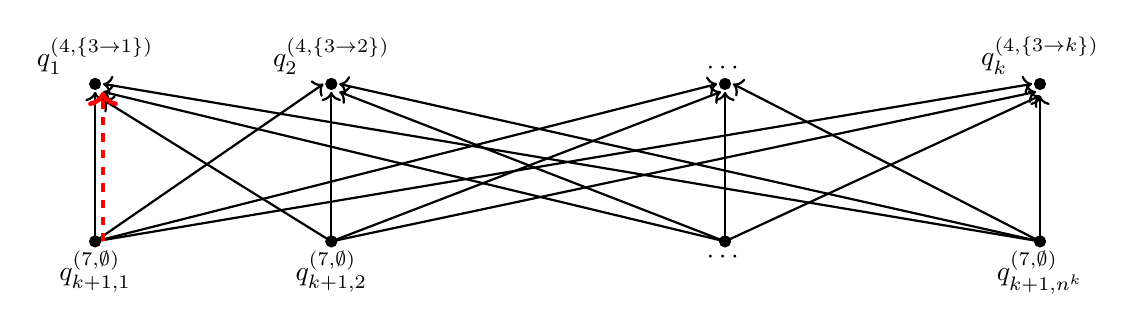
\begin{tikzpicture}
%%% The nodes represents the k query in the first round
\filldraw[black] (0, 2) circle (2pt) node [anchor=south]{$q_1^{(4, \{3 \to 1\} )}$};
\filldraw[black] (3, 2) circle (2pt) node [anchor=south]{$q_2^{(4, \{3 \to 2\} )}$};
% \filldraw[black] (6, 2) circle (2pt) node [anchor=south]{$q^4_3$};
\filldraw[black] (8, 2) circle (2pt) node [anchor=south]{$\cdots$};
\filldraw[black] (12, 2) circle (2pt) node [anchor=south]{$q_k^{(4, \{3 \to k\} )}$};
%%%%%% The nodes represents the n^k queries in the second round
\filldraw[black] (0, 0) circle (2pt) node [anchor=north]{$q_{k+1,1}^{(7, \emptyset)}$};
\filldraw[black] (3, 0) circle (2pt) node [anchor=north]{$q_{k+1,2}^{(7, \emptyset)}$};
% \filldraw[black] (6, 0) circle (2pt) node [anchor=north]{$q^{3, 7}_{k+1}$};
\filldraw[black] (8, 0) circle (2pt) node [anchor=north]{$\cdots$};
\filldraw[black] (12, 0) circle (2pt) node [anchor=north]{$q_{k+1,n^k}^{(7, \emptyset)}$};
%%%%%% The edges represents their dependency relations GROUP 1
\draw[ thick,->] (0, 0)  -- (0, 1.9) ;
\draw[ thick,->] (0, 0)  -- (2.9, 2) ;
% \draw[very thick,->] (0, 0)  -- (6, 2) ;
\draw[ thick,->] (0, 0)  -- (7.9, 2) ;
\draw[ thick,->] (0, 0)  -- (11.9, 2) ;
%%%%%% The edges represents their dependency relations GROUP 2
\draw[ thick,->] (3, 0)  -- (0.1, 1.8) ;
\draw[ thick,->] (3, 0)  -- (3, 1.9) ;
% \draw[very thick,->] (0, 0)  -- (6, 2) ;
\draw[ thick,->] (3, 0)  -- (7.95, 1.9) ;
\draw[ thick,->] (3, 0)  -- (11.95, 1.9) ;
%%%%%% The edges represents their dependency relations GROUP 3
\draw[ thick,->] (8, 0)  -- (0.1, 1.9) ;
\draw[ thick,->] (8, 0)  -- (3.1, 1.9) ;
% \draw[very thick,->] (0, 0)  -- (6, 2) ;
\draw[ thick,->] (8, 0)  -- (8, 1.9) ;
\draw[ thick,->] (8, 0)  -- (12, 1.85) ;
%%%%%% The edges represents their dependency relations GROUP 4
\draw[ thick,->] (12, 0)  -- (0.1, 2) ;
\draw[ thick,->] (12, 0)  -- (3.1, 2) ;
% \draw[very thick,->] (0, 0)  -- (6, 2) ;
\draw[ thick,->] (12, 0)  -- (8.1, 2) ;
\draw[ thick,->] (12, 0)  -- (12, 1.85) ;
%%%% The longest path representing the adaptivity
\draw[ultra thick, red, ->, dashed] (0.1, 0) -- (0.1, 1.9);
\end{tikzpicture}
\end{center}
\end{example}
%
%
\begin{example}[Multi-Round Algorithm]
\[
MR^H \triangleq
\begin{array}{l}
    %  \left[j \leftarrow 0 \right]^1 ; \\
    \left[I \leftarrow [] \right]^1; \\
    \eloop ~ [k]^{2} ~  \\ 
    \ ~ \edo ~ \\ \Big(
    \left[p \leftarrow c \right]^3 ; \\
    \left[a \leftarrow q(p, I) \right]^4; \\
    \left[I \leftarrow \eupdt( {I}, (a, p))  \right]^5
    \Big) 
\end{array}
%
~~~~ \Rightarrow ~~~
%
MR^L \triangleq
\begin{array}{l}
    %  \left[j \leftarrow 0 \right]^1 ; \\
    \left[I \leftarrow [] \right]^1; \\
    \eloop ~ [k]^{2}  \\ 
    \ ~ \edo ~ \\ \Big(
    \left[p \leftarrow c \right]^3 ; \\
    \left[
    \eswitch \Big( I, a
    \left(\begin{array}{l}
        [ ] \to q_{j,1},\\
        \cdots\\
    \clabel{1, 2, 3, \cdots, n} \to q_{j,n!}
    \end{array}\right)
    \Big)
    \right]^4;\\
    \left[I \leftarrow \eupdt( {I}, (a, p))  \right]^5
    \Big) 
\end{array}
%
% \begin{array}{l}
%     \left[I \leftarrow [] \right]^2; \\
%     \ewhile \Big( 
%     \left[j \leq k \right]^3 , \\
%     \left[p \leftarrow 0 \right]^4 ; \\
%     \left[
%     \eswitch \Big( I, x
%     \left(\begin{array}{l}
%         [ ] \to q_{j,1},\\
%         \cdots\\
%     \clabel{1, 2, 3, \cdots, n} \to q_{j,n!}
%     \end{array}\right)
%     \Big)
%     \right]^5\\
%     \clabel{I \leftarrow \eupdt(I, (a, p))}^6;\\
%     \clabel{j \leftarrow j + 1 }^7
%     \Big) ;
% \end{array}
\]
%
%
% Let $k = 4$, given a specific database $D$, we have $\config{\emptyset, MR^L, [],\emptyset} \rightarrow \config{m, \eskip, t, w } $ and the trace as:
% %
% $$t = \left[(q^{4, \{2 \to 1\}}_{1, 1}, v_1), 
% (q^{4, \{2 \to 2\}}_{2, 3}, v_2),
% (q^{4, \{2 \to 3\}}_{3, 2}, v_3)
% (q^{4, \{2 \to 4\}}_{4, 3}, v_4)
% \right]$$
% \\
Adapt($MR^L$) = 2 when $k=2$

\[
MR^{ssa} \triangleq
\begin{array}{l}
    %  \left[j \leftarrow 0 \right]^1 ; \\
    \left[I_1 \leftarrow [] \right]^1; \\
    \eloop ~ [k]^{2} , 0, [I_3,I_1,I_2] \\ 
    \ ~ \edo ~ \\ \Big(
    \left[p_1 \leftarrow c \right]^3 ; \\
    \left[
    \eswitch \Big( I_3, a_1
    \left(\begin{array}{l}
        [ ] \to q_{j,1},\\
        \cdots\\
    \clabel{1, 2, 3, \cdots, n} \to q_{j,n!}
    \end{array}\right)
    \Big)
    \right]^4;\\
    \left[I_2 \leftarrow \eupdt( {I_3}, (a_1, p_1))  \right]^5
    \Big) 
\end{array}
\]
Using \THESYSTEM, we first generate a global list $G$ from an empty list $[]$ and empty whlemap $\emptyset$.
 \[[]; \emptyset; MR^{ssa} \to G; w  \land w = \emptyset\].
 \[G_{k=2} = \left[
  {I_1}^{(1,\emptyset)} , {I_3}^{(2,[2:1])} , {p_1}^{(3,[2:1])} , {a_1}^{(4,[2:1])} ,{I_2}^{(5,[2:1])} ,  {I_3}^{(2,[2:2])} , {p_1}^{(3,[2:2])} , {a_1}^{(4,[2:2])} ,{I_2}^{(5,[2:2])} , {I_3}^{(2,\emptyset)}   \right] \]
  We denote $I_1^{1}$ short for ${I_1}^{(1,\emptyset)}$ and ${I_3}^{(2,1)}$ short for ${I_3}^{(2,[2:1])}$, where the label $(2, 1)$ represents at line number $2$ and in the $1$ st iteration. 
\[
M =  \left[ \begin{matrix}
  I_1^{1} & I_3^{(2,1)} & p_1^{(3,1)} & a_1^{(4,1)} &I_2^{(5,1)}  & I_3^{(2,2)} & p_1^{(3,2)} & a_1^{(4,2)} & I_2^{(5,2)} & I_3^{2}\\
  0 & 0 & 0 & 0 & 0 & 0 & 0 &0 &0&0  \\
 1 & 0 & 0 & 0 & 0 & 0 & 0&0&0&0\\
 0 & 0 & 0 & 0 & 0 & 0& 0& 0 &0&0\\
 0 & 1 & 0 & 0 & 0 & 0 & 0& 0&0&0\\
 0 & 1 & 1 & 1 & 0 & 0 & 0 & 0&0 &0\\
 1 & 0 & 0 & 0 & 1 & 0 & 0& 0&0&0\\
 0 & 0 & 0 & 0 & 0 & 0 & 0& 0&0&0\\
 0 & 0 & 0 & 0 & 0 & 1 & 0& 0&0&0\\
 0 & 0 & 0 & 0 & 0 & 1 & 1 & 1 &0 &0\\
1 & 0 & 0 & 0 & 0 & 0 & 0 & 0 &1&0 \\
 \end{matrix} \right] 
~ , V = \left [ \begin{matrix}
I_1^{1} &  0 \\
I_3^{(2,1)} &  0 \\
p_1^{(3,1)} & 0 \\
a_1^{(4,1)} &  1 \\
I_2^{(5,1)} & 0 \\
I_3^{(2,2)} & 1 \\
p_1^{(3,2)} &  0 \\
a_1^{(4,2)} & 1 \\
I_2^{(5,2)} & 0 \\
I_3^{2} & 0 \\
\end{matrix} \right ]
\]

\begin{center}
%
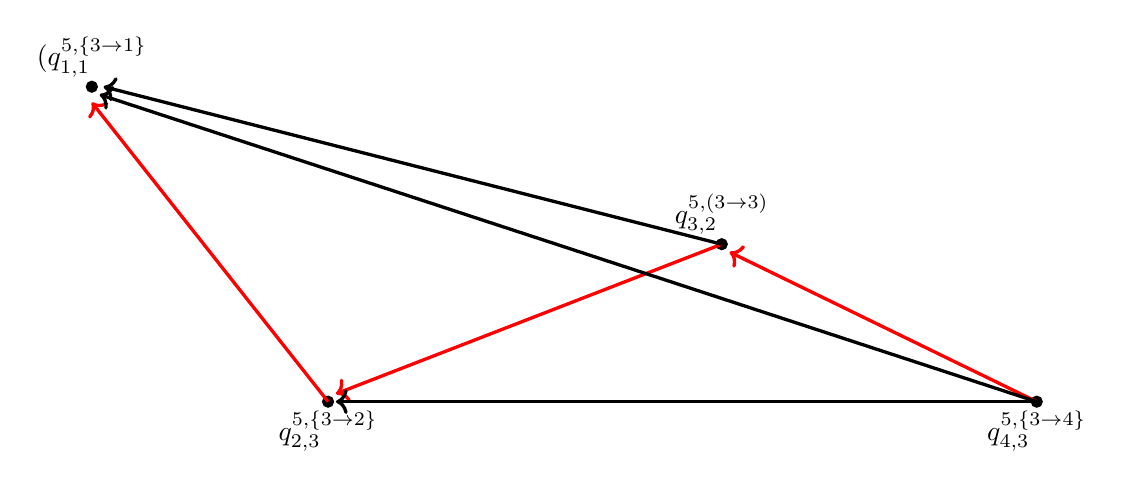
\begin{tikzpicture}
%%% The nodes represents the k query in the first round
\filldraw[black] (0, 4) circle (2pt) node [anchor=south]{$(q^{5, \{3 \to 1\}}_{1, 1}$};
% \filldraw[black] (8, 4) circle (2pt) node [anchor=south]{$\cdots$};
% \filldraw[black] (12, 4) circle (2pt) node [anchor=south]{$q^{1, (5, k)}_k$};
%%%%%% The nodes represents the n^k queries in the second round
% \filldraw[black] (0, 0) circle (2pt) node [anchor=north]{$q^{n!, (5, 1)}_1$};
\filldraw[black] (3, 0) circle (2pt) node [anchor=north]{$q^{5, \{3 \to 2\}}_{2, 3}$};
% \filldraw[black] (6, 0) circle (2pt) node [anchor=north]{$q^{3, 7}_{k+1}$};
% \filldraw[black] (8, 0) circle (2pt) node [anchor=north]{$\cdots$};
\filldraw[black] (12, 0) circle (2pt) node [anchor=north]{$q^{5, \{3 \to 4\}}_{4, 3}$};
%%% The nodes represents the k query in the first round
% \filldraw[black] (0, 2) circle (2pt) node [anchor=south]{$q^{\cdots, (5, 1)}_1$};
% \filldraw[black] (3, 2) circle (2pt) node [anchor=south]{$q^{\cdots, (5, 2)}_2$};
% \filldraw[black] (6, 2) circle (2pt) node [anchor=south]{$q^4_3$};
\filldraw[black] (8, 2) circle (2pt) node [anchor=south]{$q^{5, (3 \to 3)}_{3, 2}$};
% \filldraw[black] (12, 2) circle (2pt) node [anchor=south]{$q^{\cdots, (5, k)}_k$};
%%%%%% The edges represents their dependency relations GROUP 1
% \draw[very thick,->] (3, 2)  -- (0.1, 2) ;
% \draw[very thick,->] (3, 0)  -- (0.1, 1.9) ;
% \draw[very thick,->] (3, 4)  -- (0.1, 2.1) ;
% %
% \draw[very thick,->] (3, 2)  -- (0.1, 0.1) ;
% \draw[very thick,->] (3, 0)  -- (0.1, 0) ;
% \draw[very thick,->] (3, 4)  -- (0, 0.2) ;
% %
% \draw[very thick,->] (3, 2)  -- (0.1, 3.9) ;
\draw[very thick,->, red] (3, 0)  -- (0, 3.8) ;
% \draw[very thick,->] (3, 4)  -- (0, 4) ;
% \draw[very thick,->] (0, 0)  -- (6, 2) ;
%%%%%% The edges represents their dependency relations GROUP 2
% \draw[very thick,->] (0, 0)  -- (6, 2) ;
% \draw[very thick,->] (8, 2)  -- (3.1, 2) ;
% \draw[very thick,->] (8, 0)  -- (3.1, 1.9) ;
% \draw[very thick,->] (8, 4)  -- (3.1, 2.1) ;
%
\draw[very thick,->, red] (8, 2)  -- (3.1, 0.1) ;
\draw[very thick,->] (8, 2)  -- (0.15, 4) ;
% \draw[very thick,->] (8, 0)  -- (3.1, 0) ;
% \draw[very thick,->] (8, 4)  -- (3, 0.2) ;
% %
% \draw[very thick,->] (8, 2)  -- (3.1, 3.9) ;
% \draw[very thick,->] (8, 0)  -- (3, 3.8) ;
% \draw[very thick,->] (8, 4)  -- (3.1, 4) ;
%%%%%% The edges represents their dependency relations GROUP 4
% \draw[very thick,->] (0, 0)  -- (6, 2) ;
% \draw[very thick,->] (12, 2)  -- (8.1, 2) ;
\draw[very thick,->, red] (12, 0)  -- (8.1, 1.9) ;
\draw[very thick,->] (12, 0)  -- (3.1, 0) ;
\draw[very thick,->] (12, 0)  -- (0.1, 3.9) ;
% \draw[very thick,->] (12, 4)  -- (8.1, 2.1) ;
% %
% \draw[very thick,->] (12, 2)  -- (8.1, 0.1) ;
% \draw[very thick,->] (12, 0)  -- (8.1, 0) ;
% \draw[very thick,->] (12, 4)  -- (8, 0.2) ;
% %
% \draw[very thick,->] (12, 2)  -- (8.1, 3.9) ;
% \draw[very thick,->] (12, 0)  -- (8, 3.8) ;
% \draw[very thick,->] (12, 4)  -- (8.1, 4) ;
%
% \draw[very thick,->] (12, 2)  -- (8.1, 3.9) ;

%%%% The longest path representing the adaptivity
% \draw[ultra thick, red, ->, dashed] (3, 4.1)  -- (0.1, 4.1);
% \draw[ultra thick, red, ->, dashed] (8, 4.1)  -- (3.1, 4.1);
% \draw[ultra thick, red, ->, dashed] (12, 4.1)  -- (8.1, 4.1);
\end{tikzpicture}
\end{center}
%
%
$\forall k. \forall D$, we have $A(TR^L) = (k - 1)$ given all possible execution traces.
\begin{center}
%
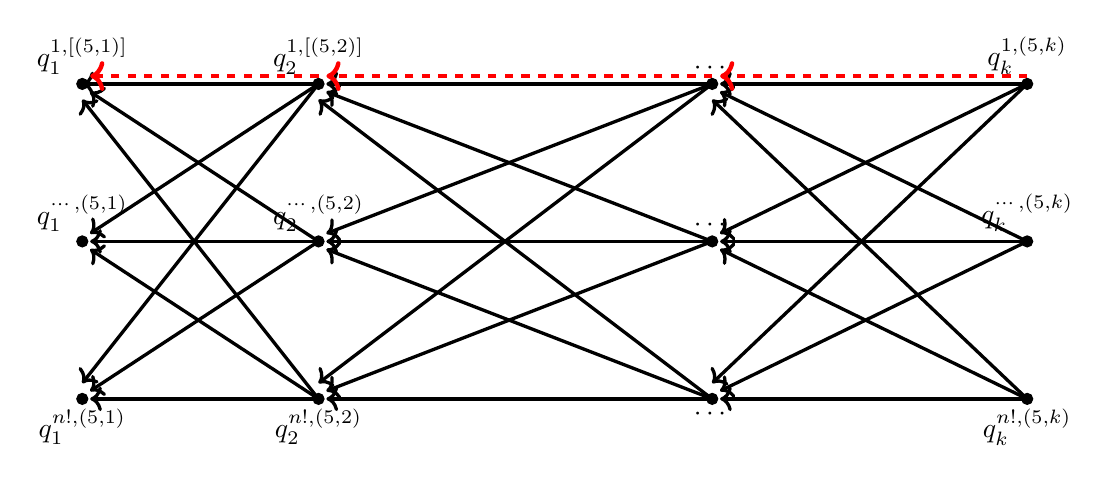
\begin{tikzpicture}
%%% The nodes represents the k query in the first round
\filldraw[black] (0, 4) circle (2pt) node [anchor=south]{$q^{1, [(5, 1)]}_1$};
\filldraw[black] (3, 4) circle (2pt) node [anchor=south]{$q^{1, [(5, 2)]}_2$};
% \filldraw[black] (6, 2) circle (2pt) node [anchor=south]{$q^4_3$};
\filldraw[black] (8, 4) circle (2pt) node [anchor=south]{$\cdots$};
\filldraw[black] (12, 4) circle (2pt) node [anchor=south]{$q^{1, (5, k)}_k$};
%%%%%% The nodes represents the n^k queries in the second round
\filldraw[black] (0, 0) circle (2pt) node [anchor=north]{$q^{n!, (5, 1)}_1$};
\filldraw[black] (3, 0) circle (2pt) node [anchor=north]{$q^{n!, (5, 2)}_2$};
% \filldraw[black] (6, 0) circle (2pt) node [anchor=north]{$q^{3, 7}_{k+1}$};
\filldraw[black] (8, 0) circle (2pt) node [anchor=north]{$\cdots$};
\filldraw[black] (12, 0) circle (2pt) node [anchor=north]{$q^{n!, (5, k)}_k$};
%%% The nodes represents the k query in the first round
\filldraw[black] (0, 2) circle (2pt) node [anchor=south]{$q^{\cdots, (5, 1)}_1$};
\filldraw[black] (3, 2) circle (2pt) node [anchor=south]{$q^{\cdots, (5, 2)}_2$};
% \filldraw[black] (6, 2) circle (2pt) node [anchor=south]{$q^4_3$};
\filldraw[black] (8, 2) circle (2pt) node [anchor=south]{$\cdots$};
\filldraw[black] (12, 2) circle (2pt) node [anchor=south]{$q^{\cdots, (5, k)}_k$};
%%%%%% The edges represents their dependency relations GROUP 1
\draw[very thick,->] (3, 2)  -- (0.1, 2) ;
\draw[very thick,->] (3, 0)  -- (0.1, 1.9) ;
\draw[very thick,->] (3, 4)  -- (0.1, 2.1) ;
%
\draw[very thick,->] (3, 2)  -- (0.1, 0.1) ;
\draw[very thick,->] (3, 0)  -- (0.1, 0) ;
\draw[very thick,->] (3, 4)  -- (0, 0.2) ;
%
\draw[very thick,->] (3, 2)  -- (0.1, 3.9) ;
\draw[very thick,->] (3, 0)  -- (0, 3.8) ;
\draw[very thick,->] (3, 4)  -- (0, 4) ;
% \draw[very thick,->] (0, 0)  -- (6, 2) ;
%%%%%% The edges represents their dependency relations GROUP 2
% \draw[very thick,->] (0, 0)  -- (6, 2) ;
\draw[very thick,->] (8, 2)  -- (3.1, 2) ;
\draw[very thick,->] (8, 0)  -- (3.1, 1.9) ;
\draw[very thick,->] (8, 4)  -- (3.1, 2.1) ;
%
\draw[very thick,->] (8, 2)  -- (3.1, 0.1) ;
\draw[very thick,->] (8, 0)  -- (3.1, 0) ;
\draw[very thick,->] (8, 4)  -- (3, 0.2) ;
%
\draw[very thick,->] (8, 2)  -- (3.1, 3.9) ;
\draw[very thick,->] (8, 0)  -- (3, 3.8) ;
\draw[very thick,->] (8, 4)  -- (3.1, 4) ;
%%%%%% The edges represents their dependency relations GROUP 4
% \draw[very thick,->] (0, 0)  -- (6, 2) ;
\draw[very thick,->] (12, 2)  -- (8.1, 2) ;
\draw[very thick,->] (12, 0)  -- (8.1, 1.9) ;
\draw[very thick,->] (12, 4)  -- (8.1, 2.1) ;
%
\draw[very thick,->] (12, 2)  -- (8.1, 0.1) ;
\draw[very thick,->] (12, 0)  -- (8.1, 0) ;
\draw[very thick,->] (12, 4)  -- (8, 0.2) ;
%
\draw[very thick,->] (12, 2)  -- (8.1, 3.9) ;
\draw[very thick,->] (12, 0)  -- (8, 3.8) ;
\draw[very thick,->] (12, 4)  -- (8.1, 4) ;
%
%%%% The longest path representing the adaptivity
\draw[ultra thick, red, ->, dashed] (3, 4.1)  -- (0.1, 4.1);
\draw[ultra thick, red, ->, dashed] (8, 4.1)  -- (3.1, 4.1);
\draw[ultra thick, red, ->, dashed] (12, 4.1)  -- (8.1, 4.1);
\end{tikzpicture}
\end{center}
\end{example}
%
%
% \begin{thm}
% [Observable Equivalent]
% Given a program $P$ in high level language, the corresponding low level language $P^l$ rewrote from $P$ via the rewriting rules is observably equivalent to $P$.
% \end{thm}
% %
% %
% \subsection{Adaptivity of the High Level Language}
% \begin{defn}
% [Adaptivity]
% Given a program $P$ in high level language, let $P^L$ be the set of all possible program in low level language observable equivalent to $P$, the adaptivity of $P$ is defined as:
% \\
% \[A(P) \triangleq \min\limits_{P^* \in P^L}A^*(P^*) \]
% %
% \end{defn}
% %
% %
% \subsection{Soundness of \THESYSTEM ~ in High Level Language}
% %
% \begin{thm}
% [Soundness]
% Given a program $P$ in high level language, let $P^l$ be the corresponding program in low level rewrote from $P$ via the rewriting rules, 
% then given $\Gamma$, $c_1$ and $c_2$ s.t. $\Gamma \subseteq FreeVar(P^l)$, 
% $ \Gamma \vdash^{c_1, c_2}_{M,V} P^l $, then we have:
% \\
% \[Adaptivity(P) \leq Adapt(M,V) \]
% \end{thm}
% %
% %
% %
% %
% \clearpage
% \section{Towards Probability}
% %
% \subsection{Syntax and Semantics}
% %
% \paragraph{Syntax.}
% \[
% \begin{array}{llll}
%  \mbox{Arithmatic Operators} & *_a & ::= & + ~|~ - ~|~ \times 
% %
% ~|~ \div \\  
%   \mbox{Boolean Operators} & *_b & ::= & \lor \sep \land \\
%   \mbox{Relational Operators} & *_r & ::= & < ~|~ \leq ~|~ = \\  
%  \mbox{Label} & l & & \\ 
%  \mbox{loop maps} & w & \in & \mbox{Label} \times \mathbb{N} \triangleq w +l \sep w \setminus l \sep w \oplus_\rho w \\
% \mbox{AExpr} & \aexpr & ::= & 
% ckk991``	%
% 	n ~|~ x ~|~ \aexpr *_a \aexpr ~|~ {[] ~|~ [\aexpr_0, \dots, \aexpr_i] \sep \aexpr \times \aexpr } \\
%     %
% \mbox{BExpr} & \bexpr & ::= & 
% 	%
% 	\etrue ~|~ \efalse  ~|~ \neg \bexpr
% 	 ~|~ \bexpr *_b \bexpr
% 	%
% 	~|~ \aexpr *_r \aexpr \\
% \mbox{Deterministic Expr} & \expr_d & ::=	& \aexpr \sep \bexpr \\
% \mbox{Randomized AExpr} & \aexpr_r & ::= & 
% 	%
% 	 x_r \sep n \sep  \aexpr_r *_a \aexpr_r \\
%     %
% \mbox{Randomized BExpr} & \bexpr_r & ::= & 
% 	%
% \neg \bexpr_r
% 	 ~|~ \bexpr_r *_b \bexpr_r
% 	%
% 	~|~ \aexpr_r *_r \aexpr_r \\
% \mbox{Randomized Expr} & \expr_r & ::=	& \expr_d \sep \aexpr_r \sep \bexpr_r \\
% \mbox{Command} & \command & ::= &   [\assign x {\expr_d}]^{l} \sep [\assign {x_r} {\expr_r}]^{l} \sep  [\assign x q]^{l} \sep  [\assign {x_r} \uniform ]^{l} \sep   [\assign {x_r} \bernoulli]^{l} 
%  %
% \\
% 	%
% & & & ~|~  \command ; \command  ~|~ \eif_D ([\bexpr]^{l}, \command_1, \command_2) \sep  \eif_R ([\bexpr_r]^{l}, \command_1, \command_2) 
%  ~|~ [\eskip]^{l} \\
% & & & { \sep [\eswitch( \expr, x, (v_i \to  q_i))]^{l}} \sep {\eloop ~ [\valr_N]^{l} ~ (f) ~ \edo ~ \command }
% 	\\
% 	%
% % \mbox{Binary Operation} & \bop & ::= & + ~|~ - ~|~ \times 
% % %
% \mbox{Memory} & m & ::= & [] ~|~ m[x^{l} \to v] \\
% %
% \mbox{Trace} & t & ::= & [] ~|~ [(q, v)^{(l, w) }] ~|~ t ++ t 
% ~|~ t \oplus_{\rho} t
% \end{array}
% \]
% %
% \[
% \begin{array}{ccl}
% w \setminus l     & = &\left \{  
%     \begin{array}{lr} w  & l \not\in Keys(w)   \\
%       w_l & Otherwise \\
%      \end{array} \right.\\
% w + l & = &
%  \left \{  
%     \begin{array}{lr}
%     w[l \to 0] & l \not \in Keys(w) \\   
%     w_l [l \to w(l)+1] & Otherwise
%           \end{array} \right.\\
% \end{array}
% \]
% %
% \paragraph{Semantics}
% We have a countable set $\textsf{RV}$ of random variables($x_r \in \textsf{RV}$), a countable set $\textsf{Val}$ of values. For any subset  $\textsf{S} \subseteq \textsf{RV}$, we denote $\textsf{RanM[S]} \triangleq \textsf{S} \to \textsf{Val} $. We let $\textsf{DV}$ as a countable set of deterministic variables ($x$) and the deterministic memory $\textsf{DetM} \triangleq \textsf{DV} \to \textsf{Val}$. 
% Distribution over A as $D(A)$. The \emph{distribution unit} unit : $A \to D(A)$. The \emph{distribution bind} bind : $ D(A) \to (A \to D(B)) \to D(B)$. $\lrr{C}{} : (\textsf{DetM} \times D(\textsf{RandM}) \times \textsf{Trace} \times \textsf{loop maps} \times \textsf{DB} ) \to (\textsf{DetM} \times D(\textsf{RandM}) \times \textsf{Trace} \times \textsf{loop maps} \times \textsf{DB} ) $

% \[\config{(\sigma, \mu_1 , t_1, w_1, D)} \oplus_{\rho} \config{(\sigma, \mu_2 , t_2, w_2, D)} 
% \triangleq \config{\sigma, \mu_1\oplus_{\rho} \mu_2 , t_1\oplus_{\rho} t_2, w_1 \oplus_{\rho} w_2, D}\]
% %
% \[(t_1 \oplus_{\rho} t_2)  ++ t_3 \triangleq 
% (t_1 ++ t_3) \oplus_{\rho} (t_2 ++ t_3) \]
% %
% \[t_3 ++ (t_1 \oplus_{\rho} t_2) \triangleq 
% (t_3 ++ t_1) \oplus_{\rho} (t_3 ++ t_2) \]
% %
% \[ (w_1 \oplus_{\rho} w_2) + l \triangleq 
% (w_1 + l) \oplus_{\rho} (w_2 + l) \]
% %
% \[ (w_1 \oplus_{\rho} w_2) \setminus l \triangleq 
% (w_1 \setminus l) \oplus_{\rho} (w_2 \setminus l) \]
% \begin{figure}[H]%
%     \centering
%     \[
%     \begin{array}{rll}
%         \lrr{ [\eskip]^{l} }{} (\sigma, \mu , t, w, D) & \triangleq & (\sigma, \mu , t, w , D)  \\
%         \lrr{ [\assign x {\expr_d}]^{l} }{} (\sigma, \mu , t, w, D)  & \triangleq & (\sigma[x \to \lrr{\expr_d}{}(\sigma)], \mu , t, w, D) \\
%         \lrr{ [\assign {x_r} {\expr_r}]^{l}}{} (\sigma, \mu , t, w, D)  & \triangleq & (\sigma, bind(\mu , m \to unit(m[x_r \to \lrr{\expr_r}{}(\sigma, m)]) ) , t, w , D ) \\
%         \lrr{ [\assign x q]^{l} }{} (\sigma, \mu , t, w, D)  & \triangleq & (\sigma[x \to v ], \mu , t ++ [(q, v)]^{(l, w)}, w , D) \qquad : v = q(D)\\
%         \lrr{ [\assign {x_r} \uniform ]^{l} }{} (\sigma, \mu , t, w, D)  & \triangleq & (\sigma,  bind(\mu , m \to bind(\uniform , u \to m[x_r \to u] ) )  , t, w, D) \\
%         \lrr{ [\assign {x_r} \bernoulli ]^{l} }{} (\sigma, \mu , t, w , D)  & \triangleq & (\sigma , bind(\mu , m \to bind(\bernoulli , u \to m[x_r \to u] ) ) , t, w,D) \\
%             \lrr{ \command ; \command' }{} (\sigma, \mu , t, w , D)  & \triangleq & \lrr{\command'}{} ( \lrr{\command}{} \sigma , \mu, t, w) \\
%          \lrr{ \eif_D ([\bexpr]^{l}, \command_1, \command_2)  }{} (\sigma, \mu , t, w , D)  & \triangleq & \left \{  \begin{array}{l} 
%          \lrr{\command_1}{} (\sigma , \mu, t, w, D) \qquad : \lrr{\bexpr}{}(\sigma) = \etrue \\ 
%          \lrr{\command_1}{} (\sigma , \mu, t, w,D) \qquad : \lrr{\bexpr}{}(\sigma) = \efalse \end{array} \right . \\    
%           \lrr{ \eif_R ([\bexpr_r]^{l}, \command_1, \command_2)  }{} (\sigma, \mu , t, w , D)  & \triangleq & \left \{
%           \begin{array}{l}
%           \lrr{\command_1}{} (\sigma , \mu | \lrr{\bexpr_r}{} \sigma = \etrue  , t, w, D) \oplus_\rho  \lrr{\command_2}{} (\rho , \mu | \lrr{\bexpr_r}{} \sigma = \efalse  , t, w,D)  \\ 
%           \lrr{\command_1}{} (\sigma , \mu | \lrr{\bexpr_r}{} \sigma = \etrue  , t, w, D) \qquad \rho = 1 \\
%           \lrr{\command_2}{} (\sigma , \mu | \lrr{\bexpr_r}{} \sigma = \efalse  , t, w,D) \qquad \rho = 0 \\
%             \end{array} \right . \\
%              & & \textsf{where} \quad \rho = \mu (\lrr{\bexpr_r}{} \sigma = \etrue ) \\
%         %   \lrr{ \ewhile([\bexpr]^{l}, \command) }{} (\sigma, \mu , t, w , D)  & \triangleq & \lrr{\eunfold{[\bexpr]^{l}}{ \ewhile([\bexpr]^{l}, \command) }   }{} (\sigma, \mu , t, w , D) \\
%         %   \lrr{ \eunfold{[\bexpr]^{l}}{\command}  }{} (\sigma, \mu , t, w , D)  & \triangleq & \left \{  \begin{array}{l} \lrr{\command}{} (\sigma , \mu, t, w + l, D) \qquad : \lrr{\bexpr}{}(\sigma) = \etrue \\ \lrr{\eskip}{} (\sigma , \mu, t, w-l, D) \qquad : \lrr{\bexpr}{}(\sigma) = \efalse \end{array} \right . \\  
%           \lrr{ {[\eswitch( \expr, x, (v_i \to  q_i))]^{l}} }{} (\sigma, \mu , t, w , D)  & \triangleq & 
%           \lrr{ [\assign x q_1]^{l} }{} ( \sigma, \mu , t, w, D ) 
%           \qquad : v_1 = \lrr{\expr}{}{(\sigma)} \\ 
%           \lrr{ {\eloop ~ [\expr_N]^{l} ~ (f) ~ \edo ~ \command } }{} (\sigma, \mu , t, w , D)  & \triangleq & \left \{  \begin{array}{l} \lrr{f;\command; \eloop ~ [\expr_N-1]^{l} ~ (f) ~ \edo ~ \command }{} (\sigma , \mu, t, w + l, D) \qquad : \lrr{\expr_N}{}(\sigma) >0 \\ \lrr{\eskip}{} (\sigma , \mu, t, w-l, D) \qquad : \lrr{\expr_N}{}(\sigma) = 0 \end{array} \right . \\  
%     \end{array}
%     \]
%     \caption{Semantics of programs}
%     \label{fig:semantics_prob}
% \end{figure}
% %
% %
% % \[
% % \begin{array}{l}
% %      \left[j \leftarrow 0 \right]^1 ; \\
% %     \left[I \leftarrow [] \right]^2; \\
% %     \ewhile \Big( 
% %     \left[j \leq k \right]^3 , \\
% %     \left[p \leftarrow 0 \right]^4 ; \\
% %     \left[
% %     \eswitch \Big( I, x
% %     \left(\begin{array}{l}
% %         [ ] \to q_{j,1},\\
% %         \cdots\\
% %     \clabel{1, 2, 3, \cdots, n} \to q_{j,n!}
% %     \end{array}\right)
% %     \Big)
% %     \right]^5\\
% %     \clabel{I \leftarrow \eupdt(I, (x, p))}^6;\\
% %     \clabel{j \leftarrow j + 1 }^7
% %     \Big) ;
% % \end{array}
% % %
% % ~~~~ \Rightarrow ~~~
% % %
% % SSA \triangleq
% % \begin{array}{l}
% %      \left[j \leftarrow 0 \right]^1 ; \\
% %     \left[I_1 \leftarrow [] \right]^2; \\
% %     \ewhile \Big( 
% %     \left[j \leq k \right]^3 , \phi: {I_2} = f({I_1}, {I_3}) \\
% %     \left[p \leftarrow 0 \right]^4 ; \\
% %     \left[
% %     \eswitch \Big( {I_2}, x
% %     \left(\begin{array}{l}
% %         [ ] \to q_{j,1},\\
% %         \cdots\\
% %     \clabel{1, 2, 3, \cdots, n} \to q_{j,n!}
% %     \end{array}\right)
% %     \Big)
% %     \right]^5\\
% %     \clabel{{I_3} \leftarrow \eupdt({I_2}, (x, p))}^6;\\
% %     \clabel{j \leftarrow j + 1 }^7
% %     \Big) ;
% % \end{array}
% % \]
% % %
% %
% \subsection{Extending Adaptivity onto Probabilistic Program}
% %
% \begin{defn}
% Dependency Forest.
% \\
% Given a program $P$, a database $D$, 
% dependency forest $F(P, D) \triangleq \{ G_1, G_2, \cdots, G_m \}$,
% $G_k = (V_k, E_k)$ is defined as: 
% \\
% $V_k =\{q^{l,w} |\forall m, w. \config{\emptyset, P, D,[], \emptyset } \rightarrow \config{m, \eskip, D, T, \emptyset} \land q^{l,w} \in \pi_k (T)  \}$;
% \\
% $E_k = \left\{(q_i^{l,w},q_j^{l',w'}) 
% ~ \left \vert ~ \neg \mathsf{IND}(q_i^{l,w},q_j^{l',w'}, P)
% \land \mathsf{To}(q_j^{l',w'}, q_i^{l,w}) \right.\right\}$,
% \\
% where $\pi_k (T) = t_k$ s.t. $T = t_1 \oplus_{\rho_1} t_2 \oplus_{\rho_2}
% \cdots \oplus_{m - 1} t_m $ and there is no $\oplus$ in $t_i$.
% \end{defn}

% \begin{defn}
% Dependency Graph.
% \\
% Given a program $P$, a database $D$, 
% dependency graph $G(P, D) \triangleq (V, E)$ is defined as: 
% \\
% $V =\bigcup \{V_k | G_k \in F(P, D)  \}$;
% \\
% $E_k = \left\{(q_i,q_j) 
% ~ \left \vert ~ (q_i,q_j) \in E_k , G_k \in F(P, D) \right.\right\}$,
% \end{defn}
% %
% %
% \begin{defn}
% Adaptivity.
% \\
% Given a program $P$ and for all the database $D$ in a set of $DBS$ of databases, the total dependency graph G is the combination of all the dependent graphs over every single database $G(P, D) = (V, E)$, the adaptivity of the program is defined as $A(P)$, s.t.:
% for every pair $(i,j)$ let $p_{(i,j)}$ be the longest path starting from $q_i^{l, w}$ to $q_j^{l',w'}$,
% %
% $$A(P) = \max\limits_{q_i^{l,w},q_j^{l',w'} \in V }\{l_i ~|~ l_i = |p_(i,j)| \}$$
% \end{defn}
% %
% %
\section{Analysis of Generalization Error}

\begin{example}[Two Round Algorithm]
\[
TR^H(k) \triangleq
{
\begin{array}{l}
    % \left[j \leftarrow 0 \right]^1 ; \\
    \clabel{a_1 \leftarrow [] }^1; \\
    \eloop ~ [k]^{2} ~ (a_2 \leftarrow f(1, a_1, a_3)) \\
    ~ \edo ~ \\
    \Big(
     \clabel{x_1 \leftarrow q() }^3 ; \\
    \clabel{a_3 \leftarrow x_1 :: a_2 }^4     \Big);\\
    \clabel{l \leftarrow q_{k + 1}(a_3)}^{5}\\
\end{array}
}
\]
\end{example}
%
\begin{example}[Multi-Round Algorithm]
\[
MR^H \triangleq
\begin{array}{l}
    %  \left[j \leftarrow 0 \right]^1 ; \\
    \left[I_2 \leftarrow [] \right]^1; \\
    \eloop ~ [k]^{2} ~ (I_2 \leftarrow f(2, I_1, I_3)) \\ 
    \ ~ \edo ~ \\ \Big(
    \left[p_1 \leftarrow c \right]^3 ; \\
    \left[a_1 \leftarrow \delta(q(p, I_2)) \right]^4; \\
    \left[I_3 \leftarrow \eupdt( {I_2}, (a_1, p))  \right]^5
    \Big) 
\end{array}
\]
\end{example}
%
%
By applying different mechanisms $\delta()$ over the queries $q(\cdot)$, we have different error bounds.
\\
\textbf{Gaussian Mechanism:} $N(0, \sigma)$ \cite{dwork2015preserving}:
\\
Adaptivity $r = 2$: 
$ \sigma = O \left(\frac{\sqrt{r \log(k)}}{\sqrt{n}} \right)$ (also known as expected error);
\\
Adaptivity unknown:
$ \sigma = O\left(\frac{\sqrt[4]{k}}{\sqrt{n}} \right)$;
\\
{Mean Squared Error Bound:} 
$ \frac{1}{2n} \min\limits_{\lambda \in [0, 1]}
\left( \frac{2\rho k n - \ln(1 - \lambda)}{\lambda} 
\right)
+ 2 \mathbb{E}_{Z_i \sim N(0, \frac{1}{2n^2 \rho})}
\left[ \max\limits_{i \in [k]} (Z_i^2) \right]$
%
\\
{Confidence Bounds:} minimize $\tau$ where
$\tau \geq \sqrt{\frac{2}{n \beta}
\min\limits_{\lambda \in [0, 1]}
\left( \frac{2\rho k n - \ln(1 - \lambda)}{\lambda} 
\right)
}$
and 
$\tau \geq \frac{2}{n} \sqrt{\frac{\ln(4n /\beta}{\rho'}}$ with confidence level $1 - \beta$ .
\\
\textbf{$(\epsilon, \delta)-DP$ mechanism}:
\\
Confidence Bounds:
$\tau \geq \sqrt{\frac{48}{n} \ln(4/\beta) }$ with $\epsilon \leq \frac{\tau}{4}$ and $\delta = 
\exp \left(\frac{-4 \ln (8/\beta)}{\tau} \right)$
\\
\textbf{Sample Splitting}: 
\\
Expected Error: $O \left(\frac{\sqrt{k \log(k)}}{\sqrt{n}} \right)$
\\
\textbf{Thresholdout}: $B, \sigma, T, h$ 
\\
Confidence bounds:  
$\tau = \max\limits\left\{ 
\sqrt{\frac{2\zeta }{h \beta}},
2\sigma \ln(\frac{\beta}{2}),
\sqrt{\frac{1}{\beta}} \cdot \left(\sqrt{T^2 + 56\sigma^2} + \sqrt{\frac{\zeta}{4h} } \right)
\right\}
$,
for $\zeta = \min\limits_{\lambda \in [0, 1)}
\left( \frac{2B \ (\sigma^2 h) - \ln(1 - \lambda)}{\lambda} \right)$


% \begin{mathpar}
% \inferrule
% {M = \mathsf{L}(i) * ( \mathsf{R}(\expr,i) + \Gamma )
% }
% {\Gamma \vdash_{M, V_{\emptyset}}^{(i, i+1)} \assign {x}{\expr} 
% }
% ~\textbf{asgn}
% \and
% \inferrule
% {M = \mathsf{L}(i) * ( \Gamma)
% \\
% V= \mathsf{L}(i)
% }
% { \Gamma \vdash^{(i, i+1)}_{M, V} \assign{x}{q} : 
% }~\textbf{query}
% %
% \and 
% %
% \inferrule
% {
% \Gamma + \mathsf{R}(\bexpr) \vdash^{(i_1, i_2)}_{M, V} c_1 
% : \Phi \land \bexpr \Rightarrow \Psi
% \and 
% \Gamma + \mathsf{R}(\bexpr) \vdash^{(i_2, i_3)}_{M, V} c_2 
% : \Phi \land \neg \bexpr \Rightarrow \Psi
% }
% {
% \Gamma \vdash^{(i_1, i_3)}_{M, V} 
% \eif ~ \bexpr \ethen c_1 \eelse c_2 : \Phi \Rightarrow \Psi
% }~\textbf{if}
% %
% %
% %
% \and 
% %
% \inferrule
% {
% \Gamma \vdash^{(i_1, i_2)}_{M_1, V_1} c_1 : \Phi \Rightarrow \Phi_1
% \and 
% \Gamma \vdash^{(i_2, i_3)}_{M_2, V_2} c_2 : \Phi_1 \Rightarrow \Psi 
% }
% {
% \Gamma \vdash^{(i_1, i_3)}_{M_1 ; M_2, V_1 \uplus V_2}
% c_1 ; c_2 : \Phi \Rightarrow \Psi
% }
% ~\textbf{seq}
% \and 
% \inferrule
% {
% \forall 0 \leq z < N. 
% {\Gamma \vdash^{(i,i+a )}_{M_1, V_1} c_1 : \Phi \land e_n = \lceil{z+1}\rceil \Rightarrow \Psi }
% \and
% {\Gamma \vdash^{(i+a,i+b )}_{M, V} c_2 : \Psi \Rightarrow \Phi \land e_N = \lceil{z}\rceil }
% \and
% { e_N = \lceil {N} \rceil }
% }
% {\Gamma \vdash^{(i, i+ N*b)}_{M_{i,b}^N(c_1), V_{i, b}^N} 
% \eloop ~ \expr_N ~ (c_1) ~ \edo ~ c_2 : \Phi \land \expr_N = \lceil { N} \rceil \Rightarrow \Phi \land \expr_N = \lceil{0}\rceil
% }~\textbf{loop}
% % \and 
% % \inferrule
% % {
% % \Gamma \vdash^{(i,i+a )}_{M, V} c 
% % }
% % {\Gamma \vdash^{(i, i+ N*a)}_{M_{i,a}^N(f), V_{i, a}^N} 
% % \ewhile([\bexpr]^l,   c) : \phi \Rightarrow \psi
% % }~\textbf{while}
% %
% \and
% %
% \inferrule
% { \Gamma + \mathsf{R}(\expr) \vdash^{(i_1+j-1, i_1+j)}_{M_j, V_j} \assign{ x_j}{q_j} : \Phi \Rightarrow \Psi
% \\
% j \in \{1, \dots, N\}     }
% {\Gamma \vdash^{(i_1, i_1+N)}_{ \sum_{j=0}^{N} M_j, \sum_{j=0}^{N} V_j} \eswitch(\expr, x,(v_j \rightarrow q_j ) : \Phi \Rightarrow \Psi }
% ~\textbf{switch}
% %
% \and
% %
% \inferrule
% { 
% \vDash 
% \Phi \Rightarrow \Phi'  
% \and
% \Gamma \vdash^{(i_1, i_2)}_{(M',V')} c : \Phi' \Rightarrow \Psi'
% \and
% \vDash \Psi' \Rightarrow \Psi
% \and 
% \Phi \vDash M' \leq M
% \and 
% \Phi \vDash V' \leq V
% }
% {\Gamma \vdash^{(i_1, i_2)}_{(M,V)} c 
% : \Phi \Rightarrow \Psi
% }
% ~\textbf{conseq}
% \end{mathpar}

\clearpage

\section{new \THESYSTEM with loop }
\subsection{Analysis Rules/Algorithms of \THESYSTEM}

There are two steps for our algorithm to get the estimation of the adaptivity of a program $\ssa{c}$ in the ssa form. 
\begin{enumerate}
    \item Estimate the variables that are new generated (via assignment) and store these variables in a global list $G$. We have the algorithm of the form : $\ag{ G;w; \ssa{c}}{G';w'} $.
    \item We start to track the dependence between variables in a matrix $M$, whose size is $|G| \times |G|$, and track whether arbitrary variable is assigned with a query result in a vector $V$ with size $|G|$. The algorithm to fill in the matrix is of the form: $\ad{\Gamma ; \ssa{c} ; i_1}{M;V;{i_2}}$. $\Gamma$ is a vector records the variables the current program $\ssa{c}$ depends on, the index $i_1$ is a pointer which refers to the position of the first new-generated variable in $\ssa{c}$ in the global list $G$, and $i_2$ points to the first new variable that is not in $\ssa{c}$ (if exists). 
\end{enumerate}

% We have the judgment of the form $\vdash^{i_1, i_2}_{M,V} ~ c  $.  Our grade is a combination of a matrix $M$, used to track the dependency of variables appeared in the statement $c$, and a vector $V$ indicating the variables associated with results from queries $q$. The size of the matrix $M$ is $L \times L$, and vector $V$ of size $L$, where $L$ is the total size of variables needed in the program $c$, which is fixed per program. We assume the program is in the style of Static Single Assignment.To be more specific, we give a quick example: $x \leftarrow e_1; x \leftarrow e_2 $ will be rewritten as $ x_1 \leftarrow e_1; x_2 \leftarrow e_2$. And the if condition $ \eif ~ e_b \ethen x \leftarrow e_1 \eelse x \leftarrow e_2  $ will look like $ \eif ~ e_b \ethen x_1 \leftarrow e_1 \eelse x_2 \leftarrow e_2  $. As we have seen, SSA requires unique variables, and these newly generated variables will be recorded in the matrix $M$.  Also, the variable at different iteration is treated as different variable in the matrix $M$ and vector $V$.

% The superscript $i_1,i_2$  specify the range of "living" or "active" variables in the matrix and vector. $i_1$ is the starting line (and column) in the matrix where the new generated variables in program $c$ starts to show up. Likewise, $i_2$ states the ending position of active range by $c$.
%  Worth to mention, $i_1,i_2$ can be used to track the exact location of newly generated variables. For example, the assignment statement $x \leftarrow e$ or $x \leftarrow q $ with $c_2 =c_1+1$, tells us the variable $x$ is at the $c_1$th line(column) of the matrix. As we can notice, the loop increases the variables needed in the matrix by $N \times a$ where $N$ is the number of rounds of the loop and $a$ is the size of the variables generated in the loop body. We will have a global map, which maps the variable name to the position in the vector. We call it $GM: VAR \to \mathbb{N}$.

We give an example of $M$ and $V$ of the program $c$.   
$$
c= \begin{array}{c}
\ssa{\assign {x_1} {q}} ;        \\
\ssa{\assign {x_2} {x_1+1}} ;\\
\ssa{\assign {x_3} {x_2+2} }
\end{array}~~~~~~~~~~~~
M =  \left[ \begin{matrix}
 & (x_1) & (x_2) & (x_3) \\
(x_1) & 0 & 0 & 0 \\
(x_2) & 1 & 0 & 0 \\
(x_3) & 1 & 1 & 0 \\
\end{matrix} \right] ~ , V = \left [ \begin{matrix}
(x_1) &  1 \\
(x_2) & 0 \\
(x_3) & 0 \\
\end{matrix} \right ]
$$
Still use the program $c$ as the example, the global list $G$ is now : $ [ x_1 , x_2 , x_3] $. 
The function $\mathsf{Left}$ and $\mathsf{Right}$ is used to generate the corresponding vector of the left side and right side of an assignment. Take $\assign {x_2} {x_1+1} $ as an example, the result is shown as follows.
\[
\sf{L}(1) = \left[ \begin{matrix}
 0  & ~~~(x_1) \\
 1 & ~~~(x_2) \\
 0 & ~~~(x_3) \\
\end{matrix}   \right ] ~~~~~~~~~~~~~~
\sf{R} (x_1+1, 1) = \left[ \begin{matrix} 
   1 & 0 & 0 \\
   (x_1) & (x_2) & (x_3) \\
\end{matrix}  \right]
\]
Now let us think about the loop.
\[\ssa{c_3} \triangleq
\begin{array}{l}
     \left[\ssa{ x_1 \leftarrow q_1}  \right]^1 ; \\
    \eloop ~ [2]^{2} , 0,\\
  \ssa{[x_3 , x_1 , x_2]} 
     ~ \edo
    \\
    ~ \Big( 
    \left[\ssa{ y_1 \leftarrow q_2} \right]^3; \\
    \left[\ssa{x_2 \leftarrow y_1  + x_3 } \right]^5
    \Big) ; \\
     \left[ \assign{z_1}{x_3 + 2}  \right]^{6}
\end{array}
~~~~~~~~~~~~
M =  \left[ \begin{matrix}
 & (x_1) & (x_3^{1}) & (y_1^{1}) & (x_3^{1})  & (x_3^{2}) & (y_1^{2}) & (x_2^{2}) & (x_3^{f}) &  (z_1) \\
(x_1) & 0 & 0 & 0 & 0 & 0 & 0 & 0 &0 &0 \\
(x_3^{1}) & 1 & 0 & 0 & 0 & 0 & 0 & 0&0&0\\
(y_1^{1}) & 0 & 0 & 0 & 0 & 0 & 0& 0& 0 &0\\
(x_2^{1}) & 0 & 1 & 1 & 0 & 0 & 0 & 0& 0&0\\
(x_3^{2}) & 0 & 0 & 0 & 1 & 0 & 0 & 0 & 0&0 \\
(y_1^{2}) & 0 & 0 & 0 & 0 & 0 & 0 & 0& 0&0\\
(x_2^{2}) & 0 & 0 & 0 & 0 & 1 & 1 & 0& 0&0\\
(x_3^{f}) & 1 & 0 & 0 & 0 & 0 & 0 & 1& 0&0\\
(z_1) & 0 & 0 & 0 & 0 & 0 & 0 & 0 & 1 &0 \\
\end{matrix} \right] ~ , V = \left [ \begin{matrix}
(x_1) &  1 \\
(x_3^{1}) & 0 \\
(y_1^{1}) & 1 \\
(x_2^{1}) &  0 \\
(x_3^{2}) & 0 \\
(y_1^{2}) & 1 \\
(x_2^{2}) &  0 \\
(x_3^{f}) &  0 \\
(z_1) &  0 \\
\end{matrix} \right ]
\]

\[\ssa{c_3'} \triangleq
\begin{array}{l}
     \left[\ssa{ x_1 \leftarrow q_1}  \right]^1 ; \\
    \eloop ~ [0]^{2} , 0,\\
  \ssa{[x_3 , x_1 , x_2]} 
     ~ \edo
    \\
    ~ \Big( 
    \left[\ssa{ y_1 \leftarrow q_2} \right]^3; \\
    \left[\ssa{x_2 \leftarrow y_1  + x_3 } \right]^5
    \Big) ; \\
    \left[ \assign{z_1}{x_3 + 2}  \right]^{6}
\end{array}
~~~~~~~~~~~~
M =  \left[ \begin{matrix}
 & (x_1) & (x_3^{f}) & (z_1)  \\
(x_1) & 0 & 0 & 0 \\
(x_3^{f}) & 1 & 0 & 0 \\
(z_1^{2}) & 0 & 1 & 0 \\
\end{matrix} \right] ~ , V = \left [ \begin{matrix}
(x_1) &  1 \\
(x_3^{f}) & 0 \\
(z_1) &  0 \\
\end{matrix} \right ]
\]
We can now look at the if statement.
\[ c_4 \triangleq
\begin{array}{l}
   \left[ x \leftarrow q_1 \right]^1; \\
   \left[y \leftarrow q_2\right]^2 ; \\
    \eif \;( x + y == 5 )^3\; \\
    \mathsf{then} \;\left[ x \leftarrow q_3 \right]^4 \; \\
    \mathsf{else} (\;\left[ x \leftarrow q_4 \right]^5 ; \\
    y \leftarrow 2 ) ;\\
   \left[ z \leftarrow x +y \right]^6; \\
\end{array}
\hspace{20pt} \hookrightarrow \hspace{20pt}
%
 \ssa{c_4} \triangleq
\begin{array}{l}
   \left[ \ssa{ x_1 \leftarrow q_1} \right]^1; \\
   \left[\ssa{ y_1 \leftarrow q_2} \right]^2 ; \\
    \eif \;( \ssa{ x_1 + y_1 == 5} )^3, [ x_4,x_2,x_3 ],[] ,[y_3,y_1,y_2 ]\; \\
    \mathsf{then} \;\left[ \ssa{ x_2 \leftarrow q_3}\right]^4 \; \\
    \mathsf{else} (\;\left[ \ssa{x_3 \leftarrow q_4} \right]^5 ; \\
     \ssa{y_2 \leftarrow 2} ) \\
   \left[ \ssa{ z_1 \leftarrow x_4 +y_3 }\right]^6; \\
\end{array}
\]
\[
M_{c4} =  \left[ \begin{matrix}
 & (x_1) & (y_1) & (x_2) & (x_3)  & (y_2) & (x_4) & (y_3) & (z_1)  \\
(x_1) & 0 & 0 & 0 & 0 & 0 & 0 & 0 &0  \\
(y_1) & 0 & 0 & 0 & 0 & 0 & 0 & 0&0\\
(x_2) & 0 & 0 & 0 & 0 & 0 & 0& 0& 0 \\
(x_3) & 0 & 0 & 0 & 0 & 0 & 0 & 0& 0\\
(y_2) & 0 & 0 & 0 & 0 & 0 & 0 & 0 & 0 \\
(x_4) & 0 & 0 & 1 & 1 & 0 & 0 & 0 &0\\
(y_3) & 0 & 1 & 0 & 0 & 1 & 0 & 0 &0\\
(z_1) & 0 & 0 & 0 & 0 & 0 & 1 & 1 & 0  \\
\end{matrix} \right] ~ , V_{c4} = \left [ \begin{matrix}
(x_1) &  1 \\
(y_1) & 1 \\
(x_2) & 1 \\
(x_3) &  1 \\
(y_2) & 0 \\
(x_4) & 0 \\
(y_3) &  0 \\
(z_1) &  0 \\
\end{matrix} \right ]
\]
% We consider to have the superscript to denote the iteration number (or map if we have nested loop), as shown in the above matrix and vector. The global map $G$ is generated by analysing the program. We can estimate the variables needed in the loop by using the loop number $N$ and the loop body. In this example, the global map for $c_3$ : $ \{ x_1 \to 1, x_2^{1} \to 2, y_1^{1} \to 3 , x_3^{1} \to 4 , x_2^{2} \to 5 , y_1^{2} \to 6 , x_3^{2} \to 7  \} $.  
% By default, $G(x_2)$ gives the location for the first appearance of the variable $x_2$. We can also allow $G(x_2 , 2)$ to get the location of the second iteration $x_2^{2}$. We also allow $G(x, i, i+n)$ to return a set of locations where $x$ appears in the vector in the certain range $[i, i+n]$, which helps to locate variables in the loop.




% Also, to be able to track the relation between variables in varied iterations in the loop. we define a dependent map $\mathsf{DM}$ based on command $c$ to provide the dependency relation(syntactically) between variables. $\mathsf{VAR}(\expr)$ gives the set of variables appears in the expression $\expr$.
% \[
% \begin{array}{lll}
% \mathsf{DM} (c_1; c_2) & \triangleq &  \mathsf{DM} (c_1) \uplus \mathsf{DM} (c_2)  \\
% \mathsf{DM} (x_1 \leftarrow \expr ) & \triangleq & \{  x_1 \to \mathsf{VARS}(\expr)  \}
% \end{array}
% \]

\subsection{The algorithm to estimate the matrix and vector}
We first generate a list of variables $G$ that will be assigned with values (via the command $\assign{x}{e}$ or $\assign{x}{q}$). 

 \begin{mathpar}
\inferrule
{
}
{ \ag{G ;w; \ssa{[\assign {x}{\expr}]^{l}}}{G ++ [\ssa{x}^{(l,w)}];w}
% G ;w; \ssa{[\assign {x}{\expr}]^{l}} \to G ++ [x^{(l,w)}];w 
}
~\textbf{ag-asgn}
\and
\inferrule
{
}
{ \ag{G ;w;  [ \assign{\ssa{x}}{q(\ssa{\expr})}]^{l}}{  G ++ [\ssa{x}^{(l,w)}] ; w} 
}~\textbf{ag-query}
%
\and 
%
\inferrule
{
\ag{G; w; \ssa{c_1}}{  G_1;w_1}
\and 
 \ag{G_1;w ; \ssa{c_2}}{  G_2; w_2}
 \\
 {G_3 = G_2 ++ \ssa{[\bar{x}^{(l,w)}]++ \ssa{[\bar{y}^{(l,w)}]}++ \ssa{[\bar{z}^{(l,w)}]} }}
}
{
\ag{G; w;
[\eif(\ssa{\bexpr},[ \bar{\ssa{x}}, \bar{\ssa{x_1}}, \bar{\ssa{x_2}}] ,[ \bar{\ssa{y}}, \bar{\ssa{y_1}}, \bar{\ssa{y_2}}],[ \bar{\ssa{z}}, \bar{\ssa{z_1}}, \bar{\ssa{z_2}}], \ssa{ c_1, c_2)}]^{l} }{ G_3 ;w}
}~\textbf{ag-if}
%
%
%
\and 
%
\inferrule
{
\ag{G; w; \ssa{c_1}}{ G_1; w_1}
\and 
\ag{G_1;w_1; \ssa{c_2}}{ G_2; w_2}
}
{
\ag{G; w;
\ssa{(c_1 ; c_2)}}{  G_2 ; w_2}
}
~\textbf{ag-seq}
\and 
\inferrule
{
{G_0 = G \quad w_0 =w }
\and
\forall 0 \leq z < N. 
{ \ag{ G_z ++ \ssa{[\bar{x}^{(l, {w_z}+l)}]} ; (w_z+l); \ssa{c}}{ G_{z+1} ; w_{z+1}}  }
\\
{G_f = G_N ++ \ssa{[\bar{x}^{(l, w_N \setminus l)}]} }
\and
{ \ssa{\aexpr} =  {N}  }
}
{\ag{G; w; [\eloop ~ \ssa{\aexpr}, n, [\bar{\ssa{x}}, \bar{\ssa{x_1}}, \bar{\ssa{x_2}}] ~ \edo ~ \ssa{c}]^{l} }{ G_f; w_N\setminus l }
}~\textbf{ag-loop}
\end{mathpar}


%
%
% \paragraph{Analysis Rules.}
% \[\begin{array}{ll}
%     \mathcal{A}( \assign x \expr )( \Gamma , i )  & =  ( \mathsf{L}(x) * ( \mathsf{R}(\expr) + \Gamma ), V, i+1 )\\
%     \mathcal{A}( \assign x q)( \Gamma ,  i )  & = ( \mathsf{L}(x) * ( \mathsf{R}(\emptyset) + \Gamma) , \mathsf{L}(x) , i+1 )\\
%     \mathcal{A}( \eif ~ e_b \ethen c_1 \eelse c_2 )( \Gamma , i ) & =   \elet \; (M_1, v_1, i_1) =  \mathcal{A}(C_1)(\Gamma +\mathsf{R}(e_b) , i)
%     \ein \; \\
%     &  \elet \;  (M_2, v_2, i_2)= \mathcal{A}(C_2) (\Gamma +\mathsf{R}(e_b) ,i_1) \ein \; \\
%     & (  M_1 \uplus M_2, V_1 \uplus V_2   , i_2 )
%     \\
%     \mathcal{A}( c_1 ; c_2 )( \Gamma ,  i )  & =  \elet \;     (M_1, v_1, i_1) = 
%     \mathcal{A}(c_1) (\Gamma  +\mathsf{R}(e_b) , i)
%     \ein \; \\
%     &  \elet \;  (M_2, v_2, i_2) =                      \mathcal{A}(c_2)(\Gamma +\mathsf{R}(e_b) ,
%       i_1) \ein \; \\ 
%       & (  M_1 \cdot M_2, V_1 \uplus V_2   , i_2 )    \\
%      \mathcal{A}( \eloop ~ \expr_N ~ (c_1) ~ \edo ~ c_2  )( \Gamma ,  i )  & =  \elet \;     (M_1, v_1, i+a) = 
%     \mathcal{A}(c_1;c_2 ) (\Gamma , i)
%     \ein \; \\
%     & ( M_{i,a}^N(c_1), V_{i, a}^N , i + N*a ) \\
%  \mathcal{A}( \eswitch(\expr, x,(v_j \rightarrow q_j )  )( \Gamma ,  i+j )  & =  \elet \;     (M_j, v_j, i+j) = 
%     \mathcal{A}(x_j \leftarrow q_j ) (\Gamma + \mathsf{R}(e), i+j-1)     
%   \ein \\
%   & ( \sum_{j=0}^{N} M_j, \sum_{j=0}^{N} V_j, i + N ) \quad j \in \{1, \dots, N\}  \\
%     \end{array}
% \]
%
%
\paragraph{Analysis Logic Rules.}
%
%
$\Gamma$ is a matrix of one row and $N$ columns, $N = |G|=|V|$.\\ 

$\mathsf{L(i)}$ generates a matrix of one column, $N$ rows, where the $i-th$ row is $1$, all the other rows are $0$.\\

$\mathsf{R(e, i)}$ generates a matrix of one row and $N$ columns, where the locations of variables in $e$ is marked as $1$. To handle loop, for instance, the variable $y$ appears many times in $G$, the argument $i$ helps to find the location of the current living variable $y$ in the expression $e$, which is the latest $y$ with the largest location $i_y< i$ in our global variable list $G$.\\ 


{$ \forall 0 \leq z < |\bar{x}|. \bar{x}(z) = x_z, \bar{x_1}(z) = x_{1z}, \bar{x_2}(z) = x_{2z} $ } \\

$ \Gamma \vdash_{M,v_{\emptyset}}^{i, i+ |\ssa{\bar{x}}|} \ssa{[ \bar{x},\bar{x_1},\bar{x_2}   ]} \triangleq { \forall 0 \leq z < |\bar{x}|.  \Gamma \vdash_{M_{x_z}, V_{\emptyset}}^{i+z, i+z+1 } x_z \leftarrow x_{1z} + x_{2z} }$ where $M = \sum_{z\in [|\bar{x}|] }M_{x_z} $\\

\framebox{$ {\Gamma} \vdash^{i_1, i_2}_{M,V} ~ c $}
%
% \begin{mathpar}
% \inferrule
% {M = \mathsf{L}(i) * ( \mathsf{R}(\expr,i) + \Gamma )
% }
% {\Gamma \vdash_{M, V_{\emptyset}}^{(i, i+1)} [\assign {\ssa{x}}{\ssa{\expr}} ]^{l}
% }
% ~\textbf{asgn}
% \and
% \inferrule
% {M = \mathsf{L}(i) * ( \Gamma)
% \\
% V= \mathsf{L}(i)
% }
% { \Gamma \vdash^{(i, i+1)}_{M, V} [ \assign{\ssa{x}}{q} ]^{l} 
% }~\textbf{query}
% %
% \and 
% %
% \inferrule
% {
% \Gamma + \mathsf{R}(\bexpr, i_1) \vdash^{(i_1, i_2)}_{M_1, V_1} \ssa{c_1} 
% % : \Phi \land \bexpr \Rightarrow \Psi
% \and 
% \Gamma + \mathsf{R}(\bexpr, i_1) \vdash^{(i_2, i_3)}_{M_2, V_2} \ssa{c_2} 
% % : \Phi \land \neg \bexpr \Rightarrow \Psi
% \\
% { \forall 0 \leq j < |\bar{x}|. \bar{x}(j) = x_j, \bar{x_1}(j) = x_{1j}, \bar{x_2}(j) = x_{2j}  }
% \\
% { \forall 0 \leq j < |\bar{x}|.  \Gamma \vdash_{M_{x_j}, V_{\emptyset}}^{i_3+j, i_3+j+1 } x_j \leftarrow x_{1j} + x_{2j} }
% \and
% { \forall 0 \leq j < |\bar{y}|.  \Gamma \vdash_{M_{y_j}, V_{\emptyset}}^{i_3+|\bar{x}|+j, i_3+|\bar{x}|+j+1 } y_j \leftarrow y_{1j} + y_{2j} }
% \\
% { \forall 0 \leq j < |\bar{z}|.  \Gamma \vdash_{M_{z_j}, V_{\emptyset}}^{i_3+|\bar{x}|+|\bar{y}|+j, i_3+|\bar{x}|+|\bar{y}|+j+1 } z_j \leftarrow z_{1j} + z_{2j} }
% \and
% {M = (M_1+M_2)+ \sum_{j\in [|\bar{x}|] }M_{x_j} + \sum_{j\in [|\bar{y}|] }M_{y_j} + \sum_{j\in [|\bar{z}|] }M_{z_j} }
% }
% {
% \Gamma \vdash^{(i_1, i_3+|\bar{x}|+|\bar{y}|+|\bar{z}|)}_{M, V_1 \uplus V_2 } 
% [\eif(\sbexpr,[ \bar{\ssa{x}}, \bar{\ssa{x_1}}, \bar{\ssa{x_2}}] ,[ \bar{\ssa{y}}, \bar{\ssa{y_1}}, \bar{\ssa{y_2}}] , [ \bar{\ssa{z}}, \bar{\ssa{z_1}}, \bar{\ssa{z_2}}] , \ssa{ c_1, c_2)}]^{l}
% }~\textbf{if}
% %
% %
% %
% \and 
% %
% \inferrule
% {
% \Gamma \vdash^{(i_1, i_2)}_{M_1, V_1} \ssa{c_1} 
% % : \Phi \Rightarrow \Phi_1
% \and 
% \Gamma \vdash^{(i_2, i_3)}_{M_2, V_2} \ssa{c_2} 
% % : \Phi_1 \Rightarrow \Psi 
% }
% {
% \Gamma \vdash^{(i_1, i_3)}_{M_1 \green{;} M_2, V_1 \uplus V_2}
% \ssa{c_1 ; c_2} 
% % : \Phi \Rightarrow \Psi
% }
% ~\textbf{seq}
% \and 
% \inferrule
% {
% B= |\ssa{\bar{x}}| 
% \and
% {\Gamma \vdash^{(i, i+B)}_{M_{10}, V_{10}} [\bar{\ssa{x}}, \bar{\ssa{x_1}}, \bar{\ssa{x_2}}] }
% \and
% {\Gamma \vdash^{(i+B,i+B+A )}_{M_{20}, V_{20}} \ssa{c} 
% }
% \\
% \forall 1 \leq j < N. 
% {\Gamma \vdash^{(i+j*(B+A), i+B+j*(B+A))}_{M_{1j}, V_{1j}}  } [\bar{\ssa{x}}, \bar{\ssa{x_1}}, \bar{\ssa{x_2}}]
% \and
% {\Gamma \vdash^{(i+B+j*(B+A),i+B+A+j*(B+A) )}_{M_{2j}, V_{2j}} \ssa{c} 
% % : \Phi \land e_n = \lceil{z+1}\rceil \Rightarrow \Psi 
% }
% \\
% {\Gamma \vdash^{(i+N*(B+A) ,i+N*(B+A)+B )}_{M, V} [\bar{\ssa{x}}, \bar{\ssa{x_1}}, \bar{\ssa{x_2}}]
% % : \Psi \Rightarrow \Phi \land e_N = \lceil{z}\rceil 
% }
% \and
% { \ssa{a} = \lceil {N} \rceil }
% \and
% {M' = M+ \sum_{0 \leq j <N} M_{1j}+M_{2j}  }
% \and
% {V' = V \uplus \sum_{0 \leq j <N} V_{1j} \uplus V_{2j}  }
% }
% {\Gamma \vdash^{(i, i+N*(B+A)+B   )}_{M', V'} 
% [\eloop ~ \ssa{\aexpr}, 0, [\bar{\ssa{x}}, \bar{\ssa{x_1}}, \bar{\ssa{x_2}}] ~ \edo ~ \ssa{c}]^{l}
% % : \Phi \land \expr_N = \lceil { N} \rceil \Rightarrow \Phi \land \expr_N = \lceil{0}\rceil
% }~\textbf{loop}
% % \and 
% % \inferrule
% % {
% % \Gamma \vdash^{(i,i+a )}_{M, V} c 
% % }
% % {\Gamma \vdash^{(i, i+ N*a)}_{M_{i,a}^N(f), V_{i, a}^N} 
% % \ewhile([\bexpr]^l,   c) : \phi \Rightarrow \psi
% % }~\textbf{while}
% %
% \and
% %
% \inferrule
% { \Gamma + \mathsf{R}(\expr,i) \vdash^{(i, i+1)}_{M, V} \assign{ x}{q_j} 
% % : \Phi \Rightarrow \Psi
% \\
% j \in \{1, \dots, N\}     }
% {\Gamma \vdash^{(i, i+1)}_{ M,V } 
% [\eswitch(\ssa{\expr}, \ssa{x},(v_j \rightarrow q_j ) ]^{l}
% % : \Phi \Rightarrow \Psi 
% }
% ~\textbf{switch}
% % %
% % \and
% % %
% % \inferrule
% % { 
% % \vDash 
% % \Phi \Rightarrow \Phi'  
% % \and
% % \Gamma \vdash^{(i_1, i_2)}_{(M',V')} c : \Phi' \Rightarrow \Psi'
% % \and
% % \vDash \Psi' \Rightarrow \Psi
% % \and 
% % \Phi \vDash M' \leq M
% % \and 
% % \Phi \vDash V' \leq V
% % }
% % {\Gamma \vdash^{(i_1, i_2)}_{(M,V)} c 
% % : \Phi \Rightarrow \Psi
% % }
% % ~\textbf{conseq}
% \end{mathpar}
\begin{mathpar}
\inferrule
{M = \mathsf{L}(i) * ( \mathsf{R}(\ssa{\expr},i) + \Gamma )
}
{
 \ad{\Gamma;[\assign {\ssa{x}}{\ssa{\expr}} ]^{l}; i }{M; V_{\emptyset}; i+1 }
% \Gamma \vdash_{M, V_{\emptyset}}^{(i, i+1)} [\assign {\ssa{x}}{\ssa{\expr}} ]^{l}
}
~\textbf{ad-asgn}
\and
\inferrule
{M = \mathsf{L}(i) * ( \mathsf{R}(\ssa{\expr},i) + \Gamma )
\\
V= \mathsf{L}(i)
}
{ 
\ad{\Gamma;[ \assign{\ssa{x}}{q(\ssa{\expr})} ]^{l} ; i }{M;V;i+1}
%  \vdash^{(i, i+1)}_{M, V} [ \assign{\ssa{x}}{q(\ssa{\expr})} ]^{l} 
}~\textbf{ad-query}
%
\and 
%
\inferrule
{
{\ad{\Gamma + \mathsf{R}(\ssa{\bexpr}, i_1); \ssa{c_1} ; i_1 }{ M_1;V_1;i_2 }}
% \Gamma + \mathsf{R}(\bexpr, i_1) \vdash^{(i_1, i_2)}_{M_1, V_1} \ssa{c_1} 
% : \Phi \land \bexpr \Rightarrow \Psi
\and 
{\ad{\Gamma + \mathsf{R}(\ssa{\bexpr}, i_1);\ssa{c_2} ; i_2 }{ M_2; V_2 ;i_3}}
% \Gamma + \mathsf{R}(\ssa{\bexpr}, i_1) \vdash^{(i_2, i_3)}_{M_2, V_2} \ssa{c_2} 
% : \Phi \land \neg \bexpr \Rightarrow \Psi
\\
% { \forall 0 \leq j < |\bar{x}|. \bar{x}(j) = x_j, \bar{x_1}(j) = x_{1j}, \bar{x_2}(j) = x_{2j}  }
{\ad{\Gamma; [ \bar{\ssa{x}}, \bar{\ssa{x_1}}, \bar{\ssa{x_2}}]; i_3 }{ M_x; V_{\emptyset}; i_3+|\bar{\ssa{x}}| }}
%
\and
%
{\ad{\Gamma; [ \bar{\ssa{y}}, \bar{\ssa{y_1}}, \bar{\ssa{y_2}}]; i_3+|\bar{\ssa{x}}| }{ M_y; V_{\emptyset}; i_3+|\bar{\ssa{x}}|+|\bar{\ssa{y}}| }}
%
\\
%
{\ad{\Gamma; [ \bar{\ssa{z}}, \bar{\ssa{z_1}}, \bar{\ssa{z_2}}]; i_3+|\bar{\ssa{x}}|+ |\bar{\ssa{y}}|}{ M_y; V_{\emptyset}; i_3+|\bar{\ssa{x}}|+|\bar{\ssa{y}}| + |\bar{\ssa{z}}| }}
\\
{M = (M_1+M_2)+ M_x+M_y +M_z }
}
{
\ad{\Gamma ; \eif([\ssa{\bexpr}]^{l},[ \bar{\ssa{x}}, \bar{\ssa{x_1}}, \bar{\ssa{x_2}}] ,[ \bar{\ssa{y}}, \bar{\ssa{y_1}}, \bar{\ssa{y_2}}] , [ \bar{\ssa{z}}, \bar{\ssa{z_1}}, \bar{\ssa{z_2}}] , \ssa{ c_1, c_2)} ; i_1}{ M ;V_1 \uplus V_2  ; i_3+|\bar{x}|+|\bar{y}|+|\bar{z}| }
}~\textbf{ad-if}
%
%
%
\and 
%
\inferrule
{
{\ad{\Gamma; \ssa{c_1} ; i_1 }{ M_1 ; V_1; i_2 }  }
% \Gamma \vdash^{(i_1, i_2)}_{M_1, V_1} \ssa{c_1} 
% : \Phi \Rightarrow \Phi_1
\and 
{\ad{\Gamma;\ssa{c_2}; i_2}{M_2; V_2 ;i_3 }}
% \Gamma \vdash^{(i_2, i_3)}_{M_2, V_2} \ssa{c_2} 
% : \Phi_1 \Rightarrow \Psi 
}
{
\ad{\Gamma ; (\ssa{c_1 ; c_2} ) ; i_1}{(M_1 {;} M_2) ; V_1 \uplus V_2 ; i_3  }
% \Gamma \vdash^{(i_1, i_3)}_{M_1 {;} M_2, V_1 \uplus V_2}
% \ssa{c_1 ; c_2} 
% : \Phi \Rightarrow \Psi
}
~\textbf{ad-seq}
\and 
\inferrule
{
B= |\ssa{\bar{x}}| \and {A = |\ssa{c}|}
% \and
% {\Gamma \vdash^{(i, i+B)}_{M_{10}, V_{10}} [\bar{\ssa{x}}, \bar{\ssa{x_1}}, \bar{\ssa{x_2}}] }
% \and
% {\Gamma \vdash^{(i+B,i+B+A )}_{M_{20}, V_{20}} \ssa{c} 
% }
\\
\forall 0 \leq j < N. 
{\ad{\Gamma;[\bar{\ssa{x}}, \bar{\ssa{x_1}}, \bar{\ssa{x_2}}]; i+ j*(B+A) }{M_{1j};V_{1j}; i+B+j*(B+A) }}
% {\Gamma \vdash^{(i+j*(B+A), i+B+j*(B+A))}_{M_{1j}, V_{1j}}  } [\bar{\ssa{x}}, \bar{\ssa{x_1}}, \bar{\ssa{x_2}}]
\\
{
\ad{\Gamma;\ssa{c} ; i+B+j*(B+A)  }{M_{2j}; V_{2j}; i+B+A+j*(B+A) }
% \Gamma \vdash^{(i+B+j*(B+A),i+B+A+j*(B+A) )}_{M_{2j}, V_{2j}} \ssa{c} 
% : \Phi \land e_n = \lceil{z+1}\rceil \Rightarrow \Psi 
}
\\
{
\ad{\Gamma ; [\bar{\ssa{x}}, \bar{\ssa{x_1}}, \bar{\ssa{x_2}}] ; i+N*(B+A) }{M; V ;i+N*(B+A)+B}
% \Gamma \vdash^{(i+N*(B+A) ,i+N*(B+A)+B )}_{M, V} [\bar{\ssa{x}}, \bar{\ssa{x_1}}, \bar{\ssa{x_2}}]
% : \Psi \Rightarrow \Phi \land e_N = \lceil{z}\rceil 
}
\\
{ \ssa{\aexpr} =  {N}  }
\and
{M' = M+ \sum_{0 \leq j <N}( M_{1j}+M_{2j})  }
\and
{V' = V \uplus \sum_{0 \leq j <N}( V_{1j} \uplus V_{2j})  }
}
{
\ad{\Gamma;\eloop ~ [\ssa{\aexpr}]^{l}, ~0, [\bar{\ssa{x}}, \bar{\ssa{x_1}}, \bar{\ssa{x_2}}] ~ \edo ~ \ssa{c}, i }{ M';V' ;i+N*(B+A)+B }
%  \vdash^{(i,   )}_{M', V'} 
% : \Phi \land \expr_N = \lceil { N} \rceil \Rightarrow \Phi \land \expr_N = \lceil{0}\rceil
}~\textbf{ad-loop}
\end{mathpar}
%
\begin{figure}
   \[
 \begin{array}{lll}
    |[\eswitch(\ssa{\expr}, \ssa{x},(v_j \rightarrow q_j )]^{l} |_{low}  &=& [\eswitch(|\ssa{\expr}|_{low}, |x|_{low},(v_j \rightarrow q_j )]^{l} \\
    | [\eloop ~ \ssa{\aexpr}, n, [\bar{\ssa{x}}, \bar{\ssa{x_1}}, \bar{\ssa{x_2}}] ~ \edo ~ \ssa{c}]^{l}|_{low}  &=& [\eloop ~ |\ssa{\aexpr}|_{low},  ~ \edo ~ |\ssa{c}|_{low}]^{l} \\
      |\ssa{c_1 ; c_2}|_{low}  &=& |\ssa{c_1}|_{low} ; |\ssa{c_2}|_{low} \\
       |[\eif(\sbexpr,[ \bar{\ssa{x}}, \bar{\ssa{x_1}}, \bar{\ssa{x_2}}] ,[ \bar{\ssa{y}}, \bar{\ssa{y_1}}, \bar{\ssa{y_2}}] , [ \bar{\ssa{z}}, \bar{\ssa{z_1}}, \bar{\ssa{z_2}}] , \ssa{ c_1, c_2)}]^{l}|_{low}  &=&
       [\eif(|\sbexpr|_{low}, |\ssa{ c_1}|_{low}, |\ssa{c_2}|_{low})]^{l}\\
       | [\assign {\ssa{x}}{\ssa{\expr}}]^{l}|_{low} & = & [\assign {|\ssa{x}|_{low}}{|\ssa{\expr}|_{low}} ]^{l}  \\
       | [\assign {\ssa{x}}{q} ]^{l} |_{low} & = & [\assign {|\ssa{x}|_{low}}{q}]^{l} \\
       |x_i|_{low} & = & x \\
       |n |_{low} & = & n \\
      | \ssa{\aexpr_1} \oplus_{a} \ssa{\aexpr_2} |_{low} & = &  |\ssa{\aexpr_1}|_{low} \oplus_a |\ssa{\aexpr_2}|_{low} \\
      | \ssa{\bexpr_1} \oplus_{b} \ssa{\bexpr_2} |_{low} & = &  |\ssa{\bexpr_1}|_{low} \oplus_b |\ssa{\bexpr_2}|_{low}
 \end{array}
\]
    \caption{The erasure of SSA}
    \label{fig:ssa_erasure}
\end{figure}


\[
\begin{array}{lll}
M_1 ; M_2 & := & M_2 \cdot M_1 + M_1 + M_2      \\
V_1 \uplus V_2 & := & \left\{
\begin{array}{ll}
1 & (V_1[i] = 1 \lor V_2[i] = 1) \land i = 1, \cdots, N \land |V_1| = |V_2|\\
0 & o.w.
\end{array}\right.\\
%
% M_1 \uplus M_2 & := & \left\{
% \begin{array}{ll}
% 1 & (M_1[i][j] = 1  \lor M_2[i][j] = 1) \land i, j = 1, \cdots, N \land |M_1| = |M_2|\\
% 0 & (M_1[i][j] = 0  \land M_2[i, j] = 0) \land i, j = 1, \cdots, N \land |M_1| = |M_2|\\
% \bot & o.w.
% \end{array}\right.\\
%
% V_{(i, a)}^N
% & := & \left\{
% \begin{array}{ll}
% V[i+ o*a, i + (o + 1) * a-1] = V[i, i + a-1] & 
%  o = 1, \cdots, N - 1 \\
% \bot & o.w.
% \end{array}\right.\\
% %
% M_{(i, a)}^N (c)
% & := & \left\{
% \begin{array}{ll}
% M[i+ o*a, i + (o + 1) * a-1][i + o*a, i + (o + 1) * a-1] & \\
% = M[i, i + a-1][i, i+ a-1] & 
%  o = 1, \cdots, N - 1 \\
% M[i+ o*a,i + (o + 1) * a-1][0, i + o * a-1] = 
% 0 & 
%  o = 1, \cdots, N - 1 \\
% M[0, i + o * a-1][i+ o*a, i + (o + 1) * a-1] & \\
% =  M[0, i + (o - 1) * a-1][i+ (o - 1)*a, i + o * a-1] & 
%  o = 1, \cdots, N - 1 \\
%  \qquad & \qquad  \qquad  \\
% M[l][k] = 
% 1& 
% \begin{array}{l}
% \forall x_l \in  \mathsf{DM}(c). \forall x_k \in  \mathsf{DM}(c)(x_l).\\
%  for \quad o = 0, \cdots, N . \\
% l \in G(x_l,i+ o*a, i+(o+1)*a-1) \land \\
% k \in G(x_k,0, i + (o ) * a-1) \land \\
% \end{array}\\
% \bot & o.w.
% \end{array}\right.\\
%
\end{array}
\]
%
% \begin{center}
% \begin{tabular}{p{15pt}|p{15pt}|p{15pt}||p{15pt}|p{15pt}
% |p{15pt}||p{15pt}|p{15pt}|
% p{15pt}|p{15pt}|p{15pt}|p{15pt}|p{15pt}| } 
%  1 & $\cdots$ & i-1 & i & $\cdots$ & \tiny{i+a-1} & {\tiny i+a } 
% & $\cdots$ & {\tiny{i+2a-1} }
% & $\cdots$ & {\tiny i+N*a-1} & {\tiny i+N*a} & $\cdots$ \\
% \hline
% $\cdots$  & \cellcolor{green} & \cellcolor{green} & \cellcolor{sandstorm} 0 & \cellcolor{sandstorm} 0 & \cellcolor{sandstorm} 0 & \cellcolor{sandstorm} 0 & \cellcolor{sandstorm} 0 & \cellcolor{sandstorm} 0 &  &  &  & \\[10pt]
% \hline
% i-1 & \cellcolor{green} & \cellcolor{green} & \cellcolor{sandstorm} 0 & \cellcolor{sandstorm} 0 & \cellcolor{sandstorm} 0 & \cellcolor{sandstorm} 0 &\cellcolor{sandstorm} 0 & \cellcolor{sandstorm} 0 &  &  &  &  \\ [10pt]
% \hline
% i & \cellcolor{periwinkle} & \cellcolor{periwinkle} & \cellcolor{pink} & \cellcolor{pink} &\cellcolor{pink} & \cellcolor{sandstorm} 0 &
% \cellcolor{sandstorm} 0 &
% \cellcolor{sandstorm} 0 &&&& \\ [10pt]
% \hline
% $\cdots$ & \cellcolor{periwinkle} & \cellcolor{periwinkle}
% &\cellcolor{pink} &\cellcolor{pink}&\cellcolor{pink} &
% \cellcolor{sandstorm} 0 & \cellcolor{sandstorm} 0 &
% \cellcolor{sandstorm} 0 &&&& \\ [10pt]
% \hline
% i+a-1 &\cellcolor{periwinkle} &\cellcolor{periwinkle} & \cellcolor{pink} & \cellcolor{pink} & \cellcolor{pink} 
% & \cellcolor{sandstorm} 0 & \cellcolor{sandstorm} 0 
% & \cellcolor{sandstorm} 0 &&&& \\ [10pt]
% \hline \hline
% {\scriptsize i+a }  & \cellcolor{periwinkle} & \cellcolor{periwinkle} & \cellcolor{trueblue} &\cellcolor{trueblue}
% & \cellcolor{trueblue}& \cellcolor{pink} 
% &\cellcolor{pink} & \cellcolor{pink} & &&& \\ [10pt]
% \hline
% $\cdots$ &\cellcolor{periwinkle} &\cellcolor{periwinkle} & \cellcolor{trueblue}  & \cellcolor{trueblue} c & \cellcolor{trueblue} 
% & \cellcolor{pink} & \cellcolor{pink} &\cellcolor{pink} 
% &&&& \\ [10pt]
% \hline
% {\small i+2a-1 } &\cellcolor{periwinkle} & \cellcolor{periwinkle} & \cellcolor{trueblue} 
% & \cellcolor{trueblue}  & \cellcolor{trueblue}
% & \cellcolor{pink} & \cellcolor{pink} & \cellcolor{pink} 
% &&&& \\ [10pt]
% \hline
% $\cdots$ & &&&&&&&&&&&  \\ [10pt]
% \hline
% {\tiny i+N*a-1 } & &&&&&&&&&&& \\ [10pt]
% \hline
% {\tiny i+N*a} & &&&&&&&&&&&\\ [10pt]
% \hline
% $\cdots$ & &&&&&&&&&&&\\ [10pt]
% \hline
% \end{tabular}
% \end{center}
%
%
%
       
% \begin{defn}
% [Validity of hoare triple]
% If $ c : \psi \Rightarrow \phi$, for any memory $m$ and database $D$ s.t., $\psi(m)$ holds, for any trace $t$, loop maps $w$ so that $ \config{m, c, t,w} \rightarrow^{*} \config{m', \eskip, t', w'}$, then $\phi(m')$ holds, written $\vDash c : \psi \Rightarrow \phi $.  
% \end{defn}




\newpage
\bibliographystyle{plain}
\bibliography{adaptivity.bib}

\end{document}



